\documentclass[twoside]{book}

% Packages required by doxygen
\usepackage{fixltx2e}
\usepackage{calc}
\usepackage{doxygen}
\usepackage[export]{adjustbox} % also loads graphicx
\usepackage{graphicx}
\usepackage[utf8]{inputenc}
\usepackage{makeidx}
\usepackage{multicol}
\usepackage{multirow}
\PassOptionsToPackage{warn}{textcomp}
\usepackage{textcomp}
\usepackage[nointegrals]{wasysym}
\usepackage[table]{xcolor}

% Font selection
\usepackage[T1]{fontenc}
\usepackage[scaled=.90]{helvet}
\usepackage{courier}
\usepackage{amssymb}
\usepackage{sectsty}
\renewcommand{\familydefault}{\sfdefault}
\allsectionsfont{%
  \fontseries{bc}\selectfont%
  \color{darkgray}%
}
\renewcommand{\DoxyLabelFont}{%
  \fontseries{bc}\selectfont%
  \color{darkgray}%
}
\newcommand{\+}{\discretionary{\mbox{\scriptsize$\hookleftarrow$}}{}{}}

% Page & text layout
\usepackage{geometry}
\geometry{%
  a4paper,%
  top=2.5cm,%
  bottom=2.5cm,%
  left=2.5cm,%
  right=2.5cm%
}
\tolerance=750
\hfuzz=15pt
\hbadness=750
\setlength{\emergencystretch}{15pt}
\setlength{\parindent}{0cm}
\setlength{\parskip}{3ex plus 2ex minus 2ex}
\makeatletter
\renewcommand{\paragraph}{%
  \@startsection{paragraph}{4}{0ex}{-1.0ex}{1.0ex}{%
    \normalfont\normalsize\bfseries\SS@parafont%
  }%
}
\renewcommand{\subparagraph}{%
  \@startsection{subparagraph}{5}{0ex}{-1.0ex}{1.0ex}{%
    \normalfont\normalsize\bfseries\SS@subparafont%
  }%
}
\makeatother

% Headers & footers
\usepackage{fancyhdr}
\pagestyle{fancyplain}
\fancyhead[LE]{\fancyplain{}{\bfseries\thepage}}
\fancyhead[CE]{\fancyplain{}{}}
\fancyhead[RE]{\fancyplain{}{\bfseries\leftmark}}
\fancyhead[LO]{\fancyplain{}{\bfseries\rightmark}}
\fancyhead[CO]{\fancyplain{}{}}
\fancyhead[RO]{\fancyplain{}{\bfseries\thepage}}
\fancyfoot[LE]{\fancyplain{}{}}
\fancyfoot[CE]{\fancyplain{}{}}
\fancyfoot[RE]{\fancyplain{}{\bfseries\scriptsize Generated by Doxygen }}
\fancyfoot[LO]{\fancyplain{}{\bfseries\scriptsize Generated by Doxygen }}
\fancyfoot[CO]{\fancyplain{}{}}
\fancyfoot[RO]{\fancyplain{}{}}
\renewcommand{\footrulewidth}{0.4pt}
\renewcommand{\chaptermark}[1]{%
  \markboth{#1}{}%
}
\renewcommand{\sectionmark}[1]{%
  \markright{\thesection\ #1}%
}

% Indices & bibliography
\usepackage{natbib}
\usepackage[titles]{tocloft}
\setcounter{tocdepth}{3}
\setcounter{secnumdepth}{5}
\makeindex

% Hyperlinks (required, but should be loaded last)
\usepackage{ifpdf}
\ifpdf
  \usepackage[pdftex,pagebackref=true]{hyperref}
\else
  \usepackage[ps2pdf,pagebackref=true]{hyperref}
\fi
\hypersetup{%
  colorlinks=true,%
  linkcolor=blue,%
  citecolor=blue,%
  unicode%
}

% Custom commands
\newcommand{\clearemptydoublepage}{%
  \newpage{\pagestyle{empty}\cleardoublepage}%
}

\usepackage{caption}
\captionsetup{labelsep=space,justification=centering,font={bf},singlelinecheck=off,skip=4pt,position=top}

%===== C O N T E N T S =====

\begin{document}

% Titlepage & ToC
\hypersetup{pageanchor=false,
             bookmarksnumbered=true,
             pdfencoding=unicode
            }
\pagenumbering{alph}
\begin{titlepage}
\vspace*{7cm}
\begin{center}%
{\Large py\+P\+L\+A\+N\+ES }\\
\vspace*{1cm}
{\large Generated by Doxygen 1.8.14}\\
\end{center}
\end{titlepage}
\clearemptydoublepage
\pagenumbering{roman}
\tableofcontents
\clearemptydoublepage
\pagenumbering{arabic}
\hypersetup{pageanchor=true}

%--- Begin generated contents ---
\chapter{Hierarchical Index}
\section{Class Hierarchy}
This inheritance list is sorted roughly, but not completely, alphabetically\+:\begin{DoxyCompactList}
\item \contentsline{section}{py\+P\+L\+A\+N\+E\+S.\+classes.\+fem\+\_\+classes.\+Bubble}{\pageref{classpy_p_l_a_n_e_s_1_1classes_1_1fem__classes_1_1_bubble}}{}
\item \contentsline{section}{py\+P\+L\+A\+N\+E\+S.\+classes.\+calculus.\+Calculus}{\pageref{classpy_p_l_a_n_e_s_1_1classes_1_1calculus_1_1_calculus}}{}
\begin{DoxyCompactList}
\item \contentsline{section}{py\+P\+L\+A\+N\+E\+S.\+classes.\+calculus.\+Fem\+Calculus}{\pageref{classpy_p_l_a_n_e_s_1_1classes_1_1calculus_1_1_fem_calculus}}{}
\begin{DoxyCompactList}
\item \contentsline{section}{py\+P\+L\+A\+N\+E\+S.\+classes.\+fem\+\_\+problem.\+Fem\+Problem}{\pageref{classpy_p_l_a_n_e_s_1_1classes_1_1fem__problem_1_1_fem_problem}}{}
\end{DoxyCompactList}
\item \contentsline{section}{py\+P\+L\+A\+N\+E\+S.\+classes.\+calculus.\+Pw\+Calculus}{\pageref{classpy_p_l_a_n_e_s_1_1classes_1_1calculus_1_1_pw_calculus}}{}
\begin{DoxyCompactList}
\item \contentsline{section}{py\+P\+L\+A\+N\+E\+S.\+utils.\+utils\+\_\+\+P\+W.\+Solver\+\_\+\+PW}{\pageref{classpy_p_l_a_n_e_s_1_1utils_1_1utils___p_w_1_1_solver___p_w}}{}
\end{DoxyCompactList}
\end{DoxyCompactList}
\item \contentsline{section}{py\+P\+L\+A\+N\+E\+S.\+gmsh.\+write\+\_\+geo\+\_\+file.\+Gmsh.\+Circle}{\pageref{classpy_p_l_a_n_e_s_1_1gmsh_1_1write__geo__file_1_1_gmsh_1_1_circle}}{}
\item \contentsline{section}{py\+P\+L\+A\+N\+E\+S.\+classes.\+fem\+\_\+classes.\+Edge}{\pageref{classpy_p_l_a_n_e_s_1_1classes_1_1fem__classes_1_1_edge}}{}
\item \contentsline{section}{py\+P\+L\+A\+N\+E\+S.\+classes.\+fem\+\_\+classes.\+Element}{\pageref{classpy_p_l_a_n_e_s_1_1classes_1_1fem__classes_1_1_element}}{}
\item \contentsline{section}{py\+P\+L\+A\+N\+E\+S.\+classes.\+fem\+\_\+classes.\+Face}{\pageref{classpy_p_l_a_n_e_s_1_1classes_1_1fem__classes_1_1_face}}{}
\item \contentsline{section}{py\+P\+L\+A\+N\+E\+S.\+gmsh.\+write\+\_\+geo\+\_\+file.\+Gmsh}{\pageref{classpy_p_l_a_n_e_s_1_1gmsh_1_1write__geo__file_1_1_gmsh}}{}
\item \contentsline{section}{py\+P\+L\+A\+N\+E\+S.\+classes.\+entity\+\_\+classes.\+Gmsh\+Entity}{\pageref{classpy_p_l_a_n_e_s_1_1classes_1_1entity__classes_1_1_gmsh_entity}}{}
\begin{DoxyCompactList}
\item \contentsline{section}{py\+P\+L\+A\+N\+E\+S.\+classes.\+entity\+\_\+classes.\+Fem\+Entity}{\pageref{classpy_p_l_a_n_e_s_1_1classes_1_1entity__classes_1_1_fem_entity}}{}
\begin{DoxyCompactList}
\item \contentsline{section}{py\+P\+L\+A\+N\+E\+S.\+classes.\+entity\+\_\+classes.\+Elastic\+Fem}{\pageref{classpy_p_l_a_n_e_s_1_1classes_1_1entity__classes_1_1_elastic_fem}}{}
\item \contentsline{section}{py\+P\+L\+A\+N\+E\+S.\+classes.\+entity\+\_\+classes.\+Fluid\+Fem}{\pageref{classpy_p_l_a_n_e_s_1_1classes_1_1entity__classes_1_1_fluid_fem}}{}
\item \contentsline{section}{py\+P\+L\+A\+N\+E\+S.\+classes.\+entity\+\_\+classes.\+Fluid\+Structure\+Fem}{\pageref{classpy_p_l_a_n_e_s_1_1classes_1_1entity__classes_1_1_fluid_structure_fem}}{}
\item \contentsline{section}{py\+P\+L\+A\+N\+E\+S.\+classes.\+entity\+\_\+classes.\+Interface\+Fem}{\pageref{classpy_p_l_a_n_e_s_1_1classes_1_1entity__classes_1_1_interface_fem}}{}
\item \contentsline{section}{py\+P\+L\+A\+N\+E\+S.\+classes.\+entity\+\_\+classes.\+Pem\+Fem}{\pageref{classpy_p_l_a_n_e_s_1_1classes_1_1entity__classes_1_1_pem_fem}}{}
\item \contentsline{section}{py\+P\+L\+A\+N\+E\+S.\+classes.\+entity\+\_\+classes.\+Periodicity\+Fem}{\pageref{classpy_p_l_a_n_e_s_1_1classes_1_1entity__classes_1_1_periodicity_fem}}{}
\item \contentsline{section}{py\+P\+L\+A\+N\+E\+S.\+classes.\+entity\+\_\+classes.\+Pw\+Fem}{\pageref{classpy_p_l_a_n_e_s_1_1classes_1_1entity__classes_1_1_pw_fem}}{}
\begin{DoxyCompactList}
\item \contentsline{section}{py\+P\+L\+A\+N\+E\+S.\+classes.\+entity\+\_\+classes.\+Incident\+Pw\+Fem}{\pageref{classpy_p_l_a_n_e_s_1_1classes_1_1entity__classes_1_1_incident_pw_fem}}{}
\item \contentsline{section}{py\+P\+L\+A\+N\+E\+S.\+classes.\+entity\+\_\+classes.\+Transmission\+Pw\+Fem}{\pageref{classpy_p_l_a_n_e_s_1_1classes_1_1entity__classes_1_1_transmission_pw_fem}}{}
\end{DoxyCompactList}
\item \contentsline{section}{py\+P\+L\+A\+N\+E\+S.\+classes.\+entity\+\_\+classes.\+Rigid\+Wall\+Fem}{\pageref{classpy_p_l_a_n_e_s_1_1classes_1_1entity__classes_1_1_rigid_wall_fem}}{}
\end{DoxyCompactList}
\end{DoxyCompactList}
\item \contentsline{section}{py\+P\+L\+A\+N\+E\+S.\+fem.\+elements.\+reference\+\_\+elements.\+Ka}{\pageref{classpy_p_l_a_n_e_s_1_1fem_1_1elements_1_1reference__elements_1_1_ka}}{}
\begin{DoxyCompactList}
\item \contentsline{section}{py\+P\+L\+A\+N\+E\+S.\+fem.\+elements.\+reference\+\_\+elements.\+Ka\+Pw}{\pageref{classpy_p_l_a_n_e_s_1_1fem_1_1elements_1_1reference__elements_1_1_ka_pw}}{}
\end{DoxyCompactList}
\item \contentsline{section}{py\+P\+L\+A\+N\+E\+S.\+fem.\+elements.\+reference\+\_\+elements.\+Kt}{\pageref{classpy_p_l_a_n_e_s_1_1fem_1_1elements_1_1reference__elements_1_1_kt}}{}
\item \contentsline{section}{py\+P\+L\+A\+N\+E\+S.\+gmsh.\+write\+\_\+geo\+\_\+file.\+Gmsh.\+Line}{\pageref{classpy_p_l_a_n_e_s_1_1gmsh_1_1write__geo__file_1_1_gmsh_1_1_line}}{}
\item \contentsline{section}{py\+P\+L\+A\+N\+E\+S.\+gmsh.\+write\+\_\+geo\+\_\+file.\+Gmsh.\+Line\+Loop}{\pageref{classpy_p_l_a_n_e_s_1_1gmsh_1_1write__geo__file_1_1_gmsh_1_1_line_loop}}{}
\item \contentsline{section}{py\+P\+L\+A\+N\+E\+S.\+classes.\+mesh.\+Mesh}{\pageref{classpy_p_l_a_n_e_s_1_1classes_1_1mesh_1_1_mesh}}{}
\begin{DoxyCompactList}
\item \contentsline{section}{py\+P\+L\+A\+N\+E\+S.\+classes.\+mesh.\+Fem\+Mesh}{\pageref{classpy_p_l_a_n_e_s_1_1classes_1_1mesh_1_1_fem_mesh}}{}
\begin{DoxyCompactList}
\item \contentsline{section}{py\+P\+L\+A\+N\+E\+S.\+classes.\+fem\+\_\+problem.\+Fem\+Problem}{\pageref{classpy_p_l_a_n_e_s_1_1classes_1_1fem__problem_1_1_fem_problem}}{}
\end{DoxyCompactList}
\end{DoxyCompactList}
\item \contentsline{section}{py\+P\+L\+A\+N\+E\+S.\+classes.\+model.\+Model}{\pageref{classpy_p_l_a_n_e_s_1_1classes_1_1model_1_1_model}}{}
\begin{DoxyCompactList}
\item \contentsline{section}{py\+P\+L\+A\+N\+E\+S.\+classes.\+fem\+\_\+model.\+Fem\+Model}{\pageref{classpy_p_l_a_n_e_s_1_1classes_1_1fem__model_1_1_fem_model}}{}
\begin{DoxyCompactList}
\item \contentsline{section}{py\+P\+L\+A\+N\+E\+S.\+classes.\+fem\+\_\+problem.\+Fem\+Problem}{\pageref{classpy_p_l_a_n_e_s_1_1classes_1_1fem__problem_1_1_fem_problem}}{}
\end{DoxyCompactList}
\end{DoxyCompactList}
\item \contentsline{section}{py\+P\+L\+A\+N\+E\+S.\+fem.\+elements.\+reference\+\_\+elements.\+Plot\+Kt}{\pageref{classpy_p_l_a_n_e_s_1_1fem_1_1elements_1_1reference__elements_1_1_plot_kt}}{}
\item \contentsline{section}{py\+P\+L\+A\+N\+E\+S.\+gmsh.\+write\+\_\+geo\+\_\+file.\+Gmsh.\+Point}{\pageref{classpy_p_l_a_n_e_s_1_1gmsh_1_1write__geo__file_1_1_gmsh_1_1_point}}{}
\item \contentsline{section}{py\+P\+L\+A\+N\+E\+S.\+gmsh.\+write\+\_\+geo\+\_\+file.\+Gmsh.\+Surface}{\pageref{classpy_p_l_a_n_e_s_1_1gmsh_1_1write__geo__file_1_1_gmsh_1_1_surface}}{}
\item \contentsline{section}{py\+P\+L\+A\+N\+E\+S.\+classes.\+fem\+\_\+classes.\+Vertex}{\pageref{classpy_p_l_a_n_e_s_1_1classes_1_1fem__classes_1_1_vertex}}{}
\end{DoxyCompactList}

\chapter{Class Index}
\section{Class List}
Here are the classes, structs, unions and interfaces with brief descriptions\+:\begin{DoxyCompactList}
\item\contentsline{section}{\mbox{\hyperlink{classpy_p_l_a_n_e_s_1_1classes_1_1fem__classes_1_1_bubble}{py\+P\+L\+A\+N\+E\+S.\+classes.\+fem\+\_\+classes.\+Bubble}} }{\pageref{classpy_p_l_a_n_e_s_1_1classes_1_1fem__classes_1_1_bubble}}{}
\item\contentsline{section}{\mbox{\hyperlink{classpy_p_l_a_n_e_s_1_1classes_1_1calculus_1_1_calculus}{py\+P\+L\+A\+N\+E\+S.\+classes.\+calculus.\+Calculus}} }{\pageref{classpy_p_l_a_n_e_s_1_1classes_1_1calculus_1_1_calculus}}{}
\item\contentsline{section}{\mbox{\hyperlink{classpy_p_l_a_n_e_s_1_1gmsh_1_1write__geo__file_1_1_gmsh_1_1_circle}{py\+P\+L\+A\+N\+E\+S.\+gmsh.\+write\+\_\+geo\+\_\+file.\+Gmsh.\+Circle}} }{\pageref{classpy_p_l_a_n_e_s_1_1gmsh_1_1write__geo__file_1_1_gmsh_1_1_circle}}{}
\item\contentsline{section}{\mbox{\hyperlink{classpy_p_l_a_n_e_s_1_1classes_1_1fem__classes_1_1_edge}{py\+P\+L\+A\+N\+E\+S.\+classes.\+fem\+\_\+classes.\+Edge}} }{\pageref{classpy_p_l_a_n_e_s_1_1classes_1_1fem__classes_1_1_edge}}{}
\item\contentsline{section}{\mbox{\hyperlink{classpy_p_l_a_n_e_s_1_1classes_1_1entity__classes_1_1_elastic_fem}{py\+P\+L\+A\+N\+E\+S.\+classes.\+entity\+\_\+classes.\+Elastic\+Fem}} }{\pageref{classpy_p_l_a_n_e_s_1_1classes_1_1entity__classes_1_1_elastic_fem}}{}
\item\contentsline{section}{\mbox{\hyperlink{classpy_p_l_a_n_e_s_1_1classes_1_1fem__classes_1_1_element}{py\+P\+L\+A\+N\+E\+S.\+classes.\+fem\+\_\+classes.\+Element}} }{\pageref{classpy_p_l_a_n_e_s_1_1classes_1_1fem__classes_1_1_element}}{}
\item\contentsline{section}{\mbox{\hyperlink{classpy_p_l_a_n_e_s_1_1classes_1_1fem__classes_1_1_face}{py\+P\+L\+A\+N\+E\+S.\+classes.\+fem\+\_\+classes.\+Face}} }{\pageref{classpy_p_l_a_n_e_s_1_1classes_1_1fem__classes_1_1_face}}{}
\item\contentsline{section}{\mbox{\hyperlink{classpy_p_l_a_n_e_s_1_1classes_1_1calculus_1_1_fem_calculus}{py\+P\+L\+A\+N\+E\+S.\+classes.\+calculus.\+Fem\+Calculus}} }{\pageref{classpy_p_l_a_n_e_s_1_1classes_1_1calculus_1_1_fem_calculus}}{}
\item\contentsline{section}{\mbox{\hyperlink{classpy_p_l_a_n_e_s_1_1classes_1_1entity__classes_1_1_fem_entity}{py\+P\+L\+A\+N\+E\+S.\+classes.\+entity\+\_\+classes.\+Fem\+Entity}} }{\pageref{classpy_p_l_a_n_e_s_1_1classes_1_1entity__classes_1_1_fem_entity}}{}
\item\contentsline{section}{\mbox{\hyperlink{classpy_p_l_a_n_e_s_1_1classes_1_1mesh_1_1_fem_mesh}{py\+P\+L\+A\+N\+E\+S.\+classes.\+mesh.\+Fem\+Mesh}} }{\pageref{classpy_p_l_a_n_e_s_1_1classes_1_1mesh_1_1_fem_mesh}}{}
\item\contentsline{section}{\mbox{\hyperlink{classpy_p_l_a_n_e_s_1_1classes_1_1fem__model_1_1_fem_model}{py\+P\+L\+A\+N\+E\+S.\+classes.\+fem\+\_\+model.\+Fem\+Model}} }{\pageref{classpy_p_l_a_n_e_s_1_1classes_1_1fem__model_1_1_fem_model}}{}
\item\contentsline{section}{\mbox{\hyperlink{classpy_p_l_a_n_e_s_1_1classes_1_1fem__problem_1_1_fem_problem}{py\+P\+L\+A\+N\+E\+S.\+classes.\+fem\+\_\+problem.\+Fem\+Problem}} }{\pageref{classpy_p_l_a_n_e_s_1_1classes_1_1fem__problem_1_1_fem_problem}}{}
\item\contentsline{section}{\mbox{\hyperlink{classpy_p_l_a_n_e_s_1_1classes_1_1entity__classes_1_1_fluid_fem}{py\+P\+L\+A\+N\+E\+S.\+classes.\+entity\+\_\+classes.\+Fluid\+Fem}} }{\pageref{classpy_p_l_a_n_e_s_1_1classes_1_1entity__classes_1_1_fluid_fem}}{}
\item\contentsline{section}{\mbox{\hyperlink{classpy_p_l_a_n_e_s_1_1classes_1_1entity__classes_1_1_fluid_structure_fem}{py\+P\+L\+A\+N\+E\+S.\+classes.\+entity\+\_\+classes.\+Fluid\+Structure\+Fem}} }{\pageref{classpy_p_l_a_n_e_s_1_1classes_1_1entity__classes_1_1_fluid_structure_fem}}{}
\item\contentsline{section}{\mbox{\hyperlink{classpy_p_l_a_n_e_s_1_1gmsh_1_1write__geo__file_1_1_gmsh}{py\+P\+L\+A\+N\+E\+S.\+gmsh.\+write\+\_\+geo\+\_\+file.\+Gmsh}} }{\pageref{classpy_p_l_a_n_e_s_1_1gmsh_1_1write__geo__file_1_1_gmsh}}{}
\item\contentsline{section}{\mbox{\hyperlink{classpy_p_l_a_n_e_s_1_1classes_1_1entity__classes_1_1_gmsh_entity}{py\+P\+L\+A\+N\+E\+S.\+classes.\+entity\+\_\+classes.\+Gmsh\+Entity}} }{\pageref{classpy_p_l_a_n_e_s_1_1classes_1_1entity__classes_1_1_gmsh_entity}}{}
\item\contentsline{section}{\mbox{\hyperlink{classpy_p_l_a_n_e_s_1_1classes_1_1entity__classes_1_1_incident_pw_fem}{py\+P\+L\+A\+N\+E\+S.\+classes.\+entity\+\_\+classes.\+Incident\+Pw\+Fem}} }{\pageref{classpy_p_l_a_n_e_s_1_1classes_1_1entity__classes_1_1_incident_pw_fem}}{}
\item\contentsline{section}{\mbox{\hyperlink{classpy_p_l_a_n_e_s_1_1classes_1_1entity__classes_1_1_interface_fem}{py\+P\+L\+A\+N\+E\+S.\+classes.\+entity\+\_\+classes.\+Interface\+Fem}} }{\pageref{classpy_p_l_a_n_e_s_1_1classes_1_1entity__classes_1_1_interface_fem}}{}
\item\contentsline{section}{\mbox{\hyperlink{classpy_p_l_a_n_e_s_1_1fem_1_1elements_1_1reference__elements_1_1_ka}{py\+P\+L\+A\+N\+E\+S.\+fem.\+elements.\+reference\+\_\+elements.\+Ka}} }{\pageref{classpy_p_l_a_n_e_s_1_1fem_1_1elements_1_1reference__elements_1_1_ka}}{}
\item\contentsline{section}{\mbox{\hyperlink{classpy_p_l_a_n_e_s_1_1fem_1_1elements_1_1reference__elements_1_1_ka_pw}{py\+P\+L\+A\+N\+E\+S.\+fem.\+elements.\+reference\+\_\+elements.\+Ka\+Pw}} }{\pageref{classpy_p_l_a_n_e_s_1_1fem_1_1elements_1_1reference__elements_1_1_ka_pw}}{}
\item\contentsline{section}{\mbox{\hyperlink{classpy_p_l_a_n_e_s_1_1fem_1_1elements_1_1reference__elements_1_1_kt}{py\+P\+L\+A\+N\+E\+S.\+fem.\+elements.\+reference\+\_\+elements.\+Kt}} }{\pageref{classpy_p_l_a_n_e_s_1_1fem_1_1elements_1_1reference__elements_1_1_kt}}{}
\item\contentsline{section}{\mbox{\hyperlink{classpy_p_l_a_n_e_s_1_1gmsh_1_1write__geo__file_1_1_gmsh_1_1_line}{py\+P\+L\+A\+N\+E\+S.\+gmsh.\+write\+\_\+geo\+\_\+file.\+Gmsh.\+Line}} }{\pageref{classpy_p_l_a_n_e_s_1_1gmsh_1_1write__geo__file_1_1_gmsh_1_1_line}}{}
\item\contentsline{section}{\mbox{\hyperlink{classpy_p_l_a_n_e_s_1_1gmsh_1_1write__geo__file_1_1_gmsh_1_1_line_loop}{py\+P\+L\+A\+N\+E\+S.\+gmsh.\+write\+\_\+geo\+\_\+file.\+Gmsh.\+Line\+Loop}} }{\pageref{classpy_p_l_a_n_e_s_1_1gmsh_1_1write__geo__file_1_1_gmsh_1_1_line_loop}}{}
\item\contentsline{section}{\mbox{\hyperlink{classpy_p_l_a_n_e_s_1_1classes_1_1mesh_1_1_mesh}{py\+P\+L\+A\+N\+E\+S.\+classes.\+mesh.\+Mesh}} }{\pageref{classpy_p_l_a_n_e_s_1_1classes_1_1mesh_1_1_mesh}}{}
\item\contentsline{section}{\mbox{\hyperlink{classpy_p_l_a_n_e_s_1_1classes_1_1model_1_1_model}{py\+P\+L\+A\+N\+E\+S.\+classes.\+model.\+Model}} }{\pageref{classpy_p_l_a_n_e_s_1_1classes_1_1model_1_1_model}}{}
\item\contentsline{section}{\mbox{\hyperlink{classpy_p_l_a_n_e_s_1_1classes_1_1entity__classes_1_1_pem_fem}{py\+P\+L\+A\+N\+E\+S.\+classes.\+entity\+\_\+classes.\+Pem\+Fem}} }{\pageref{classpy_p_l_a_n_e_s_1_1classes_1_1entity__classes_1_1_pem_fem}}{}
\item\contentsline{section}{\mbox{\hyperlink{classpy_p_l_a_n_e_s_1_1classes_1_1entity__classes_1_1_periodicity_fem}{py\+P\+L\+A\+N\+E\+S.\+classes.\+entity\+\_\+classes.\+Periodicity\+Fem}} }{\pageref{classpy_p_l_a_n_e_s_1_1classes_1_1entity__classes_1_1_periodicity_fem}}{}
\item\contentsline{section}{\mbox{\hyperlink{classpy_p_l_a_n_e_s_1_1fem_1_1elements_1_1reference__elements_1_1_plot_kt}{py\+P\+L\+A\+N\+E\+S.\+fem.\+elements.\+reference\+\_\+elements.\+Plot\+Kt}} }{\pageref{classpy_p_l_a_n_e_s_1_1fem_1_1elements_1_1reference__elements_1_1_plot_kt}}{}
\item\contentsline{section}{\mbox{\hyperlink{classpy_p_l_a_n_e_s_1_1gmsh_1_1write__geo__file_1_1_gmsh_1_1_point}{py\+P\+L\+A\+N\+E\+S.\+gmsh.\+write\+\_\+geo\+\_\+file.\+Gmsh.\+Point}} }{\pageref{classpy_p_l_a_n_e_s_1_1gmsh_1_1write__geo__file_1_1_gmsh_1_1_point}}{}
\item\contentsline{section}{\mbox{\hyperlink{classpy_p_l_a_n_e_s_1_1classes_1_1calculus_1_1_pw_calculus}{py\+P\+L\+A\+N\+E\+S.\+classes.\+calculus.\+Pw\+Calculus}} }{\pageref{classpy_p_l_a_n_e_s_1_1classes_1_1calculus_1_1_pw_calculus}}{}
\item\contentsline{section}{\mbox{\hyperlink{classpy_p_l_a_n_e_s_1_1classes_1_1entity__classes_1_1_pw_fem}{py\+P\+L\+A\+N\+E\+S.\+classes.\+entity\+\_\+classes.\+Pw\+Fem}} }{\pageref{classpy_p_l_a_n_e_s_1_1classes_1_1entity__classes_1_1_pw_fem}}{}
\item\contentsline{section}{\mbox{\hyperlink{classpy_p_l_a_n_e_s_1_1classes_1_1entity__classes_1_1_rigid_wall_fem}{py\+P\+L\+A\+N\+E\+S.\+classes.\+entity\+\_\+classes.\+Rigid\+Wall\+Fem}} }{\pageref{classpy_p_l_a_n_e_s_1_1classes_1_1entity__classes_1_1_rigid_wall_fem}}{}
\item\contentsline{section}{\mbox{\hyperlink{classpy_p_l_a_n_e_s_1_1utils_1_1utils___p_w_1_1_solver___p_w}{py\+P\+L\+A\+N\+E\+S.\+utils.\+utils\+\_\+\+P\+W.\+Solver\+\_\+\+PW}} }{\pageref{classpy_p_l_a_n_e_s_1_1utils_1_1utils___p_w_1_1_solver___p_w}}{}
\item\contentsline{section}{\mbox{\hyperlink{classpy_p_l_a_n_e_s_1_1gmsh_1_1write__geo__file_1_1_gmsh_1_1_surface}{py\+P\+L\+A\+N\+E\+S.\+gmsh.\+write\+\_\+geo\+\_\+file.\+Gmsh.\+Surface}} }{\pageref{classpy_p_l_a_n_e_s_1_1gmsh_1_1write__geo__file_1_1_gmsh_1_1_surface}}{}
\item\contentsline{section}{\mbox{\hyperlink{classpy_p_l_a_n_e_s_1_1classes_1_1entity__classes_1_1_transmission_pw_fem}{py\+P\+L\+A\+N\+E\+S.\+classes.\+entity\+\_\+classes.\+Transmission\+Pw\+Fem}} }{\pageref{classpy_p_l_a_n_e_s_1_1classes_1_1entity__classes_1_1_transmission_pw_fem}}{}
\item\contentsline{section}{\mbox{\hyperlink{classpy_p_l_a_n_e_s_1_1classes_1_1fem__classes_1_1_vertex}{py\+P\+L\+A\+N\+E\+S.\+classes.\+fem\+\_\+classes.\+Vertex}} }{\pageref{classpy_p_l_a_n_e_s_1_1classes_1_1fem__classes_1_1_vertex}}{}
\end{DoxyCompactList}

\chapter{Class Documentation}
\hypertarget{classpy_p_l_a_n_e_s_1_1classes_1_1fem__classes_1_1_bubble}{}\section{py\+P\+L\+A\+N\+E\+S.\+classes.\+fem\+\_\+classes.\+Bubble Class Reference}
\label{classpy_p_l_a_n_e_s_1_1classes_1_1fem__classes_1_1_bubble}\index{py\+P\+L\+A\+N\+E\+S.\+classes.\+fem\+\_\+classes.\+Bubble@{py\+P\+L\+A\+N\+E\+S.\+classes.\+fem\+\_\+classes.\+Bubble}}
\subsection*{Public Member Functions}
\begin{DoxyCompactItemize}
\item 
\mbox{\Hypertarget{classpy_p_l_a_n_e_s_1_1classes_1_1fem__classes_1_1_bubble_a5a46e58232392d5bd854faa72f0099a7}\label{classpy_p_l_a_n_e_s_1_1classes_1_1fem__classes_1_1_bubble_a5a46e58232392d5bd854faa72f0099a7}} 
def {\bfseries \+\_\+\+\_\+init\+\_\+\+\_\+} (self, nodes, element, order, geo)
\item 
\mbox{\Hypertarget{classpy_p_l_a_n_e_s_1_1classes_1_1fem__classes_1_1_bubble_a9e30ccc9fd9a0cf214671a9c2991c21d}\label{classpy_p_l_a_n_e_s_1_1classes_1_1fem__classes_1_1_bubble_a9e30ccc9fd9a0cf214671a9c2991c21d}} 
def {\bfseries \+\_\+\+\_\+str\+\_\+\+\_\+} (self)
\end{DoxyCompactItemize}
\subsection*{Public Attributes}
\begin{DoxyCompactItemize}
\item 
\mbox{\Hypertarget{classpy_p_l_a_n_e_s_1_1classes_1_1fem__classes_1_1_bubble_ae7340b9bacc1270a2bcbab76c9639f55}\label{classpy_p_l_a_n_e_s_1_1classes_1_1fem__classes_1_1_bubble_ae7340b9bacc1270a2bcbab76c9639f55}} 
{\bfseries geo}
\item 
\mbox{\Hypertarget{classpy_p_l_a_n_e_s_1_1classes_1_1fem__classes_1_1_bubble_a0b381174344ecf7b21240952a3afabbf}\label{classpy_p_l_a_n_e_s_1_1classes_1_1fem__classes_1_1_bubble_a0b381174344ecf7b21240952a3afabbf}} 
{\bfseries nodes}
\item 
\mbox{\Hypertarget{classpy_p_l_a_n_e_s_1_1classes_1_1fem__classes_1_1_bubble_a9b87f713b3ebb8bfa17cfa0aed5d81b3}\label{classpy_p_l_a_n_e_s_1_1classes_1_1fem__classes_1_1_bubble_a9b87f713b3ebb8bfa17cfa0aed5d81b3}} 
{\bfseries elements}
\item 
\mbox{\Hypertarget{classpy_p_l_a_n_e_s_1_1classes_1_1fem__classes_1_1_bubble_af1326ce8e97accefc40b952f83a15fef}\label{classpy_p_l_a_n_e_s_1_1classes_1_1fem__classes_1_1_bubble_af1326ce8e97accefc40b952f83a15fef}} 
{\bfseries order}
\item 
\mbox{\Hypertarget{classpy_p_l_a_n_e_s_1_1classes_1_1fem__classes_1_1_bubble_a9a3166dee69b5dd5e4ec50c1b2c70eef}\label{classpy_p_l_a_n_e_s_1_1classes_1_1fem__classes_1_1_bubble_a9a3166dee69b5dd5e4ec50c1b2c70eef}} 
{\bfseries dofs}
\item 
\mbox{\Hypertarget{classpy_p_l_a_n_e_s_1_1classes_1_1fem__classes_1_1_bubble_a22c84328d6e58c23bbba9faf23a40a93}\label{classpy_p_l_a_n_e_s_1_1classes_1_1fem__classes_1_1_bubble_a22c84328d6e58c23bbba9faf23a40a93}} 
{\bfseries sol}
\end{DoxyCompactItemize}


\subsection{Detailed Description}
\begin{DoxyVerb}Class Bubble \end{DoxyVerb}
 

The documentation for this class was generated from the following file\+:\begin{DoxyCompactItemize}
\item 
py\+P\+L\+A\+N\+E\+S/classes/fem\+\_\+classes.\+py\end{DoxyCompactItemize}

\hypertarget{classpy_p_l_a_n_e_s_1_1classes_1_1calculus_1_1_calculus}{}\section{py\+P\+L\+A\+N\+E\+S.\+classes.\+calculus.\+Calculus Class Reference}
\label{classpy_p_l_a_n_e_s_1_1classes_1_1calculus_1_1_calculus}\index{py\+P\+L\+A\+N\+E\+S.\+classes.\+calculus.\+Calculus@{py\+P\+L\+A\+N\+E\+S.\+classes.\+calculus.\+Calculus}}
Inheritance diagram for py\+P\+L\+A\+N\+E\+S.\+classes.\+calculus.\+Calculus\+:\begin{figure}[H]
\begin{center}
\leavevmode
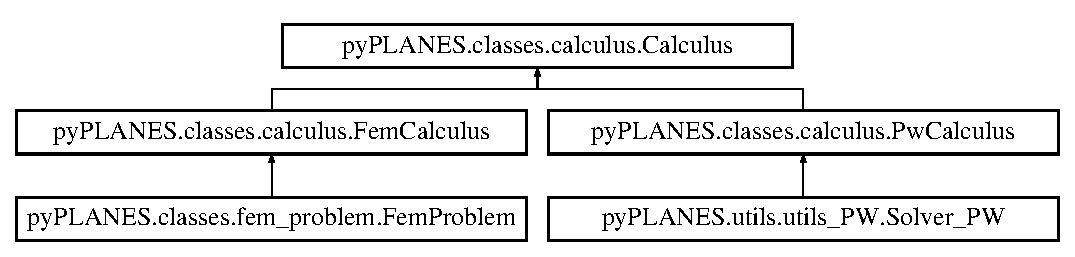
\includegraphics[height=3.000000cm]{classpy_p_l_a_n_e_s_1_1classes_1_1calculus_1_1_calculus}
\end{center}
\end{figure}
\subsection*{Public Member Functions}
\begin{DoxyCompactItemize}
\item 
\mbox{\Hypertarget{classpy_p_l_a_n_e_s_1_1classes_1_1calculus_1_1_calculus_a51fbbe939af1d9eaf6e9a36e34185d03}\label{classpy_p_l_a_n_e_s_1_1classes_1_1calculus_1_1_calculus_a51fbbe939af1d9eaf6e9a36e34185d03}} 
def {\bfseries \+\_\+\+\_\+init\+\_\+\+\_\+} (self, kwargs)
\item 
\mbox{\Hypertarget{classpy_p_l_a_n_e_s_1_1classes_1_1calculus_1_1_calculus_a887324122805b6064c66ae530f92ad44}\label{classpy_p_l_a_n_e_s_1_1classes_1_1calculus_1_1_calculus_a887324122805b6064c66ae530f92ad44}} 
def {\bfseries init\+\_\+vec\+\_\+frequencies} (self, frequency)
\item 
\mbox{\Hypertarget{classpy_p_l_a_n_e_s_1_1classes_1_1calculus_1_1_calculus_a939a153600c0a125e28a221911a03071}\label{classpy_p_l_a_n_e_s_1_1classes_1_1calculus_1_1_calculus_a939a153600c0a125e28a221911a03071}} 
def {\bfseries update\+\_\+frequency} (self, f)
\end{DoxyCompactItemize}
\subsection*{Public Attributes}
\begin{DoxyCompactItemize}
\item 
\mbox{\Hypertarget{classpy_p_l_a_n_e_s_1_1classes_1_1calculus_1_1_calculus_a46d44e93ffb105a61e167e1361651868}\label{classpy_p_l_a_n_e_s_1_1classes_1_1calculus_1_1_calculus_a46d44e93ffb105a61e167e1361651868}} 
{\bfseries frequencies}
\item 
\mbox{\Hypertarget{classpy_p_l_a_n_e_s_1_1classes_1_1calculus_1_1_calculus_a624c4aab758cc5e70d2c06b7197236ae}\label{classpy_p_l_a_n_e_s_1_1classes_1_1calculus_1_1_calculus_a624c4aab758cc5e70d2c06b7197236ae}} 
{\bfseries current\+\_\+frequency}
\item 
\mbox{\Hypertarget{classpy_p_l_a_n_e_s_1_1classes_1_1calculus_1_1_calculus_a4a4a24e9d093f492c757a9f6ddd18e4e}\label{classpy_p_l_a_n_e_s_1_1classes_1_1calculus_1_1_calculus_a4a4a24e9d093f492c757a9f6ddd18e4e}} 
{\bfseries omega}
\item 
\mbox{\Hypertarget{classpy_p_l_a_n_e_s_1_1classes_1_1calculus_1_1_calculus_ab2bf6be71b696b625e3fdfbdd6057e9e}\label{classpy_p_l_a_n_e_s_1_1classes_1_1calculus_1_1_calculus_ab2bf6be71b696b625e3fdfbdd6057e9e}} 
{\bfseries theta\+\_\+d}
\item 
\mbox{\Hypertarget{classpy_p_l_a_n_e_s_1_1classes_1_1calculus_1_1_calculus_a90897b5f71d8a1781979c41d89a8ce4f}\label{classpy_p_l_a_n_e_s_1_1classes_1_1calculus_1_1_calculus_a90897b5f71d8a1781979c41d89a8ce4f}} 
{\bfseries name\+\_\+project}
\item 
\mbox{\Hypertarget{classpy_p_l_a_n_e_s_1_1classes_1_1calculus_1_1_calculus_aeeef96d2c0922841fe1c6d9adcaf51cf}\label{classpy_p_l_a_n_e_s_1_1classes_1_1calculus_1_1_calculus_aeeef96d2c0922841fe1c6d9adcaf51cf}} 
{\bfseries outfiles\+\_\+directory}
\item 
\mbox{\Hypertarget{classpy_p_l_a_n_e_s_1_1classes_1_1calculus_1_1_calculus_afcad641a836beff4dfdbeef6c7055b0f}\label{classpy_p_l_a_n_e_s_1_1classes_1_1calculus_1_1_calculus_afcad641a836beff4dfdbeef6c7055b0f}} 
{\bfseries plot}
\end{DoxyCompactItemize}


The documentation for this class was generated from the following file\+:\begin{DoxyCompactItemize}
\item 
py\+P\+L\+A\+N\+E\+S/classes/calculus.\+py\end{DoxyCompactItemize}

\hypertarget{classpy_p_l_a_n_e_s_1_1gmsh_1_1write__geo__file_1_1_gmsh_1_1_circle}{}\section{py\+P\+L\+A\+N\+E\+S.\+gmsh.\+write\+\_\+geo\+\_\+file.\+Gmsh.\+Circle Class Reference}
\label{classpy_p_l_a_n_e_s_1_1gmsh_1_1write__geo__file_1_1_gmsh_1_1_circle}\index{py\+P\+L\+A\+N\+E\+S.\+gmsh.\+write\+\_\+geo\+\_\+file.\+Gmsh.\+Circle@{py\+P\+L\+A\+N\+E\+S.\+gmsh.\+write\+\_\+geo\+\_\+file.\+Gmsh.\+Circle}}
\subsection*{Public Member Functions}
\begin{DoxyCompactItemize}
\item 
\mbox{\Hypertarget{classpy_p_l_a_n_e_s_1_1gmsh_1_1write__geo__file_1_1_gmsh_1_1_circle_a0d91ac9d9c3d8ae0bb80fdb4dcf7cbe9}\label{classpy_p_l_a_n_e_s_1_1gmsh_1_1write__geo__file_1_1_gmsh_1_1_circle_a0d91ac9d9c3d8ae0bb80fdb4dcf7cbe9}} 
def {\bfseries \+\_\+\+\_\+init\+\_\+\+\_\+} (self, f, start\+\_\+tag, points)
\end{DoxyCompactItemize}
\subsection*{Public Attributes}
\begin{DoxyCompactItemize}
\item 
\mbox{\Hypertarget{classpy_p_l_a_n_e_s_1_1gmsh_1_1write__geo__file_1_1_gmsh_1_1_circle_a8457b824009b1c48a49f446bb9565160}\label{classpy_p_l_a_n_e_s_1_1gmsh_1_1write__geo__file_1_1_gmsh_1_1_circle_a8457b824009b1c48a49f446bb9565160}} 
{\bfseries typ}
\item 
\mbox{\Hypertarget{classpy_p_l_a_n_e_s_1_1gmsh_1_1write__geo__file_1_1_gmsh_1_1_circle_a151ae52a8b4f9842af85bb6a209aa134}\label{classpy_p_l_a_n_e_s_1_1gmsh_1_1write__geo__file_1_1_gmsh_1_1_circle_a151ae52a8b4f9842af85bb6a209aa134}} 
{\bfseries tag\+\_\+arcs}
\item 
\mbox{\Hypertarget{classpy_p_l_a_n_e_s_1_1gmsh_1_1write__geo__file_1_1_gmsh_1_1_circle_ac540be9bc92c1c0f986c5524878a69c0}\label{classpy_p_l_a_n_e_s_1_1gmsh_1_1write__geo__file_1_1_gmsh_1_1_circle_ac540be9bc92c1c0f986c5524878a69c0}} 
{\bfseries tag}
\end{DoxyCompactItemize}


The documentation for this class was generated from the following file\+:\begin{DoxyCompactItemize}
\item 
py\+P\+L\+A\+N\+E\+S/gmsh/write\+\_\+geo\+\_\+file.\+py\end{DoxyCompactItemize}

\hypertarget{classpy_p_l_a_n_e_s_1_1classes_1_1fem__classes_1_1_edge}{}\section{py\+P\+L\+A\+N\+E\+S.\+classes.\+fem\+\_\+classes.\+Edge Class Reference}
\label{classpy_p_l_a_n_e_s_1_1classes_1_1fem__classes_1_1_edge}\index{py\+P\+L\+A\+N\+E\+S.\+classes.\+fem\+\_\+classes.\+Edge@{py\+P\+L\+A\+N\+E\+S.\+classes.\+fem\+\_\+classes.\+Edge}}
\subsection*{Public Member Functions}
\begin{DoxyCompactItemize}
\item 
\mbox{\Hypertarget{classpy_p_l_a_n_e_s_1_1classes_1_1fem__classes_1_1_edge_a530f7d59969ae0b371903b5ac0354587}\label{classpy_p_l_a_n_e_s_1_1classes_1_1fem__classes_1_1_edge_a530f7d59969ae0b371903b5ac0354587}} 
def {\bfseries \+\_\+\+\_\+init\+\_\+\+\_\+} (self, tag, vertices, element, order)
\item 
\mbox{\Hypertarget{classpy_p_l_a_n_e_s_1_1classes_1_1fem__classes_1_1_edge_a8547d3032b0510e1565b008f68786b70}\label{classpy_p_l_a_n_e_s_1_1classes_1_1fem__classes_1_1_edge_a8547d3032b0510e1565b008f68786b70}} 
def {\bfseries center} (self)
\item 
\mbox{\Hypertarget{classpy_p_l_a_n_e_s_1_1classes_1_1fem__classes_1_1_edge_a64358a0be626f48dcbd46be2fff2e393}\label{classpy_p_l_a_n_e_s_1_1classes_1_1fem__classes_1_1_edge_a64358a0be626f48dcbd46be2fff2e393}} 
def {\bfseries \+\_\+\+\_\+str\+\_\+\+\_\+} (self)
\end{DoxyCompactItemize}
\subsection*{Public Attributes}
\begin{DoxyCompactItemize}
\item 
\mbox{\Hypertarget{classpy_p_l_a_n_e_s_1_1classes_1_1fem__classes_1_1_edge_a9785ce0b437f7ff68dc52308fb424e93}\label{classpy_p_l_a_n_e_s_1_1classes_1_1fem__classes_1_1_edge_a9785ce0b437f7ff68dc52308fb424e93}} 
{\bfseries tag}
\item 
\mbox{\Hypertarget{classpy_p_l_a_n_e_s_1_1classes_1_1fem__classes_1_1_edge_a3355efc1f35654a5d7ff704d22ed38da}\label{classpy_p_l_a_n_e_s_1_1classes_1_1fem__classes_1_1_edge_a3355efc1f35654a5d7ff704d22ed38da}} 
{\bfseries vertices}
\item 
\mbox{\Hypertarget{classpy_p_l_a_n_e_s_1_1classes_1_1fem__classes_1_1_edge_ace32c6f6a790faf9889e7ccb2529ebbc}\label{classpy_p_l_a_n_e_s_1_1classes_1_1fem__classes_1_1_edge_ace32c6f6a790faf9889e7ccb2529ebbc}} 
{\bfseries elements}
\item 
\mbox{\Hypertarget{classpy_p_l_a_n_e_s_1_1classes_1_1fem__classes_1_1_edge_a9bcdaeb331419288b7603e3500798bc0}\label{classpy_p_l_a_n_e_s_1_1classes_1_1fem__classes_1_1_edge_a9bcdaeb331419288b7603e3500798bc0}} 
{\bfseries order}
\item 
\mbox{\Hypertarget{classpy_p_l_a_n_e_s_1_1classes_1_1fem__classes_1_1_edge_af0bb7ffc3bb8a4e5aaeed266ad18a221}\label{classpy_p_l_a_n_e_s_1_1classes_1_1fem__classes_1_1_edge_af0bb7ffc3bb8a4e5aaeed266ad18a221}} 
{\bfseries dofs}
\item 
\mbox{\Hypertarget{classpy_p_l_a_n_e_s_1_1classes_1_1fem__classes_1_1_edge_aa7cc9cb266b94964101fd26c89773dbb}\label{classpy_p_l_a_n_e_s_1_1classes_1_1fem__classes_1_1_edge_aa7cc9cb266b94964101fd26c89773dbb}} 
{\bfseries sol}
\end{DoxyCompactItemize}


\subsection{Detailed Description}
\begin{DoxyVerb}TODO \end{DoxyVerb}
 

The documentation for this class was generated from the following file\+:\begin{DoxyCompactItemize}
\item 
py\+P\+L\+A\+N\+E\+S/classes/fem\+\_\+classes.\+py\end{DoxyCompactItemize}

\hypertarget{classpy_p_l_a_n_e_s_1_1classes_1_1entity__classes_1_1_elastic_fem}{}\section{py\+P\+L\+A\+N\+E\+S.\+classes.\+entity\+\_\+classes.\+Elastic\+Fem Class Reference}
\label{classpy_p_l_a_n_e_s_1_1classes_1_1entity__classes_1_1_elastic_fem}\index{py\+P\+L\+A\+N\+E\+S.\+classes.\+entity\+\_\+classes.\+Elastic\+Fem@{py\+P\+L\+A\+N\+E\+S.\+classes.\+entity\+\_\+classes.\+Elastic\+Fem}}
Inheritance diagram for py\+P\+L\+A\+N\+E\+S.\+classes.\+entity\+\_\+classes.\+Elastic\+Fem\+:\begin{figure}[H]
\begin{center}
\leavevmode
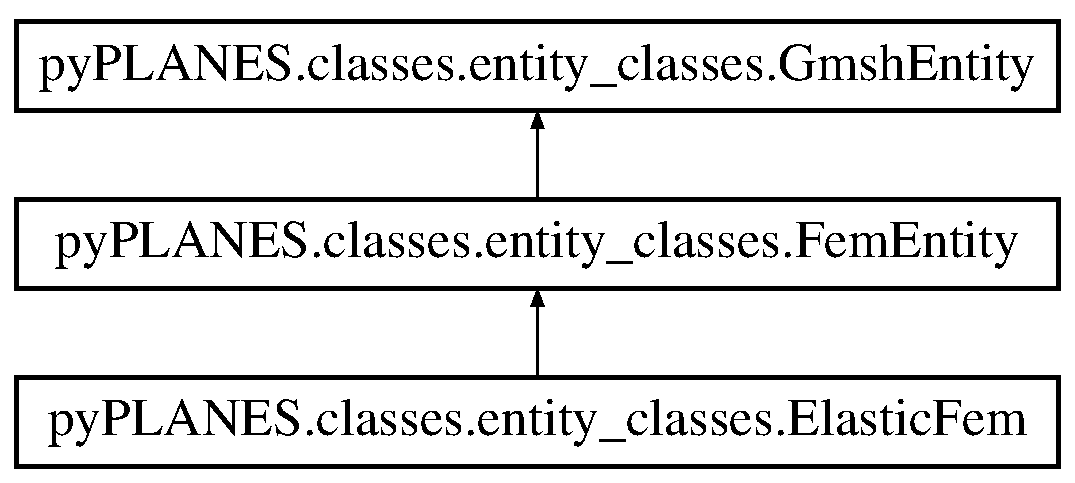
\includegraphics[height=3.000000cm]{classpy_p_l_a_n_e_s_1_1classes_1_1entity__classes_1_1_elastic_fem}
\end{center}
\end{figure}
\subsection*{Public Member Functions}
\begin{DoxyCompactItemize}
\item 
\mbox{\Hypertarget{classpy_p_l_a_n_e_s_1_1classes_1_1entity__classes_1_1_elastic_fem_a4cb7e815035fed9eccaf5cecc2d53933}\label{classpy_p_l_a_n_e_s_1_1classes_1_1entity__classes_1_1_elastic_fem_a4cb7e815035fed9eccaf5cecc2d53933}} 
def {\bfseries \+\_\+\+\_\+init\+\_\+\+\_\+} (self, kwargs)
\item 
\mbox{\Hypertarget{classpy_p_l_a_n_e_s_1_1classes_1_1entity__classes_1_1_elastic_fem_a30482821d48e9c80549d0cfa0a4158d8}\label{classpy_p_l_a_n_e_s_1_1classes_1_1entity__classes_1_1_elastic_fem_a30482821d48e9c80549d0cfa0a4158d8}} 
def {\bfseries \+\_\+\+\_\+str\+\_\+\+\_\+} (self)
\item 
\mbox{\Hypertarget{classpy_p_l_a_n_e_s_1_1classes_1_1entity__classes_1_1_elastic_fem_aa45ec0d99df75ecfeadaa1d43a9d231d}\label{classpy_p_l_a_n_e_s_1_1classes_1_1entity__classes_1_1_elastic_fem_aa45ec0d99df75ecfeadaa1d43a9d231d}} 
def {\bfseries update\+\_\+frequency} (self, omega)
\item 
\mbox{\Hypertarget{classpy_p_l_a_n_e_s_1_1classes_1_1entity__classes_1_1_elastic_fem_aabcf6cb460abbc21b17423562ce91530}\label{classpy_p_l_a_n_e_s_1_1classes_1_1entity__classes_1_1_elastic_fem_aabcf6cb460abbc21b17423562ce91530}} 
def {\bfseries elementary\+\_\+matrices} (self, \+\_\+el)
\item 
\mbox{\Hypertarget{classpy_p_l_a_n_e_s_1_1classes_1_1entity__classes_1_1_elastic_fem_a24e1a6c806d8d5f5e38dbec96249d226}\label{classpy_p_l_a_n_e_s_1_1classes_1_1entity__classes_1_1_elastic_fem_a24e1a6c806d8d5f5e38dbec96249d226}} 
def {\bfseries append\+\_\+linear\+\_\+system} (self, omega)
\end{DoxyCompactItemize}
\subsection*{Public Attributes}
\begin{DoxyCompactItemize}
\item 
\mbox{\Hypertarget{classpy_p_l_a_n_e_s_1_1classes_1_1entity__classes_1_1_elastic_fem_a64da06452fee91e2520768863f1bc815}\label{classpy_p_l_a_n_e_s_1_1classes_1_1entity__classes_1_1_elastic_fem_a64da06452fee91e2520768863f1bc815}} 
{\bfseries mat}
\end{DoxyCompactItemize}


The documentation for this class was generated from the following file\+:\begin{DoxyCompactItemize}
\item 
py\+P\+L\+A\+N\+E\+S/classes/entity\+\_\+classes.\+py\end{DoxyCompactItemize}

\hypertarget{classpy_p_l_a_n_e_s_1_1classes_1_1fem__classes_1_1_element}{}\section{py\+P\+L\+A\+N\+E\+S.\+classes.\+fem\+\_\+classes.\+Element Class Reference}
\label{classpy_p_l_a_n_e_s_1_1classes_1_1fem__classes_1_1_element}\index{py\+P\+L\+A\+N\+E\+S.\+classes.\+fem\+\_\+classes.\+Element@{py\+P\+L\+A\+N\+E\+S.\+classes.\+fem\+\_\+classes.\+Element}}
\subsection*{Public Member Functions}
\begin{DoxyCompactItemize}
\item 
\mbox{\Hypertarget{classpy_p_l_a_n_e_s_1_1classes_1_1fem__classes_1_1_element_a97e569455738d42e030df2a6b1f17911}\label{classpy_p_l_a_n_e_s_1_1classes_1_1fem__classes_1_1_element_a97e569455738d42e030df2a6b1f17911}} 
def {\bfseries \+\_\+\+\_\+init\+\_\+\+\_\+} (self, typ, tag, vertices, reference\+\_\+element)
\item 
\mbox{\Hypertarget{classpy_p_l_a_n_e_s_1_1classes_1_1fem__classes_1_1_element_afe6e7565839bf666a73899ca29cdb297}\label{classpy_p_l_a_n_e_s_1_1classes_1_1fem__classes_1_1_element_afe6e7565839bf666a73899ca29cdb297}} 
def {\bfseries \+\_\+\+\_\+str\+\_\+\+\_\+} (self)
\item 
def \mbox{\hyperlink{classpy_p_l_a_n_e_s_1_1classes_1_1fem__classes_1_1_element_a1ebd212c04bb221d14aecbe36458dfda}{get\+\_\+coordinates}} (self)
\item 
def \mbox{\hyperlink{classpy_p_l_a_n_e_s_1_1classes_1_1fem__classes_1_1_element_ace2dc657fe00985caf3aebda50d27fb9}{get\+\_\+center}} (self)
\item 
\mbox{\Hypertarget{classpy_p_l_a_n_e_s_1_1classes_1_1fem__classes_1_1_element_a77c10e9d25310d022a9a1b1276d2b017}\label{classpy_p_l_a_n_e_s_1_1classes_1_1fem__classes_1_1_element_a77c10e9d25310d022a9a1b1276d2b017}} 
def {\bfseries display\+\_\+sol} (self, field)
\item 
\mbox{\Hypertarget{classpy_p_l_a_n_e_s_1_1classes_1_1fem__classes_1_1_element_a065f56d42ea88e316e7001e321abf11f}\label{classpy_p_l_a_n_e_s_1_1classes_1_1fem__classes_1_1_element_a065f56d42ea88e316e7001e321abf11f}} 
def {\bfseries elementary\+\_\+matrices} (self)
\end{DoxyCompactItemize}
\subsection*{Public Attributes}
\begin{DoxyCompactItemize}
\item 
\mbox{\Hypertarget{classpy_p_l_a_n_e_s_1_1classes_1_1fem__classes_1_1_element_add63fc0a53f859ecf986f6a9281445e8}\label{classpy_p_l_a_n_e_s_1_1classes_1_1fem__classes_1_1_element_add63fc0a53f859ecf986f6a9281445e8}} 
{\bfseries typ}
\item 
\mbox{\Hypertarget{classpy_p_l_a_n_e_s_1_1classes_1_1fem__classes_1_1_element_aa8b87a18b57ebdf5d5363d0a7479b28a}\label{classpy_p_l_a_n_e_s_1_1classes_1_1fem__classes_1_1_element_aa8b87a18b57ebdf5d5363d0a7479b28a}} 
{\bfseries tag}
\item 
\mbox{\Hypertarget{classpy_p_l_a_n_e_s_1_1classes_1_1fem__classes_1_1_element_a455e523266df3e3f54a5d805abd5b428}\label{classpy_p_l_a_n_e_s_1_1classes_1_1fem__classes_1_1_element_a455e523266df3e3f54a5d805abd5b428}} 
{\bfseries vertices}
\item 
\mbox{\Hypertarget{classpy_p_l_a_n_e_s_1_1classes_1_1fem__classes_1_1_element_a5bb05e628beab636ccd32d6414604b1b}\label{classpy_p_l_a_n_e_s_1_1classes_1_1fem__classes_1_1_element_a5bb05e628beab636ccd32d6414604b1b}} 
{\bfseries reference\+\_\+element}
\item 
\mbox{\Hypertarget{classpy_p_l_a_n_e_s_1_1classes_1_1fem__classes_1_1_element_a7b52dd3395d7331aea3b6eb5abfa1a07}\label{classpy_p_l_a_n_e_s_1_1classes_1_1fem__classes_1_1_element_a7b52dd3395d7331aea3b6eb5abfa1a07}} 
{\bfseries dofs}
\item 
\mbox{\Hypertarget{classpy_p_l_a_n_e_s_1_1classes_1_1fem__classes_1_1_element_a26c8e5ea7fa9a76972b4838414814e22}\label{classpy_p_l_a_n_e_s_1_1classes_1_1fem__classes_1_1_element_a26c8e5ea7fa9a76972b4838414814e22}} 
{\bfseries edges}
\item 
\mbox{\Hypertarget{classpy_p_l_a_n_e_s_1_1classes_1_1fem__classes_1_1_element_a08c47d843c0211e025a4238a10716ed8}\label{classpy_p_l_a_n_e_s_1_1classes_1_1fem__classes_1_1_element_a08c47d843c0211e025a4238a10716ed8}} 
{\bfseries edges\+\_\+orientation}
\item 
\mbox{\Hypertarget{classpy_p_l_a_n_e_s_1_1classes_1_1fem__classes_1_1_element_ab5c68cab5a6b28c24a572fa1351b2674}\label{classpy_p_l_a_n_e_s_1_1classes_1_1fem__classes_1_1_element_ab5c68cab5a6b28c24a572fa1351b2674}} 
{\bfseries nb\+\_\+edges}
\item 
\mbox{\Hypertarget{classpy_p_l_a_n_e_s_1_1classes_1_1fem__classes_1_1_element_a0d20208388270c6b447e84d3ebae6033}\label{classpy_p_l_a_n_e_s_1_1classes_1_1fem__classes_1_1_element_a0d20208388270c6b447e84d3ebae6033}} 
{\bfseries faces}
\item 
\mbox{\Hypertarget{classpy_p_l_a_n_e_s_1_1classes_1_1fem__classes_1_1_element_acd4060a134ed5c4fb3800c1d6fb479c5}\label{classpy_p_l_a_n_e_s_1_1classes_1_1fem__classes_1_1_element_acd4060a134ed5c4fb3800c1d6fb479c5}} 
{\bfseries faces\+\_\+orientation}
\end{DoxyCompactItemize}


\subsection{Detailed Description}
\begin{DoxyVerb}Element of pyPLANES

Parameters:
-----------
typ : int
    GMSH type of the element

coorde : numpy array
    Array of nodes coordinates (dim = 3x nb vertices )

Ref_Elem : Reference Element

Returns:
------------------------
None

Attributes :
------------------------

edges : List of edge instances associated to the element

faces : List of face instances associated to the element (optional)

bubbles : List of bubble instances associated to the element (optional)\end{DoxyVerb}
 

\subsection{Member Function Documentation}
\mbox{\Hypertarget{classpy_p_l_a_n_e_s_1_1classes_1_1fem__classes_1_1_element_ace2dc657fe00985caf3aebda50d27fb9}\label{classpy_p_l_a_n_e_s_1_1classes_1_1fem__classes_1_1_element_ace2dc657fe00985caf3aebda50d27fb9}} 
\index{py\+P\+L\+A\+N\+E\+S\+::classes\+::fem\+\_\+classes\+::\+Element@{py\+P\+L\+A\+N\+E\+S\+::classes\+::fem\+\_\+classes\+::\+Element}!get\+\_\+center@{get\+\_\+center}}
\index{get\+\_\+center@{get\+\_\+center}!py\+P\+L\+A\+N\+E\+S\+::classes\+::fem\+\_\+classes\+::\+Element@{py\+P\+L\+A\+N\+E\+S\+::classes\+::fem\+\_\+classes\+::\+Element}}
\subsubsection{\texorpdfstring{get\+\_\+center()}{get\_center()}}
{\footnotesize\ttfamily def py\+P\+L\+A\+N\+E\+S.\+classes.\+fem\+\_\+classes.\+Element.\+get\+\_\+center (\begin{DoxyParamCaption}\item[{}]{self }\end{DoxyParamCaption})}

\begin{DoxyVerb}Method that gives the center of the element\end{DoxyVerb}
 \mbox{\Hypertarget{classpy_p_l_a_n_e_s_1_1classes_1_1fem__classes_1_1_element_a1ebd212c04bb221d14aecbe36458dfda}\label{classpy_p_l_a_n_e_s_1_1classes_1_1fem__classes_1_1_element_a1ebd212c04bb221d14aecbe36458dfda}} 
\index{py\+P\+L\+A\+N\+E\+S\+::classes\+::fem\+\_\+classes\+::\+Element@{py\+P\+L\+A\+N\+E\+S\+::classes\+::fem\+\_\+classes\+::\+Element}!get\+\_\+coordinates@{get\+\_\+coordinates}}
\index{get\+\_\+coordinates@{get\+\_\+coordinates}!py\+P\+L\+A\+N\+E\+S\+::classes\+::fem\+\_\+classes\+::\+Element@{py\+P\+L\+A\+N\+E\+S\+::classes\+::fem\+\_\+classes\+::\+Element}}
\subsubsection{\texorpdfstring{get\+\_\+coordinates()}{get\_coordinates()}}
{\footnotesize\ttfamily def py\+P\+L\+A\+N\+E\+S.\+classes.\+fem\+\_\+classes.\+Element.\+get\+\_\+coordinates (\begin{DoxyParamCaption}\item[{}]{self }\end{DoxyParamCaption})}

\begin{DoxyVerb}Method that gives the geometrical coordinates of the element\end{DoxyVerb}
 

The documentation for this class was generated from the following file\+:\begin{DoxyCompactItemize}
\item 
py\+P\+L\+A\+N\+E\+S/classes/fem\+\_\+classes.\+py\end{DoxyCompactItemize}

\hypertarget{classpy_p_l_a_n_e_s_1_1classes_1_1fem__classes_1_1_face}{}\section{py\+P\+L\+A\+N\+E\+S.\+classes.\+fem\+\_\+classes.\+Face Class Reference}
\label{classpy_p_l_a_n_e_s_1_1classes_1_1fem__classes_1_1_face}\index{py\+P\+L\+A\+N\+E\+S.\+classes.\+fem\+\_\+classes.\+Face@{py\+P\+L\+A\+N\+E\+S.\+classes.\+fem\+\_\+classes.\+Face}}
\subsection*{Public Member Functions}
\begin{DoxyCompactItemize}
\item 
\mbox{\Hypertarget{classpy_p_l_a_n_e_s_1_1classes_1_1fem__classes_1_1_face_af57837060ba996945d520ddad2761862}\label{classpy_p_l_a_n_e_s_1_1classes_1_1fem__classes_1_1_face_af57837060ba996945d520ddad2761862}} 
def {\bfseries \+\_\+\+\_\+init\+\_\+\+\_\+} (self, tag, vertices, element, order)
\item 
\mbox{\Hypertarget{classpy_p_l_a_n_e_s_1_1classes_1_1fem__classes_1_1_face_a33e3e3d15e9420bf57387f0334580455}\label{classpy_p_l_a_n_e_s_1_1classes_1_1fem__classes_1_1_face_a33e3e3d15e9420bf57387f0334580455}} 
def {\bfseries \+\_\+\+\_\+str\+\_\+\+\_\+} (self)
\end{DoxyCompactItemize}
\subsection*{Public Attributes}
\begin{DoxyCompactItemize}
\item 
\mbox{\Hypertarget{classpy_p_l_a_n_e_s_1_1classes_1_1fem__classes_1_1_face_a414d49b99bd4c544739e1ec81b8dd9a9}\label{classpy_p_l_a_n_e_s_1_1classes_1_1fem__classes_1_1_face_a414d49b99bd4c544739e1ec81b8dd9a9}} 
{\bfseries tag}
\item 
\mbox{\Hypertarget{classpy_p_l_a_n_e_s_1_1classes_1_1fem__classes_1_1_face_a41ea53ceb43a43f52dcf54804114b7df}\label{classpy_p_l_a_n_e_s_1_1classes_1_1fem__classes_1_1_face_a41ea53ceb43a43f52dcf54804114b7df}} 
{\bfseries vertices}
\item 
\mbox{\Hypertarget{classpy_p_l_a_n_e_s_1_1classes_1_1fem__classes_1_1_face_a808f1904143f264c7344cc03d6bb3327}\label{classpy_p_l_a_n_e_s_1_1classes_1_1fem__classes_1_1_face_a808f1904143f264c7344cc03d6bb3327}} 
{\bfseries elements}
\item 
\mbox{\Hypertarget{classpy_p_l_a_n_e_s_1_1classes_1_1fem__classes_1_1_face_a6dd7fbf08694fc06a32146293d7ccf8c}\label{classpy_p_l_a_n_e_s_1_1classes_1_1fem__classes_1_1_face_a6dd7fbf08694fc06a32146293d7ccf8c}} 
{\bfseries order}
\item 
\mbox{\Hypertarget{classpy_p_l_a_n_e_s_1_1classes_1_1fem__classes_1_1_face_ababe401581453db1ecf5bb1de6b9fb2d}\label{classpy_p_l_a_n_e_s_1_1classes_1_1fem__classes_1_1_face_ababe401581453db1ecf5bb1de6b9fb2d}} 
{\bfseries dofs}
\item 
\mbox{\Hypertarget{classpy_p_l_a_n_e_s_1_1classes_1_1fem__classes_1_1_face_a17c9de278c931b618526cb84ab044549}\label{classpy_p_l_a_n_e_s_1_1classes_1_1fem__classes_1_1_face_a17c9de278c931b618526cb84ab044549}} 
{\bfseries sol}
\end{DoxyCompactItemize}


\subsection{Detailed Description}
\begin{DoxyVerb}Class Face \end{DoxyVerb}
 

The documentation for this class was generated from the following file\+:\begin{DoxyCompactItemize}
\item 
py\+P\+L\+A\+N\+E\+S/classes/fem\+\_\+classes.\+py\end{DoxyCompactItemize}

\hypertarget{classpy_p_l_a_n_e_s_1_1classes_1_1calculus_1_1_fem_calculus}{}\section{py\+P\+L\+A\+N\+E\+S.\+classes.\+calculus.\+Fem\+Calculus Class Reference}
\label{classpy_p_l_a_n_e_s_1_1classes_1_1calculus_1_1_fem_calculus}\index{py\+P\+L\+A\+N\+E\+S.\+classes.\+calculus.\+Fem\+Calculus@{py\+P\+L\+A\+N\+E\+S.\+classes.\+calculus.\+Fem\+Calculus}}
Inheritance diagram for py\+P\+L\+A\+N\+E\+S.\+classes.\+calculus.\+Fem\+Calculus\+:\begin{figure}[H]
\begin{center}
\leavevmode
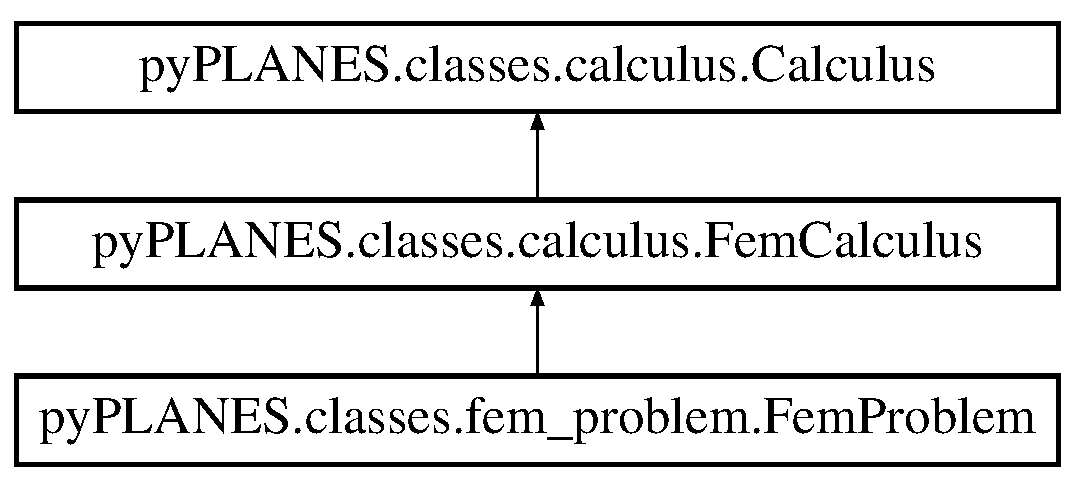
\includegraphics[height=3.000000cm]{classpy_p_l_a_n_e_s_1_1classes_1_1calculus_1_1_fem_calculus}
\end{center}
\end{figure}
\subsection*{Public Member Functions}
\begin{DoxyCompactItemize}
\item 
\mbox{\Hypertarget{classpy_p_l_a_n_e_s_1_1classes_1_1calculus_1_1_fem_calculus_aa0f7fb6a02400e5ac425b41e8b9463f9}\label{classpy_p_l_a_n_e_s_1_1classes_1_1calculus_1_1_fem_calculus_aa0f7fb6a02400e5ac425b41e8b9463f9}} 
def {\bfseries \+\_\+\+\_\+init\+\_\+\+\_\+} (self, kwargs)
\item 
\mbox{\Hypertarget{classpy_p_l_a_n_e_s_1_1classes_1_1calculus_1_1_fem_calculus_ab129ddbbce45f69afc2422acb4edbc0a}\label{classpy_p_l_a_n_e_s_1_1classes_1_1calculus_1_1_fem_calculus_ab129ddbbce45f69afc2422acb4edbc0a}} 
def {\bfseries update\+\_\+frequency} (self, f)
\end{DoxyCompactItemize}
\subsection*{Public Attributes}
\begin{DoxyCompactItemize}
\item 
\mbox{\Hypertarget{classpy_p_l_a_n_e_s_1_1classes_1_1calculus_1_1_fem_calculus_acda274e6ceb0d3dbb0c3922d3e06d758}\label{classpy_p_l_a_n_e_s_1_1classes_1_1calculus_1_1_fem_calculus_acda274e6ceb0d3dbb0c3922d3e06d758}} 
{\bfseries out\+\_\+file}
\item 
\mbox{\Hypertarget{classpy_p_l_a_n_e_s_1_1classes_1_1calculus_1_1_fem_calculus_ab0dfe9d301fe821d0b9f2fa3617159f5}\label{classpy_p_l_a_n_e_s_1_1classes_1_1calculus_1_1_fem_calculus_ab0dfe9d301fe821d0b9f2fa3617159f5}} 
{\bfseries info\+\_\+file}
\item 
\mbox{\Hypertarget{classpy_p_l_a_n_e_s_1_1classes_1_1calculus_1_1_fem_calculus_ae37ed144b8ed36cca4d7105eba4c115c}\label{classpy_p_l_a_n_e_s_1_1classes_1_1calculus_1_1_fem_calculus_ae37ed144b8ed36cca4d7105eba4c115c}} 
{\bfseries F\+\_\+v}
\item 
\mbox{\Hypertarget{classpy_p_l_a_n_e_s_1_1classes_1_1calculus_1_1_fem_calculus_adcccdd98990d5d803e91af47bcd2afd3}\label{classpy_p_l_a_n_e_s_1_1classes_1_1calculus_1_1_fem_calculus_adcccdd98990d5d803e91af47bcd2afd3}} 
{\bfseries A\+\_\+v}
\item 
\mbox{\Hypertarget{classpy_p_l_a_n_e_s_1_1classes_1_1calculus_1_1_fem_calculus_a1bd9998dd917204e4feb2aa3c4d6cd37}\label{classpy_p_l_a_n_e_s_1_1classes_1_1calculus_1_1_fem_calculus_a1bd9998dd917204e4feb2aa3c4d6cd37}} 
{\bfseries A\+\_\+v\+\_\+c}
\item 
\mbox{\Hypertarget{classpy_p_l_a_n_e_s_1_1classes_1_1calculus_1_1_fem_calculus_ab6d5dac92d46779cfe7f6d441dd66358}\label{classpy_p_l_a_n_e_s_1_1classes_1_1calculus_1_1_fem_calculus_ab6d5dac92d46779cfe7f6d441dd66358}} 
{\bfseries T\+\_\+v}
\item 
\mbox{\Hypertarget{classpy_p_l_a_n_e_s_1_1classes_1_1calculus_1_1_fem_calculus_a24da7bfc5fdaa6b1e4bc37e13bcbc56c}\label{classpy_p_l_a_n_e_s_1_1classes_1_1calculus_1_1_fem_calculus_a24da7bfc5fdaa6b1e4bc37e13bcbc56c}} 
{\bfseries abs}
\item 
\mbox{\Hypertarget{classpy_p_l_a_n_e_s_1_1classes_1_1calculus_1_1_fem_calculus_a4bc4e2e905f1d48069ef1f53b072976f}\label{classpy_p_l_a_n_e_s_1_1classes_1_1calculus_1_1_fem_calculus_a4bc4e2e905f1d48069ef1f53b072976f}} 
{\bfseries kx}
\item 
\mbox{\Hypertarget{classpy_p_l_a_n_e_s_1_1classes_1_1calculus_1_1_fem_calculus_ad77e2a7f452dd7d3bb20cc61e531abb5}\label{classpy_p_l_a_n_e_s_1_1classes_1_1calculus_1_1_fem_calculus_ad77e2a7f452dd7d3bb20cc61e531abb5}} 
{\bfseries ky}
\item 
\mbox{\Hypertarget{classpy_p_l_a_n_e_s_1_1classes_1_1calculus_1_1_fem_calculus_a72e4423ba0df40c9a93e5d816660e084}\label{classpy_p_l_a_n_e_s_1_1classes_1_1calculus_1_1_fem_calculus_a72e4423ba0df40c9a93e5d816660e084}} 
{\bfseries delta\+\_\+periodicity}
\item 
\mbox{\Hypertarget{classpy_p_l_a_n_e_s_1_1classes_1_1calculus_1_1_fem_calculus_a7b84fa22a90d345b021cde23817bfe5f}\label{classpy_p_l_a_n_e_s_1_1classes_1_1calculus_1_1_fem_calculus_a7b84fa22a90d345b021cde23817bfe5f}} 
{\bfseries nb\+\_\+dofs}
\end{DoxyCompactItemize}


The documentation for this class was generated from the following file\+:\begin{DoxyCompactItemize}
\item 
py\+P\+L\+A\+N\+E\+S/classes/calculus.\+py\end{DoxyCompactItemize}

\hypertarget{classpy_p_l_a_n_e_s_1_1classes_1_1entity__classes_1_1_fem_entity}{}\section{py\+P\+L\+A\+N\+E\+S.\+classes.\+entity\+\_\+classes.\+Fem\+Entity Class Reference}
\label{classpy_p_l_a_n_e_s_1_1classes_1_1entity__classes_1_1_fem_entity}\index{py\+P\+L\+A\+N\+E\+S.\+classes.\+entity\+\_\+classes.\+Fem\+Entity@{py\+P\+L\+A\+N\+E\+S.\+classes.\+entity\+\_\+classes.\+Fem\+Entity}}
Inheritance diagram for py\+P\+L\+A\+N\+E\+S.\+classes.\+entity\+\_\+classes.\+Fem\+Entity\+:\begin{figure}[H]
\begin{center}
\leavevmode
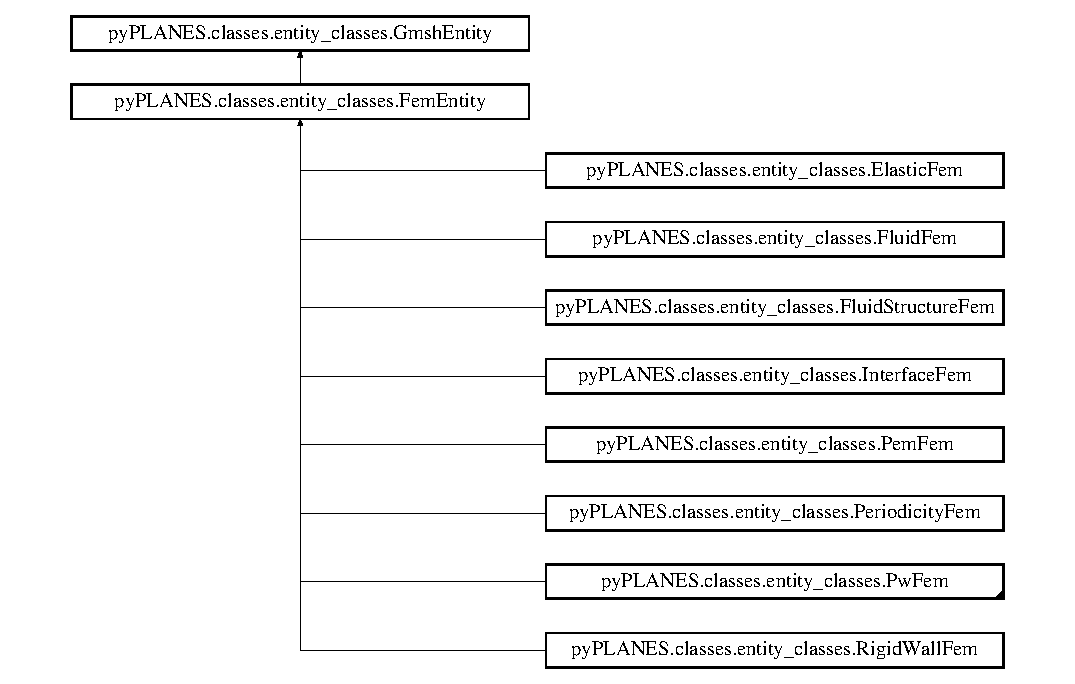
\includegraphics[height=8.750000cm]{classpy_p_l_a_n_e_s_1_1classes_1_1entity__classes_1_1_fem_entity}
\end{center}
\end{figure}
\subsection*{Public Member Functions}
\begin{DoxyCompactItemize}
\item 
\mbox{\Hypertarget{classpy_p_l_a_n_e_s_1_1classes_1_1entity__classes_1_1_fem_entity_aed59e4231f2d4d63d98ec9c4212cb941}\label{classpy_p_l_a_n_e_s_1_1classes_1_1entity__classes_1_1_fem_entity_aed59e4231f2d4d63d98ec9c4212cb941}} 
def {\bfseries \+\_\+\+\_\+init\+\_\+\+\_\+} (self, kwargs)
\item 
\mbox{\Hypertarget{classpy_p_l_a_n_e_s_1_1classes_1_1entity__classes_1_1_fem_entity_a06d9672473dd9ed9de4190df015884de}\label{classpy_p_l_a_n_e_s_1_1classes_1_1entity__classes_1_1_fem_entity_a06d9672473dd9ed9de4190df015884de}} 
def {\bfseries \+\_\+\+\_\+str\+\_\+\+\_\+} (self)
\item 
\mbox{\Hypertarget{classpy_p_l_a_n_e_s_1_1classes_1_1entity__classes_1_1_fem_entity_a808461e72bfff3ead5c2b43517d24d4c}\label{classpy_p_l_a_n_e_s_1_1classes_1_1entity__classes_1_1_fem_entity_a808461e72bfff3ead5c2b43517d24d4c}} 
def {\bfseries condensation} (self, omega)
\item 
\mbox{\Hypertarget{classpy_p_l_a_n_e_s_1_1classes_1_1entity__classes_1_1_fem_entity_a812ccc54dedfb622d20b4d5f6bc82848}\label{classpy_p_l_a_n_e_s_1_1classes_1_1entity__classes_1_1_fem_entity_a812ccc54dedfb622d20b4d5f6bc82848}} 
def {\bfseries update\+\_\+frequency} (self, omega)
\item 
\mbox{\Hypertarget{classpy_p_l_a_n_e_s_1_1classes_1_1entity__classes_1_1_fem_entity_a357347bfcc5dacbaf8faae0ea4e95cd8}\label{classpy_p_l_a_n_e_s_1_1classes_1_1entity__classes_1_1_fem_entity_a357347bfcc5dacbaf8faae0ea4e95cd8}} 
def {\bfseries elementary\+\_\+matrices} (self, \+\_\+elem)
\item 
\mbox{\Hypertarget{classpy_p_l_a_n_e_s_1_1classes_1_1entity__classes_1_1_fem_entity_ae901dea40e4ba37e5c473a842313a9ee}\label{classpy_p_l_a_n_e_s_1_1classes_1_1entity__classes_1_1_fem_entity_ae901dea40e4ba37e5c473a842313a9ee}} 
def {\bfseries append\+\_\+linear\+\_\+system} (self, omega)
\item 
\mbox{\Hypertarget{classpy_p_l_a_n_e_s_1_1classes_1_1entity__classes_1_1_fem_entity_aef9eed821fd92ee2cab0d986fe100eaf}\label{classpy_p_l_a_n_e_s_1_1classes_1_1entity__classes_1_1_fem_entity_aef9eed821fd92ee2cab0d986fe100eaf}} 
def {\bfseries link\+\_\+elem} (self, n)
\end{DoxyCompactItemize}
\subsection*{Public Attributes}
\begin{DoxyCompactItemize}
\item 
\mbox{\Hypertarget{classpy_p_l_a_n_e_s_1_1classes_1_1entity__classes_1_1_fem_entity_adcd9fcbc4261dd545bd17f60ddb63bf6}\label{classpy_p_l_a_n_e_s_1_1classes_1_1entity__classes_1_1_fem_entity_adcd9fcbc4261dd545bd17f60ddb63bf6}} 
{\bfseries order}
\item 
\mbox{\Hypertarget{classpy_p_l_a_n_e_s_1_1classes_1_1entity__classes_1_1_fem_entity_a9ede6ff44775d1cb2a2f93c6d3c03103}\label{classpy_p_l_a_n_e_s_1_1classes_1_1entity__classes_1_1_fem_entity_a9ede6ff44775d1cb2a2f93c6d3c03103}} 
{\bfseries elements}
\end{DoxyCompactItemize}


The documentation for this class was generated from the following file\+:\begin{DoxyCompactItemize}
\item 
py\+P\+L\+A\+N\+E\+S/classes/entity\+\_\+classes.\+py\end{DoxyCompactItemize}

\hypertarget{classpy_p_l_a_n_e_s_1_1classes_1_1mesh_1_1_fem_mesh}{}\section{py\+P\+L\+A\+N\+E\+S.\+classes.\+mesh.\+Fem\+Mesh Class Reference}
\label{classpy_p_l_a_n_e_s_1_1classes_1_1mesh_1_1_fem_mesh}\index{py\+P\+L\+A\+N\+E\+S.\+classes.\+mesh.\+Fem\+Mesh@{py\+P\+L\+A\+N\+E\+S.\+classes.\+mesh.\+Fem\+Mesh}}
Inheritance diagram for py\+P\+L\+A\+N\+E\+S.\+classes.\+mesh.\+Fem\+Mesh\+:\begin{figure}[H]
\begin{center}
\leavevmode
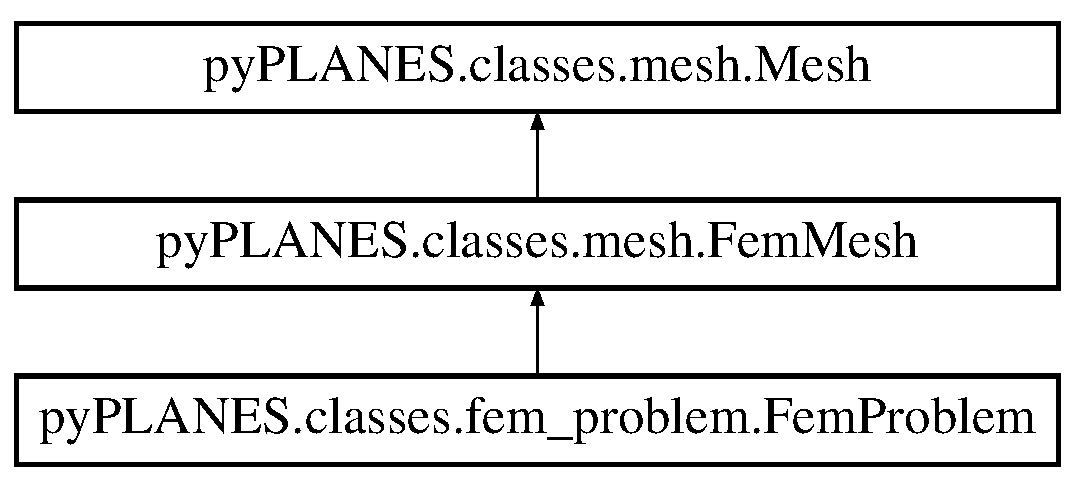
\includegraphics[height=3.000000cm]{classpy_p_l_a_n_e_s_1_1classes_1_1mesh_1_1_fem_mesh}
\end{center}
\end{figure}
\subsection*{Public Member Functions}
\begin{DoxyCompactItemize}
\item 
\mbox{\Hypertarget{classpy_p_l_a_n_e_s_1_1classes_1_1mesh_1_1_fem_mesh_a8407a55e891bad2d7cd06ddefe2c8963}\label{classpy_p_l_a_n_e_s_1_1classes_1_1mesh_1_1_fem_mesh_a8407a55e891bad2d7cd06ddefe2c8963}} 
def {\bfseries \+\_\+\+\_\+init\+\_\+\+\_\+} (self, kwargs)
\end{DoxyCompactItemize}
\subsection*{Additional Inherited Members}


The documentation for this class was generated from the following file\+:\begin{DoxyCompactItemize}
\item 
py\+P\+L\+A\+N\+E\+S/classes/mesh.\+py\end{DoxyCompactItemize}

\hypertarget{classpy_p_l_a_n_e_s_1_1classes_1_1fem__model_1_1_fem_model}{}\section{py\+P\+L\+A\+N\+E\+S.\+classes.\+fem\+\_\+model.\+Fem\+Model Class Reference}
\label{classpy_p_l_a_n_e_s_1_1classes_1_1fem__model_1_1_fem_model}\index{py\+P\+L\+A\+N\+E\+S.\+classes.\+fem\+\_\+model.\+Fem\+Model@{py\+P\+L\+A\+N\+E\+S.\+classes.\+fem\+\_\+model.\+Fem\+Model}}
Inheritance diagram for py\+P\+L\+A\+N\+E\+S.\+classes.\+fem\+\_\+model.\+Fem\+Model\+:\begin{figure}[H]
\begin{center}
\leavevmode
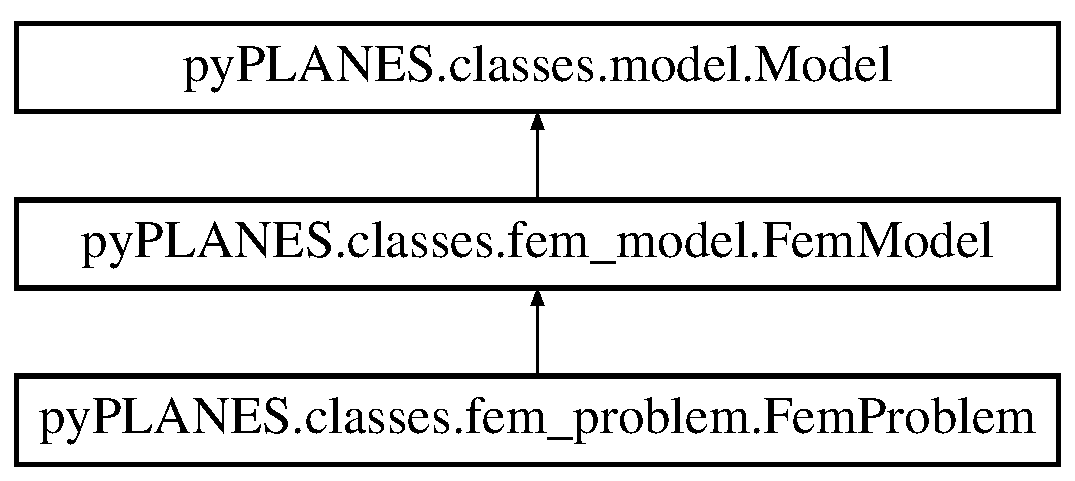
\includegraphics[height=3.000000cm]{classpy_p_l_a_n_e_s_1_1classes_1_1fem__model_1_1_fem_model}
\end{center}
\end{figure}
\subsection*{Public Member Functions}
\begin{DoxyCompactItemize}
\item 
\mbox{\Hypertarget{classpy_p_l_a_n_e_s_1_1classes_1_1fem__model_1_1_fem_model_a3e0cc597a3ba8070aa317ebc4d02a982}\label{classpy_p_l_a_n_e_s_1_1classes_1_1fem__model_1_1_fem_model_a3e0cc597a3ba8070aa317ebc4d02a982}} 
def {\bfseries \+\_\+\+\_\+init\+\_\+\+\_\+} (self, kwargs)
\item 
\mbox{\Hypertarget{classpy_p_l_a_n_e_s_1_1classes_1_1fem__model_1_1_fem_model_ab5d7bc2528d75574fe9a12518d5613f9}\label{classpy_p_l_a_n_e_s_1_1classes_1_1fem__model_1_1_fem_model_ab5d7bc2528d75574fe9a12518d5613f9}} 
def {\bfseries initialisation\+\_\+out\+\_\+files} (self)
\item 
\mbox{\Hypertarget{classpy_p_l_a_n_e_s_1_1classes_1_1fem__model_1_1_fem_model_af841f4640dfdd90c19b04c3f25b5842e}\label{classpy_p_l_a_n_e_s_1_1classes_1_1fem__model_1_1_fem_model_af841f4640dfdd90c19b04c3f25b5842e}} 
def {\bfseries write\+\_\+out\+\_\+files} (self)
\item 
\mbox{\Hypertarget{classpy_p_l_a_n_e_s_1_1classes_1_1fem__model_1_1_fem_model_ac3273f9f7157f21e6cf8b6efc6e25fb4}\label{classpy_p_l_a_n_e_s_1_1classes_1_1fem__model_1_1_fem_model_ac3273f9f7157f21e6cf8b6efc6e25fb4}} 
def {\bfseries \+\_\+\+\_\+str\+\_\+\+\_\+} (self)
\item 
\mbox{\Hypertarget{classpy_p_l_a_n_e_s_1_1classes_1_1fem__model_1_1_fem_model_a5b8c6ffb7d940989355a6712d8107a8a}\label{classpy_p_l_a_n_e_s_1_1classes_1_1fem__model_1_1_fem_model_a5b8c6ffb7d940989355a6712d8107a8a}} 
def {\bfseries resolution} (self)
\item 
\mbox{\Hypertarget{classpy_p_l_a_n_e_s_1_1classes_1_1fem__model_1_1_fem_model_aaf290478bbb34b7a4cd2a7e374ea4c29}\label{classpy_p_l_a_n_e_s_1_1classes_1_1fem__model_1_1_fem_model_aaf290478bbb34b7a4cd2a7e374ea4c29}} 
def {\bfseries linear\+\_\+system\+\_\+2\+\_\+numpy} (self)
\item 
\mbox{\Hypertarget{classpy_p_l_a_n_e_s_1_1classes_1_1fem__model_1_1_fem_model_af728ec30ed4908d6a3963395f022a915}\label{classpy_p_l_a_n_e_s_1_1classes_1_1fem__model_1_1_fem_model_af728ec30ed4908d6a3963395f022a915}} 
def {\bfseries create\+\_\+linear\+\_\+system} (self, f)
\item 
\mbox{\Hypertarget{classpy_p_l_a_n_e_s_1_1classes_1_1fem__model_1_1_fem_model_a9ca48e3b40a5b77e818092069c9d3fcd}\label{classpy_p_l_a_n_e_s_1_1classes_1_1fem__model_1_1_fem_model_a9ca48e3b40a5b77e818092069c9d3fcd}} 
def {\bfseries apply\+\_\+periodicity} (self)
\item 
\mbox{\Hypertarget{classpy_p_l_a_n_e_s_1_1classes_1_1fem__model_1_1_fem_model_a82abd36cfdd321e5d0e51a882f1ab788}\label{classpy_p_l_a_n_e_s_1_1classes_1_1fem__model_1_1_fem_model_a82abd36cfdd321e5d0e51a882f1ab788}} 
def {\bfseries solve} (self)
\end{DoxyCompactItemize}
\subsection*{Public Attributes}
\begin{DoxyCompactItemize}
\item 
\mbox{\Hypertarget{classpy_p_l_a_n_e_s_1_1classes_1_1fem__model_1_1_fem_model_a2928d12c3c33b1ee869f0ffe894d3f04}\label{classpy_p_l_a_n_e_s_1_1classes_1_1fem__model_1_1_fem_model_a2928d12c3c33b1ee869f0ffe894d3f04}} 
{\bfseries incident\+\_\+ml}
\item 
\mbox{\Hypertarget{classpy_p_l_a_n_e_s_1_1classes_1_1fem__model_1_1_fem_model_afa81f01f3baa1b7ca95a936c0d5b31a5}\label{classpy_p_l_a_n_e_s_1_1classes_1_1fem__model_1_1_fem_model_afa81f01f3baa1b7ca95a936c0d5b31a5}} 
{\bfseries reference\+\_\+elements}
\item 
\mbox{\Hypertarget{classpy_p_l_a_n_e_s_1_1classes_1_1fem__model_1_1_fem_model_a1a3584cf4dcb65b95e5d6320d25607de}\label{classpy_p_l_a_n_e_s_1_1classes_1_1fem__model_1_1_fem_model_a1a3584cf4dcb65b95e5d6320d25607de}} 
{\bfseries edges}
\item 
\mbox{\Hypertarget{classpy_p_l_a_n_e_s_1_1classes_1_1fem__model_1_1_fem_model_a269b60b9f8b17228f0acea5986a8ee90}\label{classpy_p_l_a_n_e_s_1_1classes_1_1fem__model_1_1_fem_model_a269b60b9f8b17228f0acea5986a8ee90}} 
{\bfseries faces}
\item 
\mbox{\Hypertarget{classpy_p_l_a_n_e_s_1_1classes_1_1fem__model_1_1_fem_model_aa3bc02b3ba22f3aa324ddc56e2a8a595}\label{classpy_p_l_a_n_e_s_1_1classes_1_1fem__model_1_1_fem_model_aa3bc02b3ba22f3aa324ddc56e2a8a595}} 
{\bfseries bubbles}
\item 
\mbox{\Hypertarget{classpy_p_l_a_n_e_s_1_1classes_1_1fem__model_1_1_fem_model_af674bef7ead2f9b1d60ef821bbc429df}\label{classpy_p_l_a_n_e_s_1_1classes_1_1fem__model_1_1_fem_model_af674bef7ead2f9b1d60ef821bbc429df}} 
{\bfseries nb\+\_\+edges}
\item 
\mbox{\Hypertarget{classpy_p_l_a_n_e_s_1_1classes_1_1fem__model_1_1_fem_model_a028fb7413a5f3dfc67454358ff482a5a}\label{classpy_p_l_a_n_e_s_1_1classes_1_1fem__model_1_1_fem_model_a028fb7413a5f3dfc67454358ff482a5a}} 
{\bfseries nb\+\_\+faces}
\item 
\mbox{\Hypertarget{classpy_p_l_a_n_e_s_1_1classes_1_1fem__model_1_1_fem_model_ad1830cd531b6d396ee415ffa84b20bce}\label{classpy_p_l_a_n_e_s_1_1classes_1_1fem__model_1_1_fem_model_ad1830cd531b6d396ee415ffa84b20bce}} 
{\bfseries nb\+\_\+bubbles}
\item 
\mbox{\Hypertarget{classpy_p_l_a_n_e_s_1_1classes_1_1fem__model_1_1_fem_model_adeb7ec61d5f4216c56738d8ebada5899}\label{classpy_p_l_a_n_e_s_1_1classes_1_1fem__model_1_1_fem_model_adeb7ec61d5f4216c56738d8ebada5899}} 
{\bfseries name\+\_\+server}
\item 
\mbox{\Hypertarget{classpy_p_l_a_n_e_s_1_1classes_1_1fem__model_1_1_fem_model_a9663adc66b8f32524ab16afa5426cf69}\label{classpy_p_l_a_n_e_s_1_1classes_1_1fem__model_1_1_fem_model_a9663adc66b8f32524ab16afa5426cf69}} 
{\bfseries F}
\item 
\mbox{\Hypertarget{classpy_p_l_a_n_e_s_1_1classes_1_1fem__model_1_1_fem_model_ab878778e7ebef753e68756ecf78e5e7a}\label{classpy_p_l_a_n_e_s_1_1classes_1_1fem__model_1_1_fem_model_ab878778e7ebef753e68756ecf78e5e7a}} 
{\bfseries A\+\_\+v}
\item 
\mbox{\Hypertarget{classpy_p_l_a_n_e_s_1_1classes_1_1fem__model_1_1_fem_model_aa2749aef1b582418b8a381fa63ec7d71}\label{classpy_p_l_a_n_e_s_1_1classes_1_1fem__model_1_1_fem_model_aa2749aef1b582418b8a381fa63ec7d71}} 
{\bfseries T\+\_\+v}
\item 
\mbox{\Hypertarget{classpy_p_l_a_n_e_s_1_1classes_1_1fem__model_1_1_fem_model_a523f5749fa01dc36948f5d5e63c2af98}\label{classpy_p_l_a_n_e_s_1_1classes_1_1fem__model_1_1_fem_model_a523f5749fa01dc36948f5d5e63c2af98}} 
{\bfseries A\+\_\+j\+\_\+c}
\item 
\mbox{\Hypertarget{classpy_p_l_a_n_e_s_1_1classes_1_1fem__model_1_1_fem_model_acb29f85ed1fcdf2dffdbe39c13e394b5}\label{classpy_p_l_a_n_e_s_1_1classes_1_1fem__model_1_1_fem_model_acb29f85ed1fcdf2dffdbe39c13e394b5}} 
{\bfseries A\+\_\+i}
\item 
\mbox{\Hypertarget{classpy_p_l_a_n_e_s_1_1classes_1_1fem__model_1_1_fem_model_a5980b34f53769bb0019ebc1d9d9c260b}\label{classpy_p_l_a_n_e_s_1_1classes_1_1fem__model_1_1_fem_model_a5980b34f53769bb0019ebc1d9d9c260b}} 
{\bfseries F\+\_\+i}
\item 
\mbox{\Hypertarget{classpy_p_l_a_n_e_s_1_1classes_1_1fem__model_1_1_fem_model_a3473e026f1571eff00f5d1738fea2e77}\label{classpy_p_l_a_n_e_s_1_1classes_1_1fem__model_1_1_fem_model_a3473e026f1571eff00f5d1738fea2e77}} 
{\bfseries A\+\_\+j}
\item 
\mbox{\Hypertarget{classpy_p_l_a_n_e_s_1_1classes_1_1fem__model_1_1_fem_model_aa29ef71833a1be9b81191a20e899ef75}\label{classpy_p_l_a_n_e_s_1_1classes_1_1fem__model_1_1_fem_model_aa29ef71833a1be9b81191a20e899ef75}} 
{\bfseries nb\+\_\+dof\+\_\+condensed}
\item 
\mbox{\Hypertarget{classpy_p_l_a_n_e_s_1_1classes_1_1fem__model_1_1_fem_model_a4489bcd02595507f0a10e3162051f43f}\label{classpy_p_l_a_n_e_s_1_1classes_1_1fem__model_1_1_fem_model_a4489bcd02595507f0a10e3162051f43f}} 
{\bfseries F\+\_\+v}
\item 
\mbox{\Hypertarget{classpy_p_l_a_n_e_s_1_1classes_1_1fem__model_1_1_fem_model_a1ddf343343b66acf18e7b9a03ece9dcd}\label{classpy_p_l_a_n_e_s_1_1classes_1_1fem__model_1_1_fem_model_a1ddf343343b66acf18e7b9a03ece9dcd}} 
{\bfseries modulus\+\_\+reflex}
\item 
\mbox{\Hypertarget{classpy_p_l_a_n_e_s_1_1classes_1_1fem__model_1_1_fem_model_a245f534453513881cd07e617f02603af}\label{classpy_p_l_a_n_e_s_1_1classes_1_1fem__model_1_1_fem_model_a245f534453513881cd07e617f02603af}} 
{\bfseries modulus\+\_\+trans}
\end{DoxyCompactItemize}


The documentation for this class was generated from the following file\+:\begin{DoxyCompactItemize}
\item 
py\+P\+L\+A\+N\+E\+S/classes/fem\+\_\+model.\+py\end{DoxyCompactItemize}

\hypertarget{classpy_p_l_a_n_e_s_1_1classes_1_1fem__problem_1_1_fem_problem}{}\section{py\+P\+L\+A\+N\+E\+S.\+classes.\+fem\+\_\+problem.\+Fem\+Problem Class Reference}
\label{classpy_p_l_a_n_e_s_1_1classes_1_1fem__problem_1_1_fem_problem}\index{py\+P\+L\+A\+N\+E\+S.\+classes.\+fem\+\_\+problem.\+Fem\+Problem@{py\+P\+L\+A\+N\+E\+S.\+classes.\+fem\+\_\+problem.\+Fem\+Problem}}
Inheritance diagram for py\+P\+L\+A\+N\+E\+S.\+classes.\+fem\+\_\+problem.\+Fem\+Problem\+:\begin{figure}[H]
\begin{center}
\leavevmode
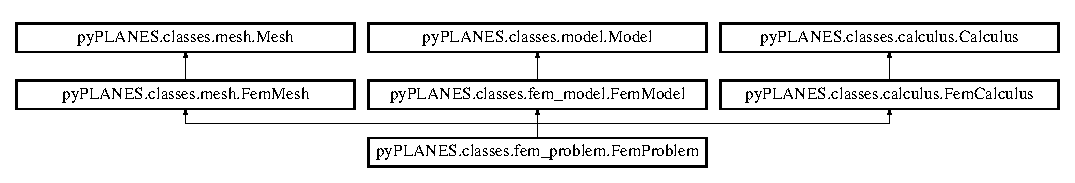
\includegraphics[height=2.007169cm]{classpy_p_l_a_n_e_s_1_1classes_1_1fem__problem_1_1_fem_problem}
\end{center}
\end{figure}
\subsection*{Public Member Functions}
\begin{DoxyCompactItemize}
\item 
\mbox{\Hypertarget{classpy_p_l_a_n_e_s_1_1classes_1_1fem__problem_1_1_fem_problem_a95c28bb0f21dd60d3df0196bff6a09ed}\label{classpy_p_l_a_n_e_s_1_1classes_1_1fem__problem_1_1_fem_problem_a95c28bb0f21dd60d3df0196bff6a09ed}} 
def {\bfseries \+\_\+\+\_\+init\+\_\+\+\_\+} (self, kwargs)
\item 
\mbox{\Hypertarget{classpy_p_l_a_n_e_s_1_1classes_1_1fem__problem_1_1_fem_problem_aa27a7d9c65a5e6e7b86ca6aade2342ef}\label{classpy_p_l_a_n_e_s_1_1classes_1_1fem__problem_1_1_fem_problem_aa27a7d9c65a5e6e7b86ca6aade2342ef}} 
def {\bfseries resolution} (self)
\end{DoxyCompactItemize}
\subsection*{Public Attributes}
\begin{DoxyCompactItemize}
\item 
\mbox{\Hypertarget{classpy_p_l_a_n_e_s_1_1classes_1_1fem__problem_1_1_fem_problem_aafceee4e18cf0f7a7e6422ad4687b262}\label{classpy_p_l_a_n_e_s_1_1classes_1_1fem__problem_1_1_fem_problem_aafceee4e18cf0f7a7e6422ad4687b262}} 
{\bfseries name\+\_\+server}
\item 
\mbox{\Hypertarget{classpy_p_l_a_n_e_s_1_1classes_1_1fem__problem_1_1_fem_problem_acda71a21344dd0f1250d0ca0a6bd54a6}\label{classpy_p_l_a_n_e_s_1_1classes_1_1fem__problem_1_1_fem_problem_acda71a21344dd0f1250d0ca0a6bd54a6}} 
{\bfseries verbose}
\item 
\mbox{\Hypertarget{classpy_p_l_a_n_e_s_1_1classes_1_1fem__problem_1_1_fem_problem_aeda1dac1f03f6ace5d02349698fecdb3}\label{classpy_p_l_a_n_e_s_1_1classes_1_1fem__problem_1_1_fem_problem_aeda1dac1f03f6ace5d02349698fecdb3}} 
{\bfseries order}
\item 
\mbox{\Hypertarget{classpy_p_l_a_n_e_s_1_1classes_1_1fem__problem_1_1_fem_problem_a5616b175344610a5f49cab753f47f414}\label{classpy_p_l_a_n_e_s_1_1classes_1_1fem__problem_1_1_fem_problem_a5616b175344610a5f49cab753f47f414}} 
{\bfseries interface\+\_\+zone}
\item 
\mbox{\Hypertarget{classpy_p_l_a_n_e_s_1_1classes_1_1fem__problem_1_1_fem_problem_acaf6839babe57657f539ac5596888731}\label{classpy_p_l_a_n_e_s_1_1classes_1_1fem__problem_1_1_fem_problem_acaf6839babe57657f539ac5596888731}} 
{\bfseries dim}
\item 
\mbox{\Hypertarget{classpy_p_l_a_n_e_s_1_1classes_1_1fem__problem_1_1_fem_problem_a7294ee34c7295bba1ef619bcf181897f}\label{classpy_p_l_a_n_e_s_1_1classes_1_1fem__problem_1_1_fem_problem_a7294ee34c7295bba1ef619bcf181897f}} 
{\bfseries duration\+\_\+importation}
\item 
\mbox{\Hypertarget{classpy_p_l_a_n_e_s_1_1classes_1_1fem__problem_1_1_fem_problem_a7d0400451677296cc8cf720461188f7f}\label{classpy_p_l_a_n_e_s_1_1classes_1_1fem__problem_1_1_fem_problem_a7d0400451677296cc8cf720461188f7f}} 
{\bfseries duration\+\_\+assembly}
\end{DoxyCompactItemize}


The documentation for this class was generated from the following file\+:\begin{DoxyCompactItemize}
\item 
py\+P\+L\+A\+N\+E\+S/classes/fem\+\_\+problem.\+py\end{DoxyCompactItemize}

\hypertarget{classpy_p_l_a_n_e_s_1_1classes_1_1entity__classes_1_1_fluid_fem}{}\section{py\+P\+L\+A\+N\+E\+S.\+classes.\+entity\+\_\+classes.\+Fluid\+Fem Class Reference}
\label{classpy_p_l_a_n_e_s_1_1classes_1_1entity__classes_1_1_fluid_fem}\index{py\+P\+L\+A\+N\+E\+S.\+classes.\+entity\+\_\+classes.\+Fluid\+Fem@{py\+P\+L\+A\+N\+E\+S.\+classes.\+entity\+\_\+classes.\+Fluid\+Fem}}
Inheritance diagram for py\+P\+L\+A\+N\+E\+S.\+classes.\+entity\+\_\+classes.\+Fluid\+Fem\+:\begin{figure}[H]
\begin{center}
\leavevmode
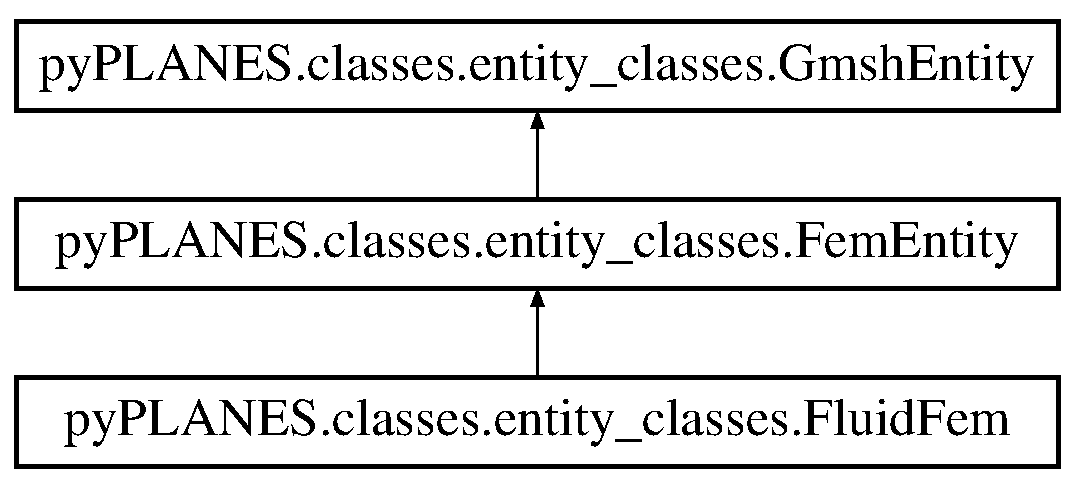
\includegraphics[height=3.000000cm]{classpy_p_l_a_n_e_s_1_1classes_1_1entity__classes_1_1_fluid_fem}
\end{center}
\end{figure}
\subsection*{Public Member Functions}
\begin{DoxyCompactItemize}
\item 
\mbox{\Hypertarget{classpy_p_l_a_n_e_s_1_1classes_1_1entity__classes_1_1_fluid_fem_a719ab79825fef3cff63deb22f46be94f}\label{classpy_p_l_a_n_e_s_1_1classes_1_1entity__classes_1_1_fluid_fem_a719ab79825fef3cff63deb22f46be94f}} 
def {\bfseries \+\_\+\+\_\+init\+\_\+\+\_\+} (self, kwargs)
\item 
\mbox{\Hypertarget{classpy_p_l_a_n_e_s_1_1classes_1_1entity__classes_1_1_fluid_fem_af7fdbd6e5fbfbe6f04e105338dbdf8ed}\label{classpy_p_l_a_n_e_s_1_1classes_1_1entity__classes_1_1_fluid_fem_af7fdbd6e5fbfbe6f04e105338dbdf8ed}} 
def {\bfseries \+\_\+\+\_\+str\+\_\+\+\_\+} (self)
\item 
\mbox{\Hypertarget{classpy_p_l_a_n_e_s_1_1classes_1_1entity__classes_1_1_fluid_fem_a1bee421000201f512ba1718afef7dc6d}\label{classpy_p_l_a_n_e_s_1_1classes_1_1entity__classes_1_1_fluid_fem_a1bee421000201f512ba1718afef7dc6d}} 
def {\bfseries elementary\+\_\+matrices} (self, \+\_\+el)
\item 
\mbox{\Hypertarget{classpy_p_l_a_n_e_s_1_1classes_1_1entity__classes_1_1_fluid_fem_acf1f23520a698cf1b5586ec49ae18e21}\label{classpy_p_l_a_n_e_s_1_1classes_1_1entity__classes_1_1_fluid_fem_acf1f23520a698cf1b5586ec49ae18e21}} 
def {\bfseries append\+\_\+linear\+\_\+system} (self, omega)
\end{DoxyCompactItemize}
\subsection*{Public Attributes}
\begin{DoxyCompactItemize}
\item 
\mbox{\Hypertarget{classpy_p_l_a_n_e_s_1_1classes_1_1entity__classes_1_1_fluid_fem_aa12deb6c05820332adad7509067c14cc}\label{classpy_p_l_a_n_e_s_1_1classes_1_1entity__classes_1_1_fluid_fem_aa12deb6c05820332adad7509067c14cc}} 
{\bfseries mat}
\item 
\mbox{\Hypertarget{classpy_p_l_a_n_e_s_1_1classes_1_1entity__classes_1_1_fluid_fem_ac7f09f190b559f83968a4961037bdbdc}\label{classpy_p_l_a_n_e_s_1_1classes_1_1entity__classes_1_1_fluid_fem_ac7f09f190b559f83968a4961037bdbdc}} 
{\bfseries H\+\_\+v}
\item 
\mbox{\Hypertarget{classpy_p_l_a_n_e_s_1_1classes_1_1entity__classes_1_1_fluid_fem_af8cdfa08aa11586936f2ebe5e1f54193}\label{classpy_p_l_a_n_e_s_1_1classes_1_1entity__classes_1_1_fluid_fem_af8cdfa08aa11586936f2ebe5e1f54193}} 
{\bfseries Q\+\_\+v}
\end{DoxyCompactItemize}


The documentation for this class was generated from the following file\+:\begin{DoxyCompactItemize}
\item 
py\+P\+L\+A\+N\+E\+S/classes/entity\+\_\+classes.\+py\end{DoxyCompactItemize}

\hypertarget{classpy_p_l_a_n_e_s_1_1classes_1_1entity__classes_1_1_fluid_structure_fem}{}\section{py\+P\+L\+A\+N\+E\+S.\+classes.\+entity\+\_\+classes.\+Fluid\+Structure\+Fem Class Reference}
\label{classpy_p_l_a_n_e_s_1_1classes_1_1entity__classes_1_1_fluid_structure_fem}\index{py\+P\+L\+A\+N\+E\+S.\+classes.\+entity\+\_\+classes.\+Fluid\+Structure\+Fem@{py\+P\+L\+A\+N\+E\+S.\+classes.\+entity\+\_\+classes.\+Fluid\+Structure\+Fem}}
Inheritance diagram for py\+P\+L\+A\+N\+E\+S.\+classes.\+entity\+\_\+classes.\+Fluid\+Structure\+Fem\+:\begin{figure}[H]
\begin{center}
\leavevmode
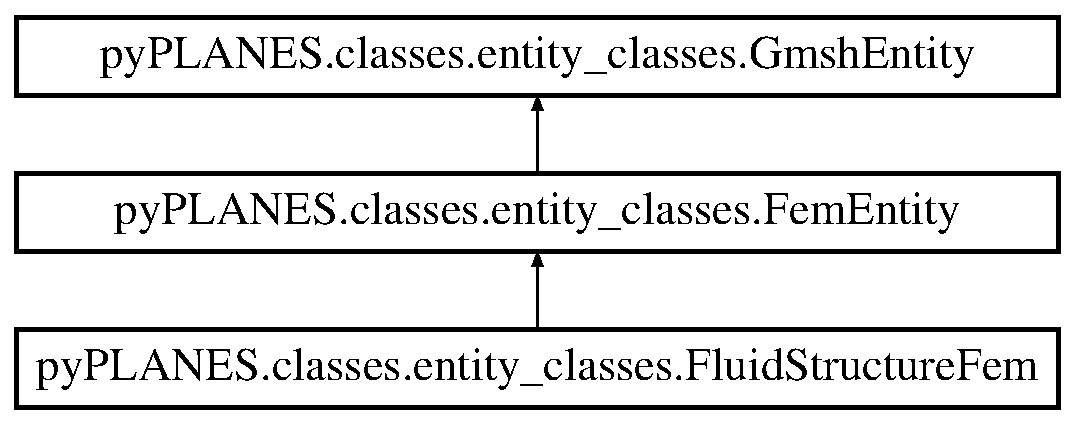
\includegraphics[height=3.000000cm]{classpy_p_l_a_n_e_s_1_1classes_1_1entity__classes_1_1_fluid_structure_fem}
\end{center}
\end{figure}
\subsection*{Public Member Functions}
\begin{DoxyCompactItemize}
\item 
\mbox{\Hypertarget{classpy_p_l_a_n_e_s_1_1classes_1_1entity__classes_1_1_fluid_structure_fem_acbe38b6ddf617a116355ca0b2c3f2ad4}\label{classpy_p_l_a_n_e_s_1_1classes_1_1entity__classes_1_1_fluid_structure_fem_acbe38b6ddf617a116355ca0b2c3f2ad4}} 
def {\bfseries \+\_\+\+\_\+init\+\_\+\+\_\+} (self, kwargs)
\item 
\mbox{\Hypertarget{classpy_p_l_a_n_e_s_1_1classes_1_1entity__classes_1_1_fluid_structure_fem_a257b04e97ca4699c69c8f3197d1c67ba}\label{classpy_p_l_a_n_e_s_1_1classes_1_1entity__classes_1_1_fluid_structure_fem_a257b04e97ca4699c69c8f3197d1c67ba}} 
def {\bfseries elementary\+\_\+matrices} (self, \+\_\+el)
\item 
\mbox{\Hypertarget{classpy_p_l_a_n_e_s_1_1classes_1_1entity__classes_1_1_fluid_structure_fem_ae44887442c22938a36ff724f7f32b040}\label{classpy_p_l_a_n_e_s_1_1classes_1_1entity__classes_1_1_fluid_structure_fem_ae44887442c22938a36ff724f7f32b040}} 
def {\bfseries \+\_\+\+\_\+str\+\_\+\+\_\+} (self)
\item 
\mbox{\Hypertarget{classpy_p_l_a_n_e_s_1_1classes_1_1entity__classes_1_1_fluid_structure_fem_a49ee0683cd8ba82c1bbfeded355ec9aa}\label{classpy_p_l_a_n_e_s_1_1classes_1_1entity__classes_1_1_fluid_structure_fem_a49ee0683cd8ba82c1bbfeded355ec9aa}} 
def {\bfseries append\+\_\+linear\+\_\+system} (self, omega)
\end{DoxyCompactItemize}
\subsection*{Public Attributes}
\begin{DoxyCompactItemize}
\item 
\mbox{\Hypertarget{classpy_p_l_a_n_e_s_1_1classes_1_1entity__classes_1_1_fluid_structure_fem_a815d55908cb15a9240b88d4a5a636a09}\label{classpy_p_l_a_n_e_s_1_1classes_1_1entity__classes_1_1_fluid_structure_fem_a815d55908cb15a9240b88d4a5a636a09}} 
{\bfseries fluid\+\_\+neighbour}
\item 
\mbox{\Hypertarget{classpy_p_l_a_n_e_s_1_1classes_1_1entity__classes_1_1_fluid_structure_fem_a0d967d9b060bedc6c46739ff3c0e3604}\label{classpy_p_l_a_n_e_s_1_1classes_1_1entity__classes_1_1_fluid_structure_fem_a0d967d9b060bedc6c46739ff3c0e3604}} 
{\bfseries struc\+\_\+neighbour}
\end{DoxyCompactItemize}


The documentation for this class was generated from the following file\+:\begin{DoxyCompactItemize}
\item 
py\+P\+L\+A\+N\+E\+S/classes/entity\+\_\+classes.\+py\end{DoxyCompactItemize}

\hypertarget{classpy_p_l_a_n_e_s_1_1gmsh_1_1write__geo__file_1_1_gmsh}{}\section{py\+P\+L\+A\+N\+E\+S.\+gmsh.\+write\+\_\+geo\+\_\+file.\+Gmsh Class Reference}
\label{classpy_p_l_a_n_e_s_1_1gmsh_1_1write__geo__file_1_1_gmsh}\index{py\+P\+L\+A\+N\+E\+S.\+gmsh.\+write\+\_\+geo\+\_\+file.\+Gmsh@{py\+P\+L\+A\+N\+E\+S.\+gmsh.\+write\+\_\+geo\+\_\+file.\+Gmsh}}
\subsection*{Classes}
\begin{DoxyCompactItemize}
\item 
class \mbox{\hyperlink{classpy_p_l_a_n_e_s_1_1gmsh_1_1write__geo__file_1_1_gmsh_1_1_circle}{Circle}}
\item 
class \mbox{\hyperlink{classpy_p_l_a_n_e_s_1_1gmsh_1_1write__geo__file_1_1_gmsh_1_1_line}{Line}}
\item 
class \mbox{\hyperlink{classpy_p_l_a_n_e_s_1_1gmsh_1_1write__geo__file_1_1_gmsh_1_1_line_loop}{Line\+Loop}}
\item 
class \mbox{\hyperlink{classpy_p_l_a_n_e_s_1_1gmsh_1_1write__geo__file_1_1_gmsh_1_1_point}{Point}}
\item 
class \mbox{\hyperlink{classpy_p_l_a_n_e_s_1_1gmsh_1_1write__geo__file_1_1_gmsh_1_1_surface}{Surface}}
\end{DoxyCompactItemize}
\subsection*{Public Member Functions}
\begin{DoxyCompactItemize}
\item 
\mbox{\Hypertarget{classpy_p_l_a_n_e_s_1_1gmsh_1_1write__geo__file_1_1_gmsh_a1423275017b0c62e1d88ec50350d2b90}\label{classpy_p_l_a_n_e_s_1_1gmsh_1_1write__geo__file_1_1_gmsh_a1423275017b0c62e1d88ec50350d2b90}} 
def {\bfseries \+\_\+\+\_\+init\+\_\+\+\_\+} (self, file=\char`\"{}noname\char`\"{})
\item 
\mbox{\Hypertarget{classpy_p_l_a_n_e_s_1_1gmsh_1_1write__geo__file_1_1_gmsh_ad5cb6e06ea90a83c8ae848040870a4a7}\label{classpy_p_l_a_n_e_s_1_1gmsh_1_1write__geo__file_1_1_gmsh_ad5cb6e06ea90a83c8ae848040870a4a7}} 
def {\bfseries add} (self, txt)
\item 
\mbox{\Hypertarget{classpy_p_l_a_n_e_s_1_1gmsh_1_1write__geo__file_1_1_gmsh_a790fd8b59f5d0875b05c85b472f67f6a}\label{classpy_p_l_a_n_e_s_1_1gmsh_1_1write__geo__file_1_1_gmsh_a790fd8b59f5d0875b05c85b472f67f6a}} 
def {\bfseries new\+\_\+point} (self, x, y, lc)
\item 
\mbox{\Hypertarget{classpy_p_l_a_n_e_s_1_1gmsh_1_1write__geo__file_1_1_gmsh_ac431ea22be48438a417b7c336fbe399b}\label{classpy_p_l_a_n_e_s_1_1gmsh_1_1write__geo__file_1_1_gmsh_ac431ea22be48438a417b7c336fbe399b}} 
def {\bfseries new\+\_\+line} (self, \+\_\+1, \+\_\+2)
\item 
\mbox{\Hypertarget{classpy_p_l_a_n_e_s_1_1gmsh_1_1write__geo__file_1_1_gmsh_a28685c85ec95814742172df2898d8d64}\label{classpy_p_l_a_n_e_s_1_1gmsh_1_1write__geo__file_1_1_gmsh_a28685c85ec95814742172df2898d8d64}} 
def {\bfseries new\+\_\+line\+\_\+loop} (self, \+\_\+list)
\item 
\mbox{\Hypertarget{classpy_p_l_a_n_e_s_1_1gmsh_1_1write__geo__file_1_1_gmsh_a283acef9df029ce0323727654afbaed8}\label{classpy_p_l_a_n_e_s_1_1gmsh_1_1write__geo__file_1_1_gmsh_a283acef9df029ce0323727654afbaed8}} 
def {\bfseries new\+\_\+surface} (self, ll)
\item 
\mbox{\Hypertarget{classpy_p_l_a_n_e_s_1_1gmsh_1_1write__geo__file_1_1_gmsh_a30a501696fa07899475caa5423fb492d}\label{classpy_p_l_a_n_e_s_1_1gmsh_1_1write__geo__file_1_1_gmsh_a30a501696fa07899475caa5423fb492d}} 
def {\bfseries new\+\_\+circle} (self, x\+\_\+0, y\+\_\+0, r, lc)
\item 
\mbox{\Hypertarget{classpy_p_l_a_n_e_s_1_1gmsh_1_1write__geo__file_1_1_gmsh_ae195750caceaca331ad7f9bd3c296a11}\label{classpy_p_l_a_n_e_s_1_1gmsh_1_1write__geo__file_1_1_gmsh_ae195750caceaca331ad7f9bd3c296a11}} 
def {\bfseries new\+\_\+physical} (self, obj, label)
\item 
\mbox{\Hypertarget{classpy_p_l_a_n_e_s_1_1gmsh_1_1write__geo__file_1_1_gmsh_aa56ef3e141e889154b21bd8e6c17196a}\label{classpy_p_l_a_n_e_s_1_1gmsh_1_1write__geo__file_1_1_gmsh_aa56ef3e141e889154b21bd8e6c17196a}} 
def {\bfseries new\+\_\+physical\+\_\+curve} (self, list, label)
\item 
\mbox{\Hypertarget{classpy_p_l_a_n_e_s_1_1gmsh_1_1write__geo__file_1_1_gmsh_ac551f383ba4c2738863db01968d3c3f4}\label{classpy_p_l_a_n_e_s_1_1gmsh_1_1write__geo__file_1_1_gmsh_ac551f383ba4c2738863db01968d3c3f4}} 
def {\bfseries new\+\_\+periodicity} (self, obj1, obj2, Delta)
\item 
\mbox{\Hypertarget{classpy_p_l_a_n_e_s_1_1gmsh_1_1write__geo__file_1_1_gmsh_a570d941b084f57370feb48a7d453cdf6}\label{classpy_p_l_a_n_e_s_1_1gmsh_1_1write__geo__file_1_1_gmsh_a570d941b084f57370feb48a7d453cdf6}} 
def {\bfseries run\+\_\+gmsh} (self, option=\char`\"{}\char`\"{})
\end{DoxyCompactItemize}
\subsection*{Public Attributes}
\begin{DoxyCompactItemize}
\item 
\mbox{\Hypertarget{classpy_p_l_a_n_e_s_1_1gmsh_1_1write__geo__file_1_1_gmsh_a5307f58569670ccdcd38fc31e2e20f17}\label{classpy_p_l_a_n_e_s_1_1gmsh_1_1write__geo__file_1_1_gmsh_a5307f58569670ccdcd38fc31e2e20f17}} 
{\bfseries geo\+\_\+file}
\item 
\mbox{\Hypertarget{classpy_p_l_a_n_e_s_1_1gmsh_1_1write__geo__file_1_1_gmsh_a689a51624ed9ea72c48c712d84ca061e}\label{classpy_p_l_a_n_e_s_1_1gmsh_1_1write__geo__file_1_1_gmsh_a689a51624ed9ea72c48c712d84ca061e}} 
{\bfseries f}
\item 
\mbox{\Hypertarget{classpy_p_l_a_n_e_s_1_1gmsh_1_1write__geo__file_1_1_gmsh_a306aaab890611d1b8ea5e4feee56110a}\label{classpy_p_l_a_n_e_s_1_1gmsh_1_1write__geo__file_1_1_gmsh_a306aaab890611d1b8ea5e4feee56110a}} 
{\bfseries nb\+\_\+tags}
\end{DoxyCompactItemize}


The documentation for this class was generated from the following file\+:\begin{DoxyCompactItemize}
\item 
py\+P\+L\+A\+N\+E\+S/gmsh/write\+\_\+geo\+\_\+file.\+py\end{DoxyCompactItemize}

\hypertarget{classpy_p_l_a_n_e_s_1_1classes_1_1entity__classes_1_1_gmsh_entity}{}\section{py\+P\+L\+A\+N\+E\+S.\+classes.\+entity\+\_\+classes.\+Gmsh\+Entity Class Reference}
\label{classpy_p_l_a_n_e_s_1_1classes_1_1entity__classes_1_1_gmsh_entity}\index{py\+P\+L\+A\+N\+E\+S.\+classes.\+entity\+\_\+classes.\+Gmsh\+Entity@{py\+P\+L\+A\+N\+E\+S.\+classes.\+entity\+\_\+classes.\+Gmsh\+Entity}}
Inheritance diagram for py\+P\+L\+A\+N\+E\+S.\+classes.\+entity\+\_\+classes.\+Gmsh\+Entity\+:\begin{figure}[H]
\begin{center}
\leavevmode
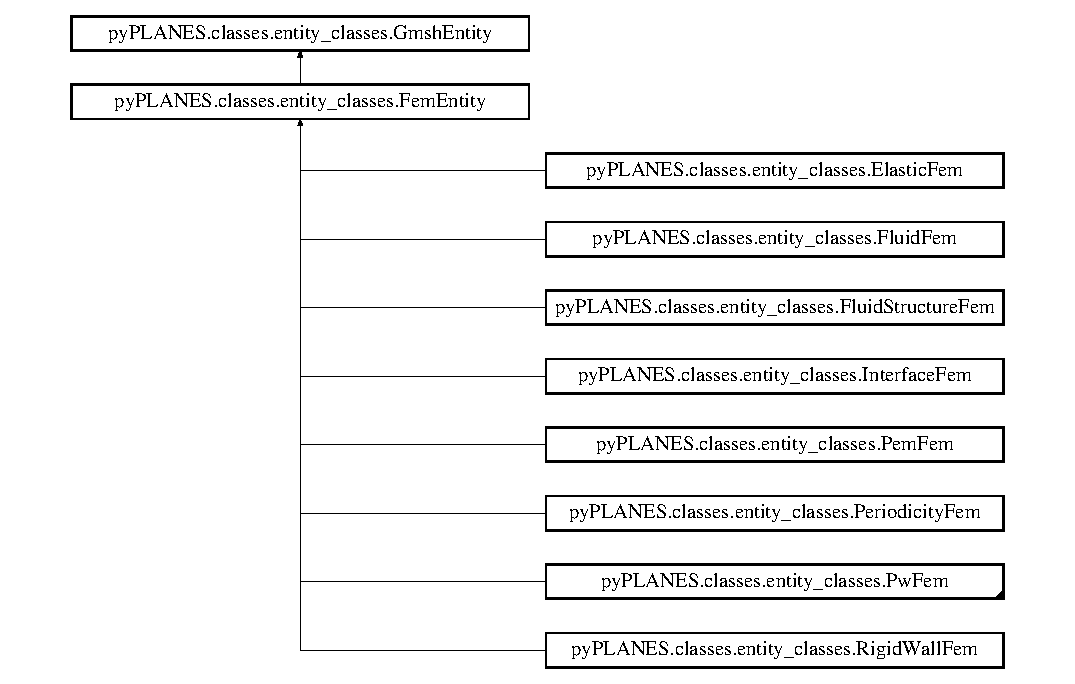
\includegraphics[height=8.750000cm]{classpy_p_l_a_n_e_s_1_1classes_1_1entity__classes_1_1_gmsh_entity}
\end{center}
\end{figure}
\subsection*{Public Member Functions}
\begin{DoxyCompactItemize}
\item 
\mbox{\Hypertarget{classpy_p_l_a_n_e_s_1_1classes_1_1entity__classes_1_1_gmsh_entity_ac0b16634fcb368904b7d9a7cb1475238}\label{classpy_p_l_a_n_e_s_1_1classes_1_1entity__classes_1_1_gmsh_entity_ac0b16634fcb368904b7d9a7cb1475238}} 
def {\bfseries \+\_\+\+\_\+init\+\_\+\+\_\+} (self, kwargs)
\item 
\mbox{\Hypertarget{classpy_p_l_a_n_e_s_1_1classes_1_1entity__classes_1_1_gmsh_entity_acdad5ba14e121280df533bdb3da862d5}\label{classpy_p_l_a_n_e_s_1_1classes_1_1entity__classes_1_1_gmsh_entity_acdad5ba14e121280df533bdb3da862d5}} 
def {\bfseries \+\_\+\+\_\+str\+\_\+\+\_\+} (self)
\end{DoxyCompactItemize}
\subsection*{Public Attributes}
\begin{DoxyCompactItemize}
\item 
\mbox{\Hypertarget{classpy_p_l_a_n_e_s_1_1classes_1_1entity__classes_1_1_gmsh_entity_aba65e02fd0f47e5a573335bf1e0670e5}\label{classpy_p_l_a_n_e_s_1_1classes_1_1entity__classes_1_1_gmsh_entity_aba65e02fd0f47e5a573335bf1e0670e5}} 
{\bfseries dim}
\item 
\mbox{\Hypertarget{classpy_p_l_a_n_e_s_1_1classes_1_1entity__classes_1_1_gmsh_entity_a03816c1306d58d0f0eca862cf6b0193b}\label{classpy_p_l_a_n_e_s_1_1classes_1_1entity__classes_1_1_gmsh_entity_a03816c1306d58d0f0eca862cf6b0193b}} 
{\bfseries tag}
\item 
\mbox{\Hypertarget{classpy_p_l_a_n_e_s_1_1classes_1_1entity__classes_1_1_gmsh_entity_a1557d0dd15506ae8f131e485968d7fe5}\label{classpy_p_l_a_n_e_s_1_1classes_1_1entity__classes_1_1_gmsh_entity_a1557d0dd15506ae8f131e485968d7fe5}} 
{\bfseries physical\+\_\+tags}
\item 
\mbox{\Hypertarget{classpy_p_l_a_n_e_s_1_1classes_1_1entity__classes_1_1_gmsh_entity_a4f1c1e5833f353e60fb0af9329fdad11}\label{classpy_p_l_a_n_e_s_1_1classes_1_1entity__classes_1_1_gmsh_entity_a4f1c1e5833f353e60fb0af9329fdad11}} 
{\bfseries neighbouring\+\_\+curves}
\item 
\mbox{\Hypertarget{classpy_p_l_a_n_e_s_1_1classes_1_1entity__classes_1_1_gmsh_entity_a66e4bb58145b12ca3463965ade63ca22}\label{classpy_p_l_a_n_e_s_1_1classes_1_1entity__classes_1_1_gmsh_entity_a66e4bb58145b12ca3463965ade63ca22}} 
{\bfseries x}
\item 
\mbox{\Hypertarget{classpy_p_l_a_n_e_s_1_1classes_1_1entity__classes_1_1_gmsh_entity_a549dbdfe4c22692b55562ad1e08199be}\label{classpy_p_l_a_n_e_s_1_1classes_1_1entity__classes_1_1_gmsh_entity_a549dbdfe4c22692b55562ad1e08199be}} 
{\bfseries y}
\item 
\mbox{\Hypertarget{classpy_p_l_a_n_e_s_1_1classes_1_1entity__classes_1_1_gmsh_entity_a0e49cfdab39497a91de459db16496d49}\label{classpy_p_l_a_n_e_s_1_1classes_1_1entity__classes_1_1_gmsh_entity_a0e49cfdab39497a91de459db16496d49}} 
{\bfseries z}
\item 
\mbox{\Hypertarget{classpy_p_l_a_n_e_s_1_1classes_1_1entity__classes_1_1_gmsh_entity_a9189e609a45b6419e82b033b8dd19ae1}\label{classpy_p_l_a_n_e_s_1_1classes_1_1entity__classes_1_1_gmsh_entity_a9189e609a45b6419e82b033b8dd19ae1}} 
{\bfseries coord}
\item 
\mbox{\Hypertarget{classpy_p_l_a_n_e_s_1_1classes_1_1entity__classes_1_1_gmsh_entity_a625145d010d1afa6fd2882abbee81f0b}\label{classpy_p_l_a_n_e_s_1_1classes_1_1entity__classes_1_1_gmsh_entity_a625145d010d1afa6fd2882abbee81f0b}} 
{\bfseries neighbours}
\item 
\mbox{\Hypertarget{classpy_p_l_a_n_e_s_1_1classes_1_1entity__classes_1_1_gmsh_entity_a56bf1430c0a027ef0b4972ef767dce26}\label{classpy_p_l_a_n_e_s_1_1classes_1_1entity__classes_1_1_gmsh_entity_a56bf1430c0a027ef0b4972ef767dce26}} 
{\bfseries neighbouring\+\_\+surfaces}
\item 
\mbox{\Hypertarget{classpy_p_l_a_n_e_s_1_1classes_1_1entity__classes_1_1_gmsh_entity_a311fc68c956375ff96c16c0ad9c3d577}\label{classpy_p_l_a_n_e_s_1_1classes_1_1entity__classes_1_1_gmsh_entity_a311fc68c956375ff96c16c0ad9c3d577}} 
{\bfseries bounding\+\_\+points}
\item 
\mbox{\Hypertarget{classpy_p_l_a_n_e_s_1_1classes_1_1entity__classes_1_1_gmsh_entity_a17baa477d344b3d4a43d438f5ad198ec}\label{classpy_p_l_a_n_e_s_1_1classes_1_1entity__classes_1_1_gmsh_entity_a17baa477d344b3d4a43d438f5ad198ec}} 
{\bfseries center}
\item 
\mbox{\Hypertarget{classpy_p_l_a_n_e_s_1_1classes_1_1entity__classes_1_1_gmsh_entity_a970fca248dddd6f56d0eb466483cb633}\label{classpy_p_l_a_n_e_s_1_1classes_1_1entity__classes_1_1_gmsh_entity_a970fca248dddd6f56d0eb466483cb633}} 
{\bfseries bounding\+\_\+curves}
\end{DoxyCompactItemize}


The documentation for this class was generated from the following file\+:\begin{DoxyCompactItemize}
\item 
py\+P\+L\+A\+N\+E\+S/classes/entity\+\_\+classes.\+py\end{DoxyCompactItemize}

\hypertarget{classpy_p_l_a_n_e_s_1_1classes_1_1entity__classes_1_1_incident_pw_fem}{}\section{py\+P\+L\+A\+N\+E\+S.\+classes.\+entity\+\_\+classes.\+Incident\+Pw\+Fem Class Reference}
\label{classpy_p_l_a_n_e_s_1_1classes_1_1entity__classes_1_1_incident_pw_fem}\index{py\+P\+L\+A\+N\+E\+S.\+classes.\+entity\+\_\+classes.\+Incident\+Pw\+Fem@{py\+P\+L\+A\+N\+E\+S.\+classes.\+entity\+\_\+classes.\+Incident\+Pw\+Fem}}
Inheritance diagram for py\+P\+L\+A\+N\+E\+S.\+classes.\+entity\+\_\+classes.\+Incident\+Pw\+Fem\+:\begin{figure}[H]
\begin{center}
\leavevmode
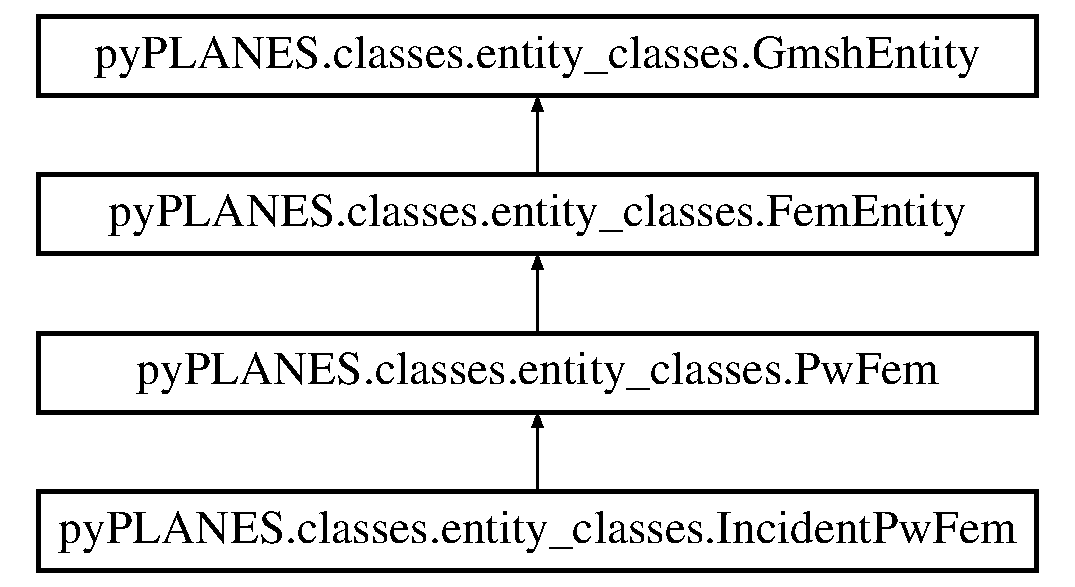
\includegraphics[height=4.000000cm]{classpy_p_l_a_n_e_s_1_1classes_1_1entity__classes_1_1_incident_pw_fem}
\end{center}
\end{figure}
\subsection*{Public Member Functions}
\begin{DoxyCompactItemize}
\item 
\mbox{\Hypertarget{classpy_p_l_a_n_e_s_1_1classes_1_1entity__classes_1_1_incident_pw_fem_aedc757aa9d62a8d5c7b651c97e0b990f}\label{classpy_p_l_a_n_e_s_1_1classes_1_1entity__classes_1_1_incident_pw_fem_aedc757aa9d62a8d5c7b651c97e0b990f}} 
def {\bfseries \+\_\+\+\_\+init\+\_\+\+\_\+} (self, kwargs)
\item 
\mbox{\Hypertarget{classpy_p_l_a_n_e_s_1_1classes_1_1entity__classes_1_1_incident_pw_fem_ac9880a4755267a192a2da2455397d1a9}\label{classpy_p_l_a_n_e_s_1_1classes_1_1entity__classes_1_1_incident_pw_fem_ac9880a4755267a192a2da2455397d1a9}} 
def {\bfseries \+\_\+\+\_\+str\+\_\+\+\_\+} (self)
\item 
\mbox{\Hypertarget{classpy_p_l_a_n_e_s_1_1classes_1_1entity__classes_1_1_incident_pw_fem_a2c162723bc60c4ea57aa524ccf355bb6}\label{classpy_p_l_a_n_e_s_1_1classes_1_1entity__classes_1_1_incident_pw_fem_a2c162723bc60c4ea57aa524ccf355bb6}} 
def {\bfseries get\+\_\+wave\+\_\+dofs} (self, \+\_\+l)
\item 
\mbox{\Hypertarget{classpy_p_l_a_n_e_s_1_1classes_1_1entity__classes_1_1_incident_pw_fem_a5ac67d9599aeaeabb33f0b6918d60a3a}\label{classpy_p_l_a_n_e_s_1_1classes_1_1entity__classes_1_1_incident_pw_fem_a5ac67d9599aeaeabb33f0b6918d60a3a}} 
def {\bfseries get\+\_\+tau\+\_\+eta} (self, kx, ky, om)
\item 
\mbox{\Hypertarget{classpy_p_l_a_n_e_s_1_1classes_1_1entity__classes_1_1_incident_pw_fem_a3aa78fa3def15bb427087ff1e4b423c9}\label{classpy_p_l_a_n_e_s_1_1classes_1_1entity__classes_1_1_incident_pw_fem_a3aa78fa3def15bb427087ff1e4b423c9}} 
def {\bfseries create\+\_\+dynamical\+\_\+matrices} (self, omega, n\+\_\+m)
\end{DoxyCompactItemize}
\subsection*{Public Attributes}
\begin{DoxyCompactItemize}
\item 
\mbox{\Hypertarget{classpy_p_l_a_n_e_s_1_1classes_1_1entity__classes_1_1_incident_pw_fem_a704684f4dfb8246b9b066f1fc90f4a79}\label{classpy_p_l_a_n_e_s_1_1classes_1_1entity__classes_1_1_incident_pw_fem_a704684f4dfb8246b9b066f1fc90f4a79}} 
{\bfseries ny}
\item 
\mbox{\Hypertarget{classpy_p_l_a_n_e_s_1_1classes_1_1entity__classes_1_1_incident_pw_fem_ac8129c9c10bcd7565ff7839fa7dd1d5c}\label{classpy_p_l_a_n_e_s_1_1classes_1_1entity__classes_1_1_incident_pw_fem_ac8129c9c10bcd7565ff7839fa7dd1d5c}} 
{\bfseries eta\+\_\+\+TM}
\item 
\mbox{\Hypertarget{classpy_p_l_a_n_e_s_1_1classes_1_1entity__classes_1_1_incident_pw_fem_ac266ab7fdeb3adee259294a517a56918}\label{classpy_p_l_a_n_e_s_1_1classes_1_1entity__classes_1_1_incident_pw_fem_ac266ab7fdeb3adee259294a517a56918}} 
{\bfseries Omega\+\_\+0\+\_\+orth}
\item 
\mbox{\Hypertarget{classpy_p_l_a_n_e_s_1_1classes_1_1entity__classes_1_1_incident_pw_fem_a6e15e7e33cf878de840d225fda43ae84}\label{classpy_p_l_a_n_e_s_1_1classes_1_1entity__classes_1_1_incident_pw_fem_a6e15e7e33cf878de840d225fda43ae84}} 
{\bfseries typ}
\item 
\mbox{\Hypertarget{classpy_p_l_a_n_e_s_1_1classes_1_1entity__classes_1_1_incident_pw_fem_ae0ed1679ddccb68d95a78b72b14b98c4}\label{classpy_p_l_a_n_e_s_1_1classes_1_1entity__classes_1_1_incident_pw_fem_ae0ed1679ddccb68d95a78b72b14b98c4}} 
{\bfseries phi\+\_\+v}
\end{DoxyCompactItemize}


The documentation for this class was generated from the following file\+:\begin{DoxyCompactItemize}
\item 
py\+P\+L\+A\+N\+E\+S/classes/entity\+\_\+classes.\+py\end{DoxyCompactItemize}

\hypertarget{classpy_p_l_a_n_e_s_1_1classes_1_1entity__classes_1_1_interface_fem}{}\section{py\+P\+L\+A\+N\+E\+S.\+classes.\+entity\+\_\+classes.\+Interface\+Fem Class Reference}
\label{classpy_p_l_a_n_e_s_1_1classes_1_1entity__classes_1_1_interface_fem}\index{py\+P\+L\+A\+N\+E\+S.\+classes.\+entity\+\_\+classes.\+Interface\+Fem@{py\+P\+L\+A\+N\+E\+S.\+classes.\+entity\+\_\+classes.\+Interface\+Fem}}
Inheritance diagram for py\+P\+L\+A\+N\+E\+S.\+classes.\+entity\+\_\+classes.\+Interface\+Fem\+:\begin{figure}[H]
\begin{center}
\leavevmode
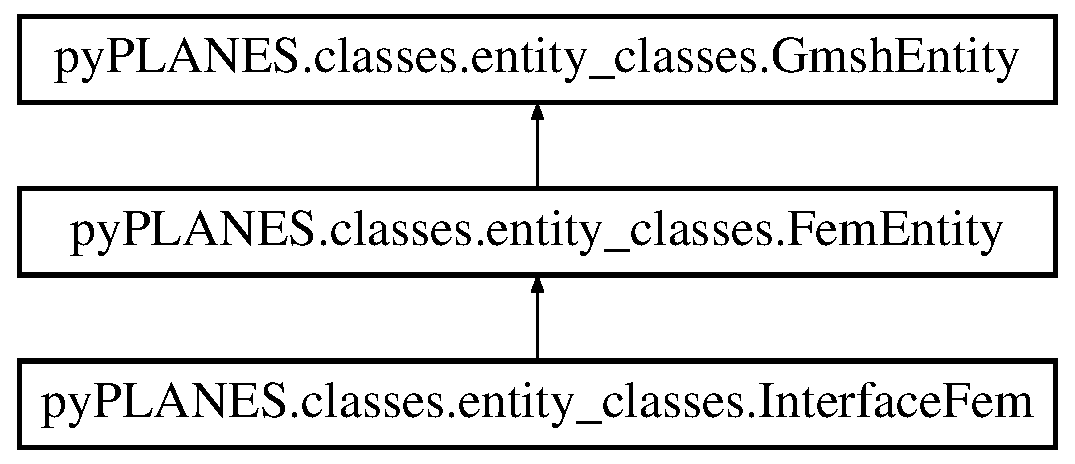
\includegraphics[height=3.000000cm]{classpy_p_l_a_n_e_s_1_1classes_1_1entity__classes_1_1_interface_fem}
\end{center}
\end{figure}
\subsection*{Public Member Functions}
\begin{DoxyCompactItemize}
\item 
\mbox{\Hypertarget{classpy_p_l_a_n_e_s_1_1classes_1_1entity__classes_1_1_interface_fem_a665daecfc7e625e9d8c44e0dbb1eca69}\label{classpy_p_l_a_n_e_s_1_1classes_1_1entity__classes_1_1_interface_fem_a665daecfc7e625e9d8c44e0dbb1eca69}} 
def {\bfseries \+\_\+\+\_\+init\+\_\+\+\_\+} (self, kwargs)
\item 
\mbox{\Hypertarget{classpy_p_l_a_n_e_s_1_1classes_1_1entity__classes_1_1_interface_fem_ab3b07eda6749c1306705aeaded78831b}\label{classpy_p_l_a_n_e_s_1_1classes_1_1entity__classes_1_1_interface_fem_ab3b07eda6749c1306705aeaded78831b}} 
def {\bfseries \+\_\+\+\_\+str\+\_\+\+\_\+} (self)
\item 
\mbox{\Hypertarget{classpy_p_l_a_n_e_s_1_1classes_1_1entity__classes_1_1_interface_fem_a4e86e4b7b127ebefaa2629f38c35d8cc}\label{classpy_p_l_a_n_e_s_1_1classes_1_1entity__classes_1_1_interface_fem_a4e86e4b7b127ebefaa2629f38c35d8cc}} 
def {\bfseries elementary\+\_\+matrices} (self, \+\_\+el)
\item 
\mbox{\Hypertarget{classpy_p_l_a_n_e_s_1_1classes_1_1entity__classes_1_1_interface_fem_a2c6a0791e2cc041d7ff35ad12a5985df}\label{classpy_p_l_a_n_e_s_1_1classes_1_1entity__classes_1_1_interface_fem_a2c6a0791e2cc041d7ff35ad12a5985df}} 
def {\bfseries append\+\_\+linear\+\_\+system} (self, omega)
\end{DoxyCompactItemize}
\subsection*{Public Attributes}
\begin{DoxyCompactItemize}
\item 
\mbox{\Hypertarget{classpy_p_l_a_n_e_s_1_1classes_1_1entity__classes_1_1_interface_fem_acdecea8fdcb355a5f49a9c80fac4812f}\label{classpy_p_l_a_n_e_s_1_1classes_1_1entity__classes_1_1_interface_fem_acdecea8fdcb355a5f49a9c80fac4812f}} 
{\bfseries ml}
\item 
\mbox{\Hypertarget{classpy_p_l_a_n_e_s_1_1classes_1_1entity__classes_1_1_interface_fem_a5d9c488496e682725300f8ba4d451846}\label{classpy_p_l_a_n_e_s_1_1classes_1_1entity__classes_1_1_interface_fem_a5d9c488496e682725300f8ba4d451846}} 
{\bfseries side}
\item 
\mbox{\Hypertarget{classpy_p_l_a_n_e_s_1_1classes_1_1entity__classes_1_1_interface_fem_a834937e0475167da27ac376c33556ea6}\label{classpy_p_l_a_n_e_s_1_1classes_1_1entity__classes_1_1_interface_fem_a834937e0475167da27ac376c33556ea6}} 
{\bfseries neighbour}
\item 
\mbox{\Hypertarget{classpy_p_l_a_n_e_s_1_1classes_1_1entity__classes_1_1_interface_fem_a74174476572b552729fd4875735ea32c}\label{classpy_p_l_a_n_e_s_1_1classes_1_1entity__classes_1_1_interface_fem_a74174476572b552729fd4875735ea32c}} 
{\bfseries nodes}
\end{DoxyCompactItemize}


The documentation for this class was generated from the following file\+:\begin{DoxyCompactItemize}
\item 
py\+P\+L\+A\+N\+E\+S/classes/entity\+\_\+classes.\+py\end{DoxyCompactItemize}

\hypertarget{classpy_p_l_a_n_e_s_1_1fem_1_1elements_1_1reference__elements_1_1_ka}{}\section{py\+P\+L\+A\+N\+E\+S.\+fem.\+elements.\+reference\+\_\+elements.\+Ka Class Reference}
\label{classpy_p_l_a_n_e_s_1_1fem_1_1elements_1_1reference__elements_1_1_ka}\index{py\+P\+L\+A\+N\+E\+S.\+fem.\+elements.\+reference\+\_\+elements.\+Ka@{py\+P\+L\+A\+N\+E\+S.\+fem.\+elements.\+reference\+\_\+elements.\+Ka}}
Inheritance diagram for py\+P\+L\+A\+N\+E\+S.\+fem.\+elements.\+reference\+\_\+elements.\+Ka\+:\begin{figure}[H]
\begin{center}
\leavevmode
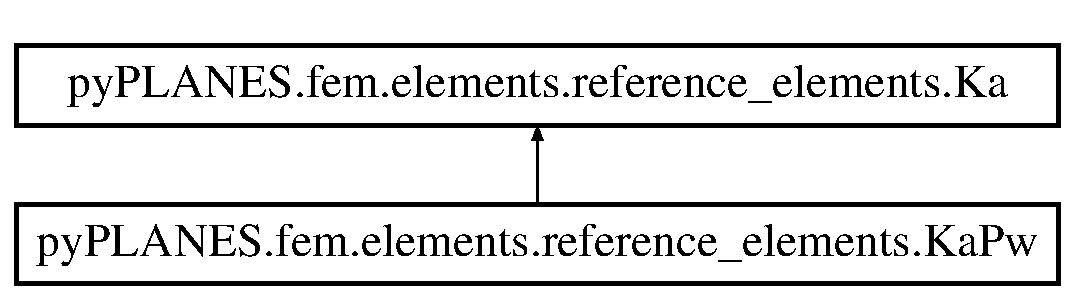
\includegraphics[height=2.000000cm]{classpy_p_l_a_n_e_s_1_1fem_1_1elements_1_1reference__elements_1_1_ka}
\end{center}
\end{figure}
\subsection*{Public Member Functions}
\begin{DoxyCompactItemize}
\item 
\mbox{\Hypertarget{classpy_p_l_a_n_e_s_1_1fem_1_1elements_1_1reference__elements_1_1_ka_aa84d62a2568dc8adbb70518e94cedfcd}\label{classpy_p_l_a_n_e_s_1_1fem_1_1elements_1_1reference__elements_1_1_ka_aa84d62a2568dc8adbb70518e94cedfcd}} 
def {\bfseries \+\_\+\+\_\+init\+\_\+\+\_\+} (self, order=2, p=4)
\item 
\mbox{\Hypertarget{classpy_p_l_a_n_e_s_1_1fem_1_1elements_1_1reference__elements_1_1_ka_a98008c414e90180338adb6cdf8327e29}\label{classpy_p_l_a_n_e_s_1_1fem_1_1elements_1_1reference__elements_1_1_ka_a98008c414e90180338adb6cdf8327e29}} 
def {\bfseries \+\_\+\+\_\+str\+\_\+\+\_\+} (self)
\end{DoxyCompactItemize}
\subsection*{Public Attributes}
\begin{DoxyCompactItemize}
\item 
\mbox{\Hypertarget{classpy_p_l_a_n_e_s_1_1fem_1_1elements_1_1reference__elements_1_1_ka_a1973a0da18e59cc0974a98b45d03610e}\label{classpy_p_l_a_n_e_s_1_1fem_1_1elements_1_1reference__elements_1_1_ka_a1973a0da18e59cc0974a98b45d03610e}} 
{\bfseries order}
\item 
\mbox{\Hypertarget{classpy_p_l_a_n_e_s_1_1fem_1_1elements_1_1reference__elements_1_1_ka_aabf940be4336c645e5ee343f8ca809a0}\label{classpy_p_l_a_n_e_s_1_1fem_1_1elements_1_1reference__elements_1_1_ka_aabf940be4336c645e5ee343f8ca809a0}} 
{\bfseries w}
\item 
\mbox{\Hypertarget{classpy_p_l_a_n_e_s_1_1fem_1_1elements_1_1reference__elements_1_1_ka_a9651efc5ee9e429a64ba2a6b95a6b3ec}\label{classpy_p_l_a_n_e_s_1_1fem_1_1elements_1_1reference__elements_1_1_ka_a9651efc5ee9e429a64ba2a6b95a6b3ec}} 
{\bfseries nb\+\_\+v}
\item 
\mbox{\Hypertarget{classpy_p_l_a_n_e_s_1_1fem_1_1elements_1_1reference__elements_1_1_ka_a3b3d6f98f73ce2062c5de8bdd89785b8}\label{classpy_p_l_a_n_e_s_1_1fem_1_1elements_1_1reference__elements_1_1_ka_a3b3d6f98f73ce2062c5de8bdd89785b8}} 
{\bfseries nb\+\_\+e}
\item 
\mbox{\Hypertarget{classpy_p_l_a_n_e_s_1_1fem_1_1elements_1_1reference__elements_1_1_ka_aaf1e1adc6f9e29d8e97889962314f5f8}\label{classpy_p_l_a_n_e_s_1_1fem_1_1elements_1_1reference__elements_1_1_ka_aaf1e1adc6f9e29d8e97889962314f5f8}} 
{\bfseries nb\+\_\+\+SF}
\item 
\mbox{\Hypertarget{classpy_p_l_a_n_e_s_1_1fem_1_1elements_1_1reference__elements_1_1_ka_a22796a4eab40a49097878eafd76a7281}\label{classpy_p_l_a_n_e_s_1_1fem_1_1elements_1_1reference__elements_1_1_ka_a22796a4eab40a49097878eafd76a7281}} 
{\bfseries Phi}
\item 
\mbox{\Hypertarget{classpy_p_l_a_n_e_s_1_1fem_1_1elements_1_1reference__elements_1_1_ka_af114ddb55705f43e8daa37bc62580add}\label{classpy_p_l_a_n_e_s_1_1fem_1_1elements_1_1reference__elements_1_1_ka_af114ddb55705f43e8daa37bc62580add}} 
{\bfseries d\+Phi}
\end{DoxyCompactItemize}


The documentation for this class was generated from the following file\+:\begin{DoxyCompactItemize}
\item 
py\+P\+L\+A\+N\+E\+S/fem/elements/reference\+\_\+elements.\+py\end{DoxyCompactItemize}

\hypertarget{classpy_p_l_a_n_e_s_1_1fem_1_1elements_1_1reference__elements_1_1_ka_pw}{}\section{py\+P\+L\+A\+N\+E\+S.\+fem.\+elements.\+reference\+\_\+elements.\+Ka\+Pw Class Reference}
\label{classpy_p_l_a_n_e_s_1_1fem_1_1elements_1_1reference__elements_1_1_ka_pw}\index{py\+P\+L\+A\+N\+E\+S.\+fem.\+elements.\+reference\+\_\+elements.\+Ka\+Pw@{py\+P\+L\+A\+N\+E\+S.\+fem.\+elements.\+reference\+\_\+elements.\+Ka\+Pw}}
Inheritance diagram for py\+P\+L\+A\+N\+E\+S.\+fem.\+elements.\+reference\+\_\+elements.\+Ka\+Pw\+:\begin{figure}[H]
\begin{center}
\leavevmode
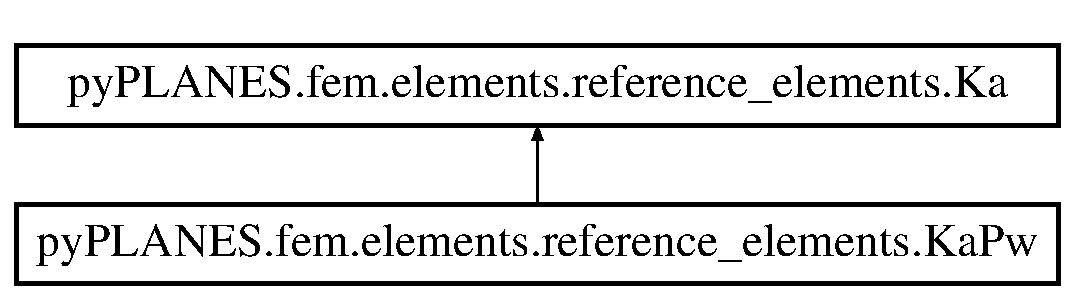
\includegraphics[height=2.000000cm]{classpy_p_l_a_n_e_s_1_1fem_1_1elements_1_1reference__elements_1_1_ka_pw}
\end{center}
\end{figure}
\subsection*{Public Member Functions}
\begin{DoxyCompactItemize}
\item 
\mbox{\Hypertarget{classpy_p_l_a_n_e_s_1_1fem_1_1elements_1_1reference__elements_1_1_ka_pw_a03e6f12c436eaba31d4de7fcc7f23b0d}\label{classpy_p_l_a_n_e_s_1_1fem_1_1elements_1_1reference__elements_1_1_ka_pw_a03e6f12c436eaba31d4de7fcc7f23b0d}} 
def {\bfseries \+\_\+\+\_\+init\+\_\+\+\_\+} (self, order=2, p=4)
\item 
\mbox{\Hypertarget{classpy_p_l_a_n_e_s_1_1fem_1_1elements_1_1reference__elements_1_1_ka_pw_a937d49ce67fa847f5879c3318781de7d}\label{classpy_p_l_a_n_e_s_1_1fem_1_1elements_1_1reference__elements_1_1_ka_pw_a937d49ce67fa847f5879c3318781de7d}} 
def {\bfseries \+\_\+\+\_\+str\+\_\+\+\_\+} (self)
\item 
def \mbox{\hyperlink{classpy_p_l_a_n_e_s_1_1fem_1_1elements_1_1reference__elements_1_1_ka_pw_ad87153ff42e7a432a2922bb67ac7b7be}{int\+\_\+lobatto\+\_\+exponential}} (self, k)
\end{DoxyCompactItemize}
\subsection*{Public Attributes}
\begin{DoxyCompactItemize}
\item 
\mbox{\Hypertarget{classpy_p_l_a_n_e_s_1_1fem_1_1elements_1_1reference__elements_1_1_ka_pw_a90571945e1cb1e11ea5eb5df8e703771}\label{classpy_p_l_a_n_e_s_1_1fem_1_1elements_1_1reference__elements_1_1_ka_pw_a90571945e1cb1e11ea5eb5df8e703771}} 
{\bfseries legendre\+\_\+table}
\end{DoxyCompactItemize}


\subsection{Member Function Documentation}
\mbox{\Hypertarget{classpy_p_l_a_n_e_s_1_1fem_1_1elements_1_1reference__elements_1_1_ka_pw_ad87153ff42e7a432a2922bb67ac7b7be}\label{classpy_p_l_a_n_e_s_1_1fem_1_1elements_1_1reference__elements_1_1_ka_pw_ad87153ff42e7a432a2922bb67ac7b7be}} 
\index{py\+P\+L\+A\+N\+E\+S\+::fem\+::elements\+::reference\+\_\+elements\+::\+Ka\+Pw@{py\+P\+L\+A\+N\+E\+S\+::fem\+::elements\+::reference\+\_\+elements\+::\+Ka\+Pw}!int\+\_\+lobatto\+\_\+exponential@{int\+\_\+lobatto\+\_\+exponential}}
\index{int\+\_\+lobatto\+\_\+exponential@{int\+\_\+lobatto\+\_\+exponential}!py\+P\+L\+A\+N\+E\+S\+::fem\+::elements\+::reference\+\_\+elements\+::\+Ka\+Pw@{py\+P\+L\+A\+N\+E\+S\+::fem\+::elements\+::reference\+\_\+elements\+::\+Ka\+Pw}}
\subsubsection{\texorpdfstring{int\+\_\+lobatto\+\_\+exponential()}{int\_lobatto\_exponential()}}
{\footnotesize\ttfamily def py\+P\+L\+A\+N\+E\+S.\+fem.\+elements.\+reference\+\_\+elements.\+Ka\+Pw.\+int\+\_\+lobatto\+\_\+exponential (\begin{DoxyParamCaption}\item[{}]{self,  }\item[{}]{k }\end{DoxyParamCaption})}

\begin{DoxyVerb}Returns the vector of \dint{-1}{1} ln(xi)e^{-ik xi} dxi\end{DoxyVerb}
 

The documentation for this class was generated from the following file\+:\begin{DoxyCompactItemize}
\item 
py\+P\+L\+A\+N\+E\+S/fem/elements/reference\+\_\+elements.\+py\end{DoxyCompactItemize}

\hypertarget{classpy_p_l_a_n_e_s_1_1fem_1_1elements_1_1reference__elements_1_1_kt}{}\section{py\+P\+L\+A\+N\+E\+S.\+fem.\+elements.\+reference\+\_\+elements.\+Kt Class Reference}
\label{classpy_p_l_a_n_e_s_1_1fem_1_1elements_1_1reference__elements_1_1_kt}\index{py\+P\+L\+A\+N\+E\+S.\+fem.\+elements.\+reference\+\_\+elements.\+Kt@{py\+P\+L\+A\+N\+E\+S.\+fem.\+elements.\+reference\+\_\+elements.\+Kt}}
\subsection*{Public Member Functions}
\begin{DoxyCompactItemize}
\item 
\mbox{\Hypertarget{classpy_p_l_a_n_e_s_1_1fem_1_1elements_1_1reference__elements_1_1_kt_ae6aff9e2f860ac0bcef13cf04d2b42bb}\label{classpy_p_l_a_n_e_s_1_1fem_1_1elements_1_1reference__elements_1_1_kt_ae6aff9e2f860ac0bcef13cf04d2b42bb}} 
def {\bfseries \+\_\+\+\_\+init\+\_\+\+\_\+} (self, order=2, p=4)
\item 
\mbox{\Hypertarget{classpy_p_l_a_n_e_s_1_1fem_1_1elements_1_1reference__elements_1_1_kt_ab207b5573d30fb7eb26809fc04cbf181}\label{classpy_p_l_a_n_e_s_1_1fem_1_1elements_1_1reference__elements_1_1_kt_ab207b5573d30fb7eb26809fc04cbf181}} 
def {\bfseries \+\_\+\+\_\+str\+\_\+\+\_\+} (self)
\end{DoxyCompactItemize}
\subsection*{Public Attributes}
\begin{DoxyCompactItemize}
\item 
\mbox{\Hypertarget{classpy_p_l_a_n_e_s_1_1fem_1_1elements_1_1reference__elements_1_1_kt_ad49cea824c0dbc5541be6fac0c68bc3f}\label{classpy_p_l_a_n_e_s_1_1fem_1_1elements_1_1reference__elements_1_1_kt_ad49cea824c0dbc5541be6fac0c68bc3f}} 
{\bfseries order}
\item 
\mbox{\Hypertarget{classpy_p_l_a_n_e_s_1_1fem_1_1elements_1_1reference__elements_1_1_kt_af73486c0ebbddd17b02c04d9e2f005c3}\label{classpy_p_l_a_n_e_s_1_1fem_1_1elements_1_1reference__elements_1_1_kt_af73486c0ebbddd17b02c04d9e2f005c3}} 
{\bfseries w}
\item 
\mbox{\Hypertarget{classpy_p_l_a_n_e_s_1_1fem_1_1elements_1_1reference__elements_1_1_kt_a418ab776b9a4e26d0af6641b5c33270e}\label{classpy_p_l_a_n_e_s_1_1fem_1_1elements_1_1reference__elements_1_1_kt_a418ab776b9a4e26d0af6641b5c33270e}} 
{\bfseries nb\+\_\+v}
\item 
\mbox{\Hypertarget{classpy_p_l_a_n_e_s_1_1fem_1_1elements_1_1reference__elements_1_1_kt_a48a25b3057bd9ff981854830212144b9}\label{classpy_p_l_a_n_e_s_1_1fem_1_1elements_1_1reference__elements_1_1_kt_a48a25b3057bd9ff981854830212144b9}} 
{\bfseries nb\+\_\+e}
\item 
\mbox{\Hypertarget{classpy_p_l_a_n_e_s_1_1fem_1_1elements_1_1reference__elements_1_1_kt_a2b400a75e1210f87faedccd43d8abf59}\label{classpy_p_l_a_n_e_s_1_1fem_1_1elements_1_1reference__elements_1_1_kt_a2b400a75e1210f87faedccd43d8abf59}} 
{\bfseries nb\+\_\+f}
\item 
\mbox{\Hypertarget{classpy_p_l_a_n_e_s_1_1fem_1_1elements_1_1reference__elements_1_1_kt_a905ccb5d247270e5643bf124c6eb4c97}\label{classpy_p_l_a_n_e_s_1_1fem_1_1elements_1_1reference__elements_1_1_kt_a905ccb5d247270e5643bf124c6eb4c97}} 
{\bfseries nb\+\_\+m\+\_\+\+SF}
\item 
\mbox{\Hypertarget{classpy_p_l_a_n_e_s_1_1fem_1_1elements_1_1reference__elements_1_1_kt_a7ade4a75e9f311ceaf8a61143724a6f7}\label{classpy_p_l_a_n_e_s_1_1fem_1_1elements_1_1reference__elements_1_1_kt_a7ade4a75e9f311ceaf8a61143724a6f7}} 
{\bfseries nb\+\_\+s\+\_\+\+SF}
\item 
\mbox{\Hypertarget{classpy_p_l_a_n_e_s_1_1fem_1_1elements_1_1reference__elements_1_1_kt_adcc8503be5fb181a48a12f891348ab8f}\label{classpy_p_l_a_n_e_s_1_1fem_1_1elements_1_1reference__elements_1_1_kt_adcc8503be5fb181a48a12f891348ab8f}} 
{\bfseries nb\+\_\+\+SF}
\item 
\mbox{\Hypertarget{classpy_p_l_a_n_e_s_1_1fem_1_1elements_1_1reference__elements_1_1_kt_a1f64cead6e00d91f590c9ce2b4b27104}\label{classpy_p_l_a_n_e_s_1_1fem_1_1elements_1_1reference__elements_1_1_kt_a1f64cead6e00d91f590c9ce2b4b27104}} 
{\bfseries d\+Phi}
\item 
\mbox{\Hypertarget{classpy_p_l_a_n_e_s_1_1fem_1_1elements_1_1reference__elements_1_1_kt_abb547d828cef870c93dda85a6191c29d}\label{classpy_p_l_a_n_e_s_1_1fem_1_1elements_1_1reference__elements_1_1_kt_abb547d828cef870c93dda85a6191c29d}} 
{\bfseries phi\+\_\+plot}
\end{DoxyCompactItemize}


The documentation for this class was generated from the following file\+:\begin{DoxyCompactItemize}
\item 
py\+P\+L\+A\+N\+E\+S/fem/elements/reference\+\_\+elements.\+py\end{DoxyCompactItemize}

\hypertarget{classpy_p_l_a_n_e_s_1_1gmsh_1_1write__geo__file_1_1_gmsh_1_1_line}{}\section{py\+P\+L\+A\+N\+E\+S.\+gmsh.\+write\+\_\+geo\+\_\+file.\+Gmsh.\+Line Class Reference}
\label{classpy_p_l_a_n_e_s_1_1gmsh_1_1write__geo__file_1_1_gmsh_1_1_line}\index{py\+P\+L\+A\+N\+E\+S.\+gmsh.\+write\+\_\+geo\+\_\+file.\+Gmsh.\+Line@{py\+P\+L\+A\+N\+E\+S.\+gmsh.\+write\+\_\+geo\+\_\+file.\+Gmsh.\+Line}}
\subsection*{Public Member Functions}
\begin{DoxyCompactItemize}
\item 
\mbox{\Hypertarget{classpy_p_l_a_n_e_s_1_1gmsh_1_1write__geo__file_1_1_gmsh_1_1_line_aa874eb1a6a65ad823e32122bb19c5f1f}\label{classpy_p_l_a_n_e_s_1_1gmsh_1_1write__geo__file_1_1_gmsh_1_1_line_aa874eb1a6a65ad823e32122bb19c5f1f}} 
def {\bfseries \+\_\+\+\_\+init\+\_\+\+\_\+} (self, f, tag, \+\_\+1, \+\_\+2)
\item 
\mbox{\Hypertarget{classpy_p_l_a_n_e_s_1_1gmsh_1_1write__geo__file_1_1_gmsh_1_1_line_af48c6f47351a12d11cc1a2c98bd307fc}\label{classpy_p_l_a_n_e_s_1_1gmsh_1_1write__geo__file_1_1_gmsh_1_1_line_af48c6f47351a12d11cc1a2c98bd307fc}} 
def {\bfseries \+\_\+\+\_\+str\+\_\+\+\_\+} (self)
\item 
\mbox{\Hypertarget{classpy_p_l_a_n_e_s_1_1gmsh_1_1write__geo__file_1_1_gmsh_1_1_line_a920dfb84ec2527f1850d80ca2b7d3eab}\label{classpy_p_l_a_n_e_s_1_1gmsh_1_1write__geo__file_1_1_gmsh_1_1_line_a920dfb84ec2527f1850d80ca2b7d3eab}} 
def {\bfseries inverted} (self)
\end{DoxyCompactItemize}
\subsection*{Public Attributes}
\begin{DoxyCompactItemize}
\item 
\mbox{\Hypertarget{classpy_p_l_a_n_e_s_1_1gmsh_1_1write__geo__file_1_1_gmsh_1_1_line_adcda2a8007b6a36c36cf9863db3dc5f1}\label{classpy_p_l_a_n_e_s_1_1gmsh_1_1write__geo__file_1_1_gmsh_1_1_line_adcda2a8007b6a36c36cf9863db3dc5f1}} 
{\bfseries p\+\_\+1}
\item 
\mbox{\Hypertarget{classpy_p_l_a_n_e_s_1_1gmsh_1_1write__geo__file_1_1_gmsh_1_1_line_aeb1d41f6d209acd442fcb89ff605d064}\label{classpy_p_l_a_n_e_s_1_1gmsh_1_1write__geo__file_1_1_gmsh_1_1_line_aeb1d41f6d209acd442fcb89ff605d064}} 
{\bfseries p\+\_\+2}
\item 
\mbox{\Hypertarget{classpy_p_l_a_n_e_s_1_1gmsh_1_1write__geo__file_1_1_gmsh_1_1_line_a4a63127c1e595dad350d003ed3896ac7}\label{classpy_p_l_a_n_e_s_1_1gmsh_1_1write__geo__file_1_1_gmsh_1_1_line_a4a63127c1e595dad350d003ed3896ac7}} 
{\bfseries tag}
\item 
\mbox{\Hypertarget{classpy_p_l_a_n_e_s_1_1gmsh_1_1write__geo__file_1_1_gmsh_1_1_line_a29360f0474a216664b445c6fd9fc2ce9}\label{classpy_p_l_a_n_e_s_1_1gmsh_1_1write__geo__file_1_1_gmsh_1_1_line_a29360f0474a216664b445c6fd9fc2ce9}} 
{\bfseries typ}
\end{DoxyCompactItemize}


The documentation for this class was generated from the following file\+:\begin{DoxyCompactItemize}
\item 
py\+P\+L\+A\+N\+E\+S/gmsh/write\+\_\+geo\+\_\+file.\+py\end{DoxyCompactItemize}

\hypertarget{classpy_p_l_a_n_e_s_1_1gmsh_1_1write__geo__file_1_1_gmsh_1_1_line_loop}{}\section{py\+P\+L\+A\+N\+E\+S.\+gmsh.\+write\+\_\+geo\+\_\+file.\+Gmsh.\+Line\+Loop Class Reference}
\label{classpy_p_l_a_n_e_s_1_1gmsh_1_1write__geo__file_1_1_gmsh_1_1_line_loop}\index{py\+P\+L\+A\+N\+E\+S.\+gmsh.\+write\+\_\+geo\+\_\+file.\+Gmsh.\+Line\+Loop@{py\+P\+L\+A\+N\+E\+S.\+gmsh.\+write\+\_\+geo\+\_\+file.\+Gmsh.\+Line\+Loop}}
\subsection*{Public Member Functions}
\begin{DoxyCompactItemize}
\item 
\mbox{\Hypertarget{classpy_p_l_a_n_e_s_1_1gmsh_1_1write__geo__file_1_1_gmsh_1_1_line_loop_a1e86a55f796a06fdb3a50084715112ea}\label{classpy_p_l_a_n_e_s_1_1gmsh_1_1write__geo__file_1_1_gmsh_1_1_line_loop_a1e86a55f796a06fdb3a50084715112ea}} 
def {\bfseries \+\_\+\+\_\+init\+\_\+\+\_\+} (self, f, tag, \+\_\+list)
\end{DoxyCompactItemize}
\subsection*{Public Attributes}
\begin{DoxyCompactItemize}
\item 
\mbox{\Hypertarget{classpy_p_l_a_n_e_s_1_1gmsh_1_1write__geo__file_1_1_gmsh_1_1_line_loop_ab2f8182cd5bd3f05a55cd5f7cc61c0b7}\label{classpy_p_l_a_n_e_s_1_1gmsh_1_1write__geo__file_1_1_gmsh_1_1_line_loop_ab2f8182cd5bd3f05a55cd5f7cc61c0b7}} 
{\bfseries lines}
\item 
\mbox{\Hypertarget{classpy_p_l_a_n_e_s_1_1gmsh_1_1write__geo__file_1_1_gmsh_1_1_line_loop_a3498e769049290734f535583233a33ee}\label{classpy_p_l_a_n_e_s_1_1gmsh_1_1write__geo__file_1_1_gmsh_1_1_line_loop_a3498e769049290734f535583233a33ee}} 
{\bfseries tag}
\item 
\mbox{\Hypertarget{classpy_p_l_a_n_e_s_1_1gmsh_1_1write__geo__file_1_1_gmsh_1_1_line_loop_ab588405c5f5f48bbfd27766090292e8d}\label{classpy_p_l_a_n_e_s_1_1gmsh_1_1write__geo__file_1_1_gmsh_1_1_line_loop_ab588405c5f5f48bbfd27766090292e8d}} 
{\bfseries typ}
\end{DoxyCompactItemize}


The documentation for this class was generated from the following file\+:\begin{DoxyCompactItemize}
\item 
py\+P\+L\+A\+N\+E\+S/gmsh/write\+\_\+geo\+\_\+file.\+py\end{DoxyCompactItemize}

\hypertarget{classpy_p_l_a_n_e_s_1_1classes_1_1mesh_1_1_mesh}{}\section{py\+P\+L\+A\+N\+E\+S.\+classes.\+mesh.\+Mesh Class Reference}
\label{classpy_p_l_a_n_e_s_1_1classes_1_1mesh_1_1_mesh}\index{py\+P\+L\+A\+N\+E\+S.\+classes.\+mesh.\+Mesh@{py\+P\+L\+A\+N\+E\+S.\+classes.\+mesh.\+Mesh}}
Inheritance diagram for py\+P\+L\+A\+N\+E\+S.\+classes.\+mesh.\+Mesh\+:\begin{figure}[H]
\begin{center}
\leavevmode
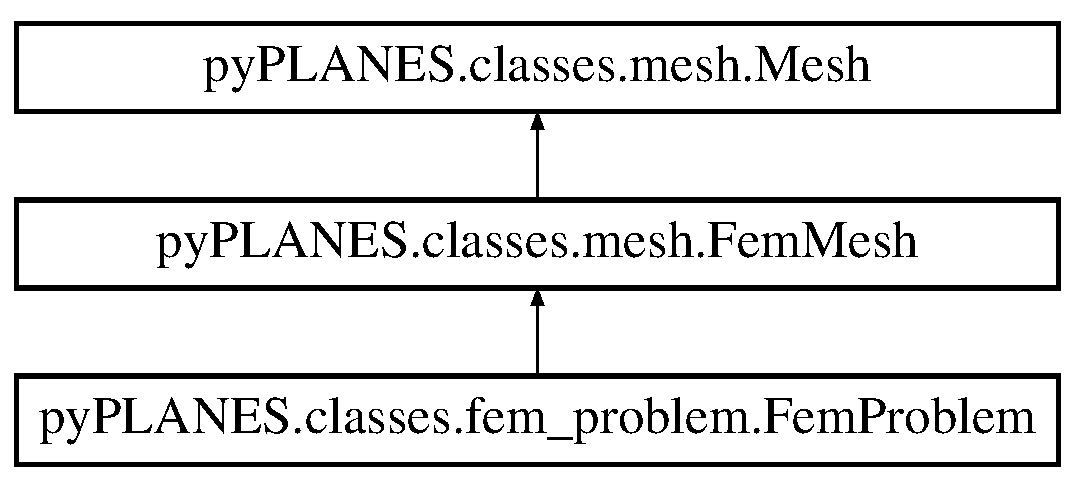
\includegraphics[height=3.000000cm]{classpy_p_l_a_n_e_s_1_1classes_1_1mesh_1_1_mesh}
\end{center}
\end{figure}
\subsection*{Public Member Functions}
\begin{DoxyCompactItemize}
\item 
\mbox{\Hypertarget{classpy_p_l_a_n_e_s_1_1classes_1_1mesh_1_1_mesh_a36ee9e8746e4cc5bda5f6ef8c1c0515a}\label{classpy_p_l_a_n_e_s_1_1classes_1_1mesh_1_1_mesh_a36ee9e8746e4cc5bda5f6ef8c1c0515a}} 
def {\bfseries \+\_\+\+\_\+init\+\_\+\+\_\+} (self, kwargs)
\end{DoxyCompactItemize}
\subsection*{Public Attributes}
\begin{DoxyCompactItemize}
\item 
\mbox{\Hypertarget{classpy_p_l_a_n_e_s_1_1classes_1_1mesh_1_1_mesh_ac15122ee911d9b9c915487caa7922cc5}\label{classpy_p_l_a_n_e_s_1_1classes_1_1mesh_1_1_mesh_ac15122ee911d9b9c915487caa7922cc5}} 
{\bfseries entities}
\item 
\mbox{\Hypertarget{classpy_p_l_a_n_e_s_1_1classes_1_1mesh_1_1_mesh_aea1bc352a27baadbdaaac62c5bc23ccd}\label{classpy_p_l_a_n_e_s_1_1classes_1_1mesh_1_1_mesh_aea1bc352a27baadbdaaac62c5bc23ccd}} 
{\bfseries model\+\_\+entities}
\item 
\mbox{\Hypertarget{classpy_p_l_a_n_e_s_1_1classes_1_1mesh_1_1_mesh_afd1d2275ddbe3ddcad7fcb334e086c46}\label{classpy_p_l_a_n_e_s_1_1classes_1_1mesh_1_1_mesh_afd1d2275ddbe3ddcad7fcb334e086c46}} 
{\bfseries vertices}
\item 
\mbox{\Hypertarget{classpy_p_l_a_n_e_s_1_1classes_1_1mesh_1_1_mesh_ac4ee3f9b3a0ceb423f2952f49db2f07e}\label{classpy_p_l_a_n_e_s_1_1classes_1_1mesh_1_1_mesh_ac4ee3f9b3a0ceb423f2952f49db2f07e}} 
{\bfseries elements}
\item 
\mbox{\Hypertarget{classpy_p_l_a_n_e_s_1_1classes_1_1mesh_1_1_mesh_a92837406d5a6161d2931c61cbb2be046}\label{classpy_p_l_a_n_e_s_1_1classes_1_1mesh_1_1_mesh_a92837406d5a6161d2931c61cbb2be046}} 
{\bfseries materials\+\_\+directory}
\item 
\mbox{\Hypertarget{classpy_p_l_a_n_e_s_1_1classes_1_1mesh_1_1_mesh_a07f6b8becc41cf582ec7ff6d07563ea2}\label{classpy_p_l_a_n_e_s_1_1classes_1_1mesh_1_1_mesh_a07f6b8becc41cf582ec7ff6d07563ea2}} 
{\bfseries reference\+\_\+elements}
\end{DoxyCompactItemize}


The documentation for this class was generated from the following file\+:\begin{DoxyCompactItemize}
\item 
py\+P\+L\+A\+N\+E\+S/classes/mesh.\+py\end{DoxyCompactItemize}

\hypertarget{classpy_p_l_a_n_e_s_1_1classes_1_1model_1_1_model}{}\section{py\+P\+L\+A\+N\+E\+S.\+classes.\+model.\+Model Class Reference}
\label{classpy_p_l_a_n_e_s_1_1classes_1_1model_1_1_model}\index{py\+P\+L\+A\+N\+E\+S.\+classes.\+model.\+Model@{py\+P\+L\+A\+N\+E\+S.\+classes.\+model.\+Model}}
Inheritance diagram for py\+P\+L\+A\+N\+E\+S.\+classes.\+model.\+Model\+:\begin{figure}[H]
\begin{center}
\leavevmode
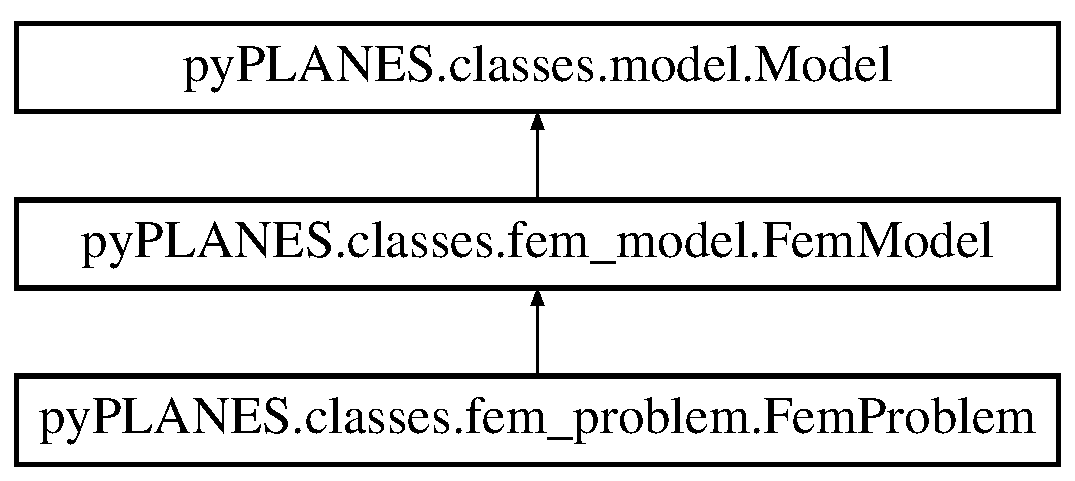
\includegraphics[height=3.000000cm]{classpy_p_l_a_n_e_s_1_1classes_1_1model_1_1_model}
\end{center}
\end{figure}
\subsection*{Public Member Functions}
\begin{DoxyCompactItemize}
\item 
\mbox{\Hypertarget{classpy_p_l_a_n_e_s_1_1classes_1_1model_1_1_model_af058d898b31594bb77c79503a03e14d4}\label{classpy_p_l_a_n_e_s_1_1classes_1_1model_1_1_model_af058d898b31594bb77c79503a03e14d4}} 
def {\bfseries \+\_\+\+\_\+init\+\_\+\+\_\+} (self, kwargs)
\item 
\mbox{\Hypertarget{classpy_p_l_a_n_e_s_1_1classes_1_1model_1_1_model_a9c95d1e15f792b3d3add5941f9afa417}\label{classpy_p_l_a_n_e_s_1_1classes_1_1model_1_1_model_a9c95d1e15f792b3d3add5941f9afa417}} 
def {\bfseries extend\+\_\+\+AF} (self, \+\_\+\+A\+\_\+i, \+\_\+\+A\+\_\+j, \+\_\+\+A\+\_\+v, \+\_\+\+F\+\_\+i, \+\_\+\+F\+\_\+v)
\item 
\mbox{\Hypertarget{classpy_p_l_a_n_e_s_1_1classes_1_1model_1_1_model_a60d16f0a4f3cc09662bcdbe01dafc682}\label{classpy_p_l_a_n_e_s_1_1classes_1_1model_1_1_model_a60d16f0a4f3cc09662bcdbe01dafc682}} 
def {\bfseries extend\+\_\+F} (self, \+\_\+\+F\+\_\+i, \+\_\+\+F\+\_\+v)
\item 
\mbox{\Hypertarget{classpy_p_l_a_n_e_s_1_1classes_1_1model_1_1_model_ab69f59761ed14ab310c70dac7866e974}\label{classpy_p_l_a_n_e_s_1_1classes_1_1model_1_1_model_ab69f59761ed14ab310c70dac7866e974}} 
def {\bfseries extend\+\_\+A} (self, \+\_\+\+A\+\_\+i, \+\_\+\+A\+\_\+j, \+\_\+\+A\+\_\+v)
\item 
\mbox{\Hypertarget{classpy_p_l_a_n_e_s_1_1classes_1_1model_1_1_model_a0eb2e6f6b6cddfbc5c455def5d5cf0e2}\label{classpy_p_l_a_n_e_s_1_1classes_1_1model_1_1_model_a0eb2e6f6b6cddfbc5c455def5d5cf0e2}} 
def {\bfseries extend\+\_\+\+A\+\_\+\+F\+\_\+from\+\_\+coo} (self, AF)
\item 
\mbox{\Hypertarget{classpy_p_l_a_n_e_s_1_1classes_1_1model_1_1_model_ad11afe301f5f718b4f746da4b778eca8}\label{classpy_p_l_a_n_e_s_1_1classes_1_1model_1_1_model_ad11afe301f5f718b4f746da4b778eca8}} 
def {\bfseries extend\+\_\+\+AT} (self, \+\_\+\+A\+\_\+i, \+\_\+\+A\+\_\+j, \+\_\+\+A\+\_\+v, \+\_\+\+T\+\_\+i, \+\_\+\+T\+\_\+j, \+\_\+\+T\+\_\+v)
\item 
\mbox{\Hypertarget{classpy_p_l_a_n_e_s_1_1classes_1_1model_1_1_model_a912097bb9b8a184432168b4fcfa03e11}\label{classpy_p_l_a_n_e_s_1_1classes_1_1model_1_1_model_a912097bb9b8a184432168b4fcfa03e11}} 
def {\bfseries linear\+\_\+system\+\_\+2\+\_\+numpy} (self)
\item 
\mbox{\Hypertarget{classpy_p_l_a_n_e_s_1_1classes_1_1model_1_1_model_a8ff7fbd319efe85a0dd729a9bc92c6c9}\label{classpy_p_l_a_n_e_s_1_1classes_1_1model_1_1_model_a8ff7fbd319efe85a0dd729a9bc92c6c9}} 
def {\bfseries write\+\_\+out\+\_\+files} (self)
\item 
\mbox{\Hypertarget{classpy_p_l_a_n_e_s_1_1classes_1_1model_1_1_model_a47eac14873bb55bc7ff3b72be856d64e}\label{classpy_p_l_a_n_e_s_1_1classes_1_1model_1_1_model_a47eac14873bb55bc7ff3b72be856d64e}} 
def {\bfseries create\+\_\+linear\+\_\+system} (self, f)
\item 
\mbox{\Hypertarget{classpy_p_l_a_n_e_s_1_1classes_1_1model_1_1_model_af7cd1c9cb7ac9d8380db8a8f7e54fb1b}\label{classpy_p_l_a_n_e_s_1_1classes_1_1model_1_1_model_af7cd1c9cb7ac9d8380db8a8f7e54fb1b}} 
def {\bfseries initialisation\+\_\+out\+\_\+files} (self)
\item 
\mbox{\Hypertarget{classpy_p_l_a_n_e_s_1_1classes_1_1model_1_1_model_a539272244c9eea5c8b3fd8101b354170}\label{classpy_p_l_a_n_e_s_1_1classes_1_1model_1_1_model_a539272244c9eea5c8b3fd8101b354170}} 
def {\bfseries close\+\_\+out\+\_\+files} (self)
\item 
\mbox{\Hypertarget{classpy_p_l_a_n_e_s_1_1classes_1_1model_1_1_model_ab981465eeff13c7a6823780c8df5bd64}\label{classpy_p_l_a_n_e_s_1_1classes_1_1model_1_1_model_ab981465eeff13c7a6823780c8df5bd64}} 
def {\bfseries resolution} (self)
\end{DoxyCompactItemize}
\subsection*{Public Attributes}
\begin{DoxyCompactItemize}
\item 
\mbox{\Hypertarget{classpy_p_l_a_n_e_s_1_1classes_1_1model_1_1_model_ae907e606a369b6e34d139247ac79d555}\label{classpy_p_l_a_n_e_s_1_1classes_1_1model_1_1_model_ae907e606a369b6e34d139247ac79d555}} 
{\bfseries plot}
\item 
\mbox{\Hypertarget{classpy_p_l_a_n_e_s_1_1classes_1_1model_1_1_model_af220822f3071ae1df209e8abc39b8884}\label{classpy_p_l_a_n_e_s_1_1classes_1_1model_1_1_model_af220822f3071ae1df209e8abc39b8884}} 
{\bfseries F\+\_\+i}
\item 
\mbox{\Hypertarget{classpy_p_l_a_n_e_s_1_1classes_1_1model_1_1_model_aee1987677d6e6b14addafdf0c1a49ff5}\label{classpy_p_l_a_n_e_s_1_1classes_1_1model_1_1_model_aee1987677d6e6b14addafdf0c1a49ff5}} 
{\bfseries F\+\_\+v}
\item 
\mbox{\Hypertarget{classpy_p_l_a_n_e_s_1_1classes_1_1model_1_1_model_a93996577615d4d6717f93b42032b0f50}\label{classpy_p_l_a_n_e_s_1_1classes_1_1model_1_1_model_a93996577615d4d6717f93b42032b0f50}} 
{\bfseries A\+\_\+i}
\item 
\mbox{\Hypertarget{classpy_p_l_a_n_e_s_1_1classes_1_1model_1_1_model_a83d62229044648b09d2cdd3eb75a4bad}\label{classpy_p_l_a_n_e_s_1_1classes_1_1model_1_1_model_a83d62229044648b09d2cdd3eb75a4bad}} 
{\bfseries A\+\_\+j}
\item 
\mbox{\Hypertarget{classpy_p_l_a_n_e_s_1_1classes_1_1model_1_1_model_a8c597b56cbbd022f1f16c09d2b4ca0ce}\label{classpy_p_l_a_n_e_s_1_1classes_1_1model_1_1_model_a8c597b56cbbd022f1f16c09d2b4ca0ce}} 
{\bfseries A\+\_\+v}
\item 
\mbox{\Hypertarget{classpy_p_l_a_n_e_s_1_1classes_1_1model_1_1_model_ae68c961988c3501fa63e9ad27abdd6e5}\label{classpy_p_l_a_n_e_s_1_1classes_1_1model_1_1_model_ae68c961988c3501fa63e9ad27abdd6e5}} 
{\bfseries T\+\_\+i}
\item 
\mbox{\Hypertarget{classpy_p_l_a_n_e_s_1_1classes_1_1model_1_1_model_abf6d2c66127f70d0290c470ad25d6c2b}\label{classpy_p_l_a_n_e_s_1_1classes_1_1model_1_1_model_abf6d2c66127f70d0290c470ad25d6c2b}} 
{\bfseries T\+\_\+j}
\item 
\mbox{\Hypertarget{classpy_p_l_a_n_e_s_1_1classes_1_1model_1_1_model_a6dc88c9b37fc8e245fa0d079ebf19653}\label{classpy_p_l_a_n_e_s_1_1classes_1_1model_1_1_model_a6dc88c9b37fc8e245fa0d079ebf19653}} 
{\bfseries T\+\_\+v}
\item 
\mbox{\Hypertarget{classpy_p_l_a_n_e_s_1_1classes_1_1model_1_1_model_af107d1782fb62471d9b31197f8d4f193}\label{classpy_p_l_a_n_e_s_1_1classes_1_1model_1_1_model_af107d1782fb62471d9b31197f8d4f193}} 
{\bfseries start\+\_\+time}
\end{DoxyCompactItemize}


The documentation for this class was generated from the following file\+:\begin{DoxyCompactItemize}
\item 
py\+P\+L\+A\+N\+E\+S/classes/model.\+py\end{DoxyCompactItemize}

\hypertarget{classpy_p_l_a_n_e_s_1_1classes_1_1entity__classes_1_1_pem_fem}{}\section{py\+P\+L\+A\+N\+E\+S.\+classes.\+entity\+\_\+classes.\+Pem\+Fem Class Reference}
\label{classpy_p_l_a_n_e_s_1_1classes_1_1entity__classes_1_1_pem_fem}\index{py\+P\+L\+A\+N\+E\+S.\+classes.\+entity\+\_\+classes.\+Pem\+Fem@{py\+P\+L\+A\+N\+E\+S.\+classes.\+entity\+\_\+classes.\+Pem\+Fem}}
Inheritance diagram for py\+P\+L\+A\+N\+E\+S.\+classes.\+entity\+\_\+classes.\+Pem\+Fem\+:\begin{figure}[H]
\begin{center}
\leavevmode
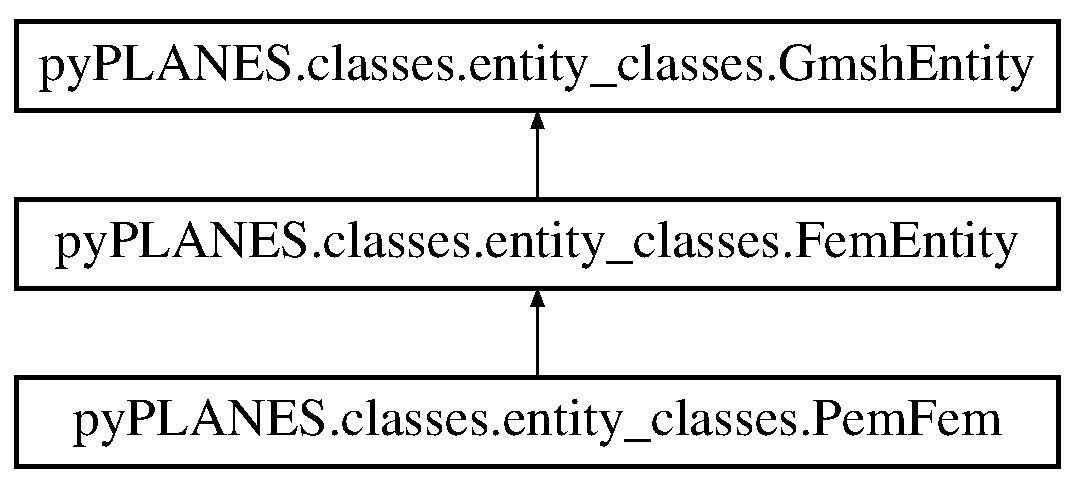
\includegraphics[height=3.000000cm]{classpy_p_l_a_n_e_s_1_1classes_1_1entity__classes_1_1_pem_fem}
\end{center}
\end{figure}
\subsection*{Public Member Functions}
\begin{DoxyCompactItemize}
\item 
\mbox{\Hypertarget{classpy_p_l_a_n_e_s_1_1classes_1_1entity__classes_1_1_pem_fem_af01b9f16713a054050250c6be7edd3cb}\label{classpy_p_l_a_n_e_s_1_1classes_1_1entity__classes_1_1_pem_fem_af01b9f16713a054050250c6be7edd3cb}} 
def {\bfseries \+\_\+\+\_\+init\+\_\+\+\_\+} (self, kwargs)
\item 
\mbox{\Hypertarget{classpy_p_l_a_n_e_s_1_1classes_1_1entity__classes_1_1_pem_fem_a76378d96d5a41bbedca95b8f996deb4f}\label{classpy_p_l_a_n_e_s_1_1classes_1_1entity__classes_1_1_pem_fem_a76378d96d5a41bbedca95b8f996deb4f}} 
def {\bfseries \+\_\+\+\_\+str\+\_\+\+\_\+} (self)
\item 
\mbox{\Hypertarget{classpy_p_l_a_n_e_s_1_1classes_1_1entity__classes_1_1_pem_fem_abd7d6d78db03b9ab7d76d8fb7469a649}\label{classpy_p_l_a_n_e_s_1_1classes_1_1entity__classes_1_1_pem_fem_abd7d6d78db03b9ab7d76d8fb7469a649}} 
def {\bfseries update\+\_\+frequency} (self, omega)
\item 
\mbox{\Hypertarget{classpy_p_l_a_n_e_s_1_1classes_1_1entity__classes_1_1_pem_fem_a716e2697308a20a478892d2abcc259da}\label{classpy_p_l_a_n_e_s_1_1classes_1_1entity__classes_1_1_pem_fem_a716e2697308a20a478892d2abcc259da}} 
def {\bfseries elementary\+\_\+matrices} (self, \+\_\+el)
\item 
\mbox{\Hypertarget{classpy_p_l_a_n_e_s_1_1classes_1_1entity__classes_1_1_pem_fem_a611e62b63ea32fc83225753d0661e66e}\label{classpy_p_l_a_n_e_s_1_1classes_1_1entity__classes_1_1_pem_fem_a611e62b63ea32fc83225753d0661e66e}} 
def {\bfseries append\+\_\+linear\+\_\+system} (self, omega)
\end{DoxyCompactItemize}
\subsection*{Public Attributes}
\begin{DoxyCompactItemize}
\item 
\mbox{\Hypertarget{classpy_p_l_a_n_e_s_1_1classes_1_1entity__classes_1_1_pem_fem_a905224aeca7b1ce94895db41b2609cf0}\label{classpy_p_l_a_n_e_s_1_1classes_1_1entity__classes_1_1_pem_fem_a905224aeca7b1ce94895db41b2609cf0}} 
{\bfseries mat}
\item 
\mbox{\Hypertarget{classpy_p_l_a_n_e_s_1_1classes_1_1entity__classes_1_1_pem_fem_a6ece1d38a0723e4be3f5d264eac57a29}\label{classpy_p_l_a_n_e_s_1_1classes_1_1entity__classes_1_1_pem_fem_a6ece1d38a0723e4be3f5d264eac57a29}} 
{\bfseries formulation98}
\end{DoxyCompactItemize}


The documentation for this class was generated from the following file\+:\begin{DoxyCompactItemize}
\item 
py\+P\+L\+A\+N\+E\+S/classes/entity\+\_\+classes.\+py\end{DoxyCompactItemize}

\hypertarget{classpy_p_l_a_n_e_s_1_1classes_1_1entity__classes_1_1_periodicity_fem}{}\section{py\+P\+L\+A\+N\+E\+S.\+classes.\+entity\+\_\+classes.\+Periodicity\+Fem Class Reference}
\label{classpy_p_l_a_n_e_s_1_1classes_1_1entity__classes_1_1_periodicity_fem}\index{py\+P\+L\+A\+N\+E\+S.\+classes.\+entity\+\_\+classes.\+Periodicity\+Fem@{py\+P\+L\+A\+N\+E\+S.\+classes.\+entity\+\_\+classes.\+Periodicity\+Fem}}
Inheritance diagram for py\+P\+L\+A\+N\+E\+S.\+classes.\+entity\+\_\+classes.\+Periodicity\+Fem\+:\begin{figure}[H]
\begin{center}
\leavevmode
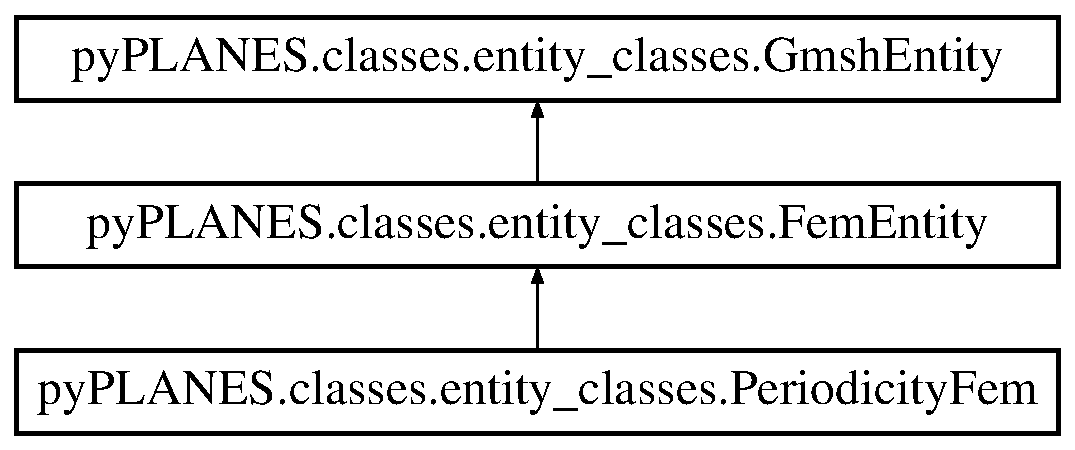
\includegraphics[height=3.000000cm]{classpy_p_l_a_n_e_s_1_1classes_1_1entity__classes_1_1_periodicity_fem}
\end{center}
\end{figure}
\subsection*{Public Member Functions}
\begin{DoxyCompactItemize}
\item 
\mbox{\Hypertarget{classpy_p_l_a_n_e_s_1_1classes_1_1entity__classes_1_1_periodicity_fem_af289f6608fc5fe2b43ef14606e169837}\label{classpy_p_l_a_n_e_s_1_1classes_1_1entity__classes_1_1_periodicity_fem_af289f6608fc5fe2b43ef14606e169837}} 
def {\bfseries \+\_\+\+\_\+init\+\_\+\+\_\+} (self, kwargs)
\item 
\mbox{\Hypertarget{classpy_p_l_a_n_e_s_1_1classes_1_1entity__classes_1_1_periodicity_fem_a13606781660f74bcf8be1985d78c2843}\label{classpy_p_l_a_n_e_s_1_1classes_1_1entity__classes_1_1_periodicity_fem_a13606781660f74bcf8be1985d78c2843}} 
def {\bfseries \+\_\+\+\_\+str\+\_\+\+\_\+} (self)
\end{DoxyCompactItemize}
\subsection*{Additional Inherited Members}


The documentation for this class was generated from the following file\+:\begin{DoxyCompactItemize}
\item 
py\+P\+L\+A\+N\+E\+S/classes/entity\+\_\+classes.\+py\end{DoxyCompactItemize}

\hypertarget{classpy_p_l_a_n_e_s_1_1fem_1_1elements_1_1reference__elements_1_1_plot_kt}{}\section{py\+P\+L\+A\+N\+E\+S.\+fem.\+elements.\+reference\+\_\+elements.\+Plot\+Kt Class Reference}
\label{classpy_p_l_a_n_e_s_1_1fem_1_1elements_1_1reference__elements_1_1_plot_kt}\index{py\+P\+L\+A\+N\+E\+S.\+fem.\+elements.\+reference\+\_\+elements.\+Plot\+Kt@{py\+P\+L\+A\+N\+E\+S.\+fem.\+elements.\+reference\+\_\+elements.\+Plot\+Kt}}
\subsection*{Public Member Functions}
\begin{DoxyCompactItemize}
\item 
\mbox{\Hypertarget{classpy_p_l_a_n_e_s_1_1fem_1_1elements_1_1reference__elements_1_1_plot_kt_a13ca5f9aeda97e45841bd77b454b58c4}\label{classpy_p_l_a_n_e_s_1_1fem_1_1elements_1_1reference__elements_1_1_plot_kt_a13ca5f9aeda97e45841bd77b454b58c4}} 
def {\bfseries \+\_\+\+\_\+init\+\_\+\+\_\+} (self, order=2)
\end{DoxyCompactItemize}
\subsection*{Public Attributes}
\begin{DoxyCompactItemize}
\item 
\mbox{\Hypertarget{classpy_p_l_a_n_e_s_1_1fem_1_1elements_1_1reference__elements_1_1_plot_kt_abc478f463a28762edb3e343e3fd0550d}\label{classpy_p_l_a_n_e_s_1_1fem_1_1elements_1_1reference__elements_1_1_plot_kt_abc478f463a28762edb3e343e3fd0550d}} 
{\bfseries order}
\item 
\mbox{\Hypertarget{classpy_p_l_a_n_e_s_1_1fem_1_1elements_1_1reference__elements_1_1_plot_kt_a360885cb9b9f72a6cd48cd97505694e8}\label{classpy_p_l_a_n_e_s_1_1fem_1_1elements_1_1reference__elements_1_1_plot_kt_a360885cb9b9f72a6cd48cd97505694e8}} 
{\bfseries nb\+\_\+v}
\item 
\mbox{\Hypertarget{classpy_p_l_a_n_e_s_1_1fem_1_1elements_1_1reference__elements_1_1_plot_kt_ad08640f7d41e5730576afde8b8f7cfdd}\label{classpy_p_l_a_n_e_s_1_1fem_1_1elements_1_1reference__elements_1_1_plot_kt_ad08640f7d41e5730576afde8b8f7cfdd}} 
{\bfseries nb\+\_\+e}
\item 
\mbox{\Hypertarget{classpy_p_l_a_n_e_s_1_1fem_1_1elements_1_1reference__elements_1_1_plot_kt_a79eba5c966144c50e9e739f2ddfe7ce0}\label{classpy_p_l_a_n_e_s_1_1fem_1_1elements_1_1reference__elements_1_1_plot_kt_a79eba5c966144c50e9e739f2ddfe7ce0}} 
{\bfseries nb\+\_\+f}
\item 
\mbox{\Hypertarget{classpy_p_l_a_n_e_s_1_1fem_1_1elements_1_1reference__elements_1_1_plot_kt_a1e38168497fc584eeff61944603890f3}\label{classpy_p_l_a_n_e_s_1_1fem_1_1elements_1_1reference__elements_1_1_plot_kt_a1e38168497fc584eeff61944603890f3}} 
{\bfseries nb\+\_\+\+SF}
\item 
\mbox{\Hypertarget{classpy_p_l_a_n_e_s_1_1fem_1_1elements_1_1reference__elements_1_1_plot_kt_ae5cb1bfc26a4878bb8807f44fdb438f3}\label{classpy_p_l_a_n_e_s_1_1fem_1_1elements_1_1reference__elements_1_1_plot_kt_ae5cb1bfc26a4878bb8807f44fdb438f3}} 
{\bfseries Phi}
\item 
\mbox{\Hypertarget{classpy_p_l_a_n_e_s_1_1fem_1_1elements_1_1reference__elements_1_1_plot_kt_a379e8b1f653c68fcc4ab9b41490954ab}\label{classpy_p_l_a_n_e_s_1_1fem_1_1elements_1_1reference__elements_1_1_plot_kt_a379e8b1f653c68fcc4ab9b41490954ab}} 
{\bfseries d\+Phi}
\end{DoxyCompactItemize}


The documentation for this class was generated from the following file\+:\begin{DoxyCompactItemize}
\item 
py\+P\+L\+A\+N\+E\+S/fem/elements/reference\+\_\+elements.\+py\end{DoxyCompactItemize}

\hypertarget{classpy_p_l_a_n_e_s_1_1gmsh_1_1write__geo__file_1_1_gmsh_1_1_point}{}\section{py\+P\+L\+A\+N\+E\+S.\+gmsh.\+write\+\_\+geo\+\_\+file.\+Gmsh.\+Point Class Reference}
\label{classpy_p_l_a_n_e_s_1_1gmsh_1_1write__geo__file_1_1_gmsh_1_1_point}\index{py\+P\+L\+A\+N\+E\+S.\+gmsh.\+write\+\_\+geo\+\_\+file.\+Gmsh.\+Point@{py\+P\+L\+A\+N\+E\+S.\+gmsh.\+write\+\_\+geo\+\_\+file.\+Gmsh.\+Point}}
\subsection*{Public Member Functions}
\begin{DoxyCompactItemize}
\item 
\mbox{\Hypertarget{classpy_p_l_a_n_e_s_1_1gmsh_1_1write__geo__file_1_1_gmsh_1_1_point_ac22b99f32ff7ce6a004ce7852a69da1d}\label{classpy_p_l_a_n_e_s_1_1gmsh_1_1write__geo__file_1_1_gmsh_1_1_point_ac22b99f32ff7ce6a004ce7852a69da1d}} 
def {\bfseries \+\_\+\+\_\+init\+\_\+\+\_\+} (self, f, tag, x, y, lc)
\end{DoxyCompactItemize}
\subsection*{Public Attributes}
\begin{DoxyCompactItemize}
\item 
\mbox{\Hypertarget{classpy_p_l_a_n_e_s_1_1gmsh_1_1write__geo__file_1_1_gmsh_1_1_point_a863f8ad65f9d28fdbd72edfcaadb4b52}\label{classpy_p_l_a_n_e_s_1_1gmsh_1_1write__geo__file_1_1_gmsh_1_1_point_a863f8ad65f9d28fdbd72edfcaadb4b52}} 
{\bfseries x}
\item 
\mbox{\Hypertarget{classpy_p_l_a_n_e_s_1_1gmsh_1_1write__geo__file_1_1_gmsh_1_1_point_a96956e2c0e3f88264312b6c2fffbc15a}\label{classpy_p_l_a_n_e_s_1_1gmsh_1_1write__geo__file_1_1_gmsh_1_1_point_a96956e2c0e3f88264312b6c2fffbc15a}} 
{\bfseries y}
\item 
\mbox{\Hypertarget{classpy_p_l_a_n_e_s_1_1gmsh_1_1write__geo__file_1_1_gmsh_1_1_point_a4c09e0d85ac5ffd631bb1a80b83b011a}\label{classpy_p_l_a_n_e_s_1_1gmsh_1_1write__geo__file_1_1_gmsh_1_1_point_a4c09e0d85ac5ffd631bb1a80b83b011a}} 
{\bfseries lc}
\item 
\mbox{\Hypertarget{classpy_p_l_a_n_e_s_1_1gmsh_1_1write__geo__file_1_1_gmsh_1_1_point_ae41f0755d91a10ab077fc7234a9477f8}\label{classpy_p_l_a_n_e_s_1_1gmsh_1_1write__geo__file_1_1_gmsh_1_1_point_ae41f0755d91a10ab077fc7234a9477f8}} 
{\bfseries tag}
\item 
\mbox{\Hypertarget{classpy_p_l_a_n_e_s_1_1gmsh_1_1write__geo__file_1_1_gmsh_1_1_point_ae54ce306525845b93a89dc1fa534e768}\label{classpy_p_l_a_n_e_s_1_1gmsh_1_1write__geo__file_1_1_gmsh_1_1_point_ae54ce306525845b93a89dc1fa534e768}} 
{\bfseries typ}
\end{DoxyCompactItemize}


The documentation for this class was generated from the following file\+:\begin{DoxyCompactItemize}
\item 
py\+P\+L\+A\+N\+E\+S/gmsh/write\+\_\+geo\+\_\+file.\+py\end{DoxyCompactItemize}

\hypertarget{classpy_p_l_a_n_e_s_1_1classes_1_1calculus_1_1_pw_calculus}{}\section{py\+P\+L\+A\+N\+E\+S.\+classes.\+calculus.\+Pw\+Calculus Class Reference}
\label{classpy_p_l_a_n_e_s_1_1classes_1_1calculus_1_1_pw_calculus}\index{py\+P\+L\+A\+N\+E\+S.\+classes.\+calculus.\+Pw\+Calculus@{py\+P\+L\+A\+N\+E\+S.\+classes.\+calculus.\+Pw\+Calculus}}
Inheritance diagram for py\+P\+L\+A\+N\+E\+S.\+classes.\+calculus.\+Pw\+Calculus\+:\begin{figure}[H]
\begin{center}
\leavevmode
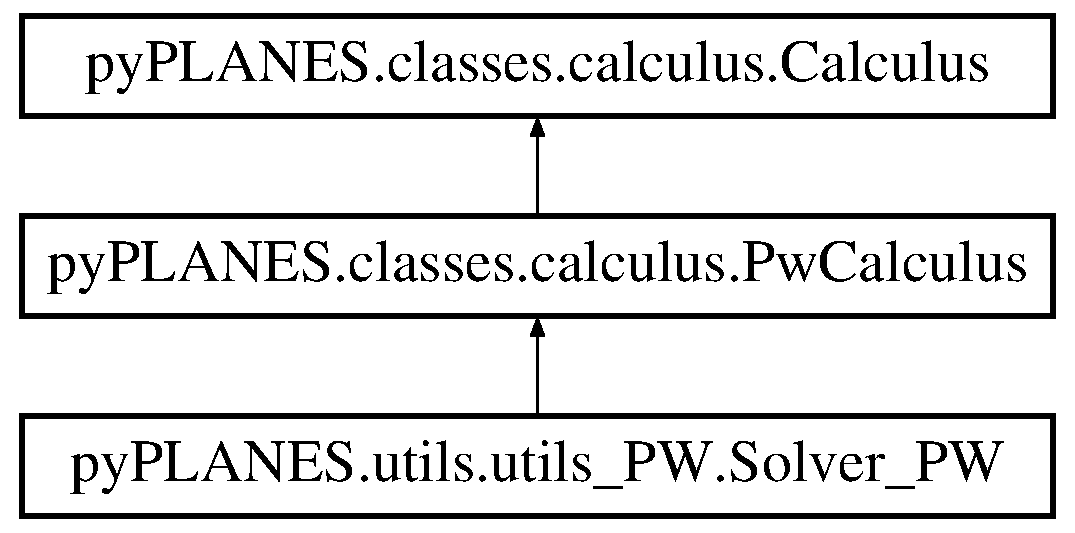
\includegraphics[height=3.000000cm]{classpy_p_l_a_n_e_s_1_1classes_1_1calculus_1_1_pw_calculus}
\end{center}
\end{figure}
\subsection*{Public Member Functions}
\begin{DoxyCompactItemize}
\item 
\mbox{\Hypertarget{classpy_p_l_a_n_e_s_1_1classes_1_1calculus_1_1_pw_calculus_a0adc73dcef5c022fb3b495e7e91850e0}\label{classpy_p_l_a_n_e_s_1_1classes_1_1calculus_1_1_pw_calculus_a0adc73dcef5c022fb3b495e7e91850e0}} 
def {\bfseries \+\_\+\+\_\+init\+\_\+\+\_\+} (self, kwargs)
\item 
\mbox{\Hypertarget{classpy_p_l_a_n_e_s_1_1classes_1_1calculus_1_1_pw_calculus_aefd14502b425dc36ec8395d71eff2343}\label{classpy_p_l_a_n_e_s_1_1classes_1_1calculus_1_1_pw_calculus_aefd14502b425dc36ec8395d71eff2343}} 
def {\bfseries update\+\_\+frequency} (self, f)
\end{DoxyCompactItemize}
\subsection*{Public Attributes}
\begin{DoxyCompactItemize}
\item 
\mbox{\Hypertarget{classpy_p_l_a_n_e_s_1_1classes_1_1calculus_1_1_pw_calculus_a96f5b385ba0181a3a30067966e9f3d26}\label{classpy_p_l_a_n_e_s_1_1classes_1_1calculus_1_1_pw_calculus_a96f5b385ba0181a3a30067966e9f3d26}} 
{\bfseries out\+\_\+file}
\item 
\mbox{\Hypertarget{classpy_p_l_a_n_e_s_1_1classes_1_1calculus_1_1_pw_calculus_ab3ad52ae651b9fdbd97298b6ac79b469}\label{classpy_p_l_a_n_e_s_1_1classes_1_1calculus_1_1_pw_calculus_ab3ad52ae651b9fdbd97298b6ac79b469}} 
{\bfseries info\+\_\+file}
\item 
\mbox{\Hypertarget{classpy_p_l_a_n_e_s_1_1classes_1_1calculus_1_1_pw_calculus_a97449d9b08d3423ae86638c5cd00a477}\label{classpy_p_l_a_n_e_s_1_1classes_1_1calculus_1_1_pw_calculus_a97449d9b08d3423ae86638c5cd00a477}} 
{\bfseries kx}
\item 
\mbox{\Hypertarget{classpy_p_l_a_n_e_s_1_1classes_1_1calculus_1_1_pw_calculus_a7de0a4be5a632e163bae9eef123f8781}\label{classpy_p_l_a_n_e_s_1_1classes_1_1calculus_1_1_pw_calculus_a7de0a4be5a632e163bae9eef123f8781}} 
{\bfseries ky}
\item 
\mbox{\Hypertarget{classpy_p_l_a_n_e_s_1_1classes_1_1calculus_1_1_pw_calculus_ab2584739426318c07540ac71e8a95a14}\label{classpy_p_l_a_n_e_s_1_1classes_1_1calculus_1_1_pw_calculus_ab2584739426318c07540ac71e8a95a14}} 
{\bfseries k}
\end{DoxyCompactItemize}


The documentation for this class was generated from the following file\+:\begin{DoxyCompactItemize}
\item 
py\+P\+L\+A\+N\+E\+S/classes/calculus.\+py\end{DoxyCompactItemize}

\hypertarget{classpy_p_l_a_n_e_s_1_1classes_1_1entity__classes_1_1_pw_fem}{}\section{py\+P\+L\+A\+N\+E\+S.\+classes.\+entity\+\_\+classes.\+Pw\+Fem Class Reference}
\label{classpy_p_l_a_n_e_s_1_1classes_1_1entity__classes_1_1_pw_fem}\index{py\+P\+L\+A\+N\+E\+S.\+classes.\+entity\+\_\+classes.\+Pw\+Fem@{py\+P\+L\+A\+N\+E\+S.\+classes.\+entity\+\_\+classes.\+Pw\+Fem}}
Inheritance diagram for py\+P\+L\+A\+N\+E\+S.\+classes.\+entity\+\_\+classes.\+Pw\+Fem\+:\begin{figure}[H]
\begin{center}
\leavevmode
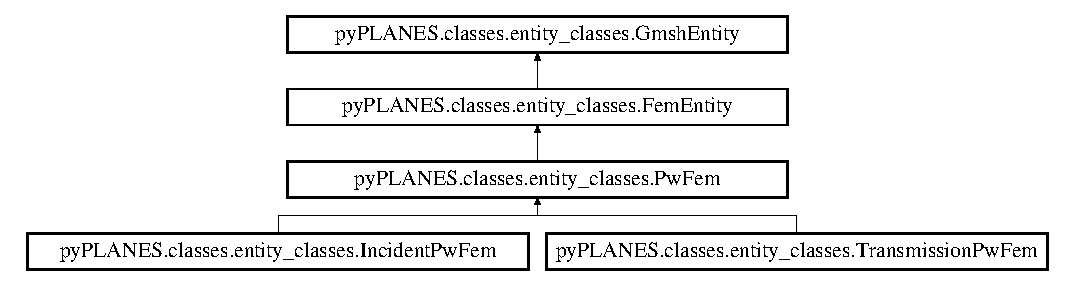
\includegraphics[height=3.393939cm]{classpy_p_l_a_n_e_s_1_1classes_1_1entity__classes_1_1_pw_fem}
\end{center}
\end{figure}
\subsection*{Public Member Functions}
\begin{DoxyCompactItemize}
\item 
\mbox{\Hypertarget{classpy_p_l_a_n_e_s_1_1classes_1_1entity__classes_1_1_pw_fem_a74e5ff97dc6fe487b32498fe214cf70d}\label{classpy_p_l_a_n_e_s_1_1classes_1_1entity__classes_1_1_pw_fem_a74e5ff97dc6fe487b32498fe214cf70d}} 
def {\bfseries \+\_\+\+\_\+init\+\_\+\+\_\+} (self, kwargs)
\item 
\mbox{\Hypertarget{classpy_p_l_a_n_e_s_1_1classes_1_1entity__classes_1_1_pw_fem_abcb4803ace9bd20f95b7c77ad3a76fbf}\label{classpy_p_l_a_n_e_s_1_1classes_1_1entity__classes_1_1_pw_fem_abcb4803ace9bd20f95b7c77ad3a76fbf}} 
def {\bfseries \+\_\+\+\_\+str\+\_\+\+\_\+} (self)
\item 
\mbox{\Hypertarget{classpy_p_l_a_n_e_s_1_1classes_1_1entity__classes_1_1_pw_fem_a075b70fe21e012b5b04f63f19afd241b}\label{classpy_p_l_a_n_e_s_1_1classes_1_1entity__classes_1_1_pw_fem_a075b70fe21e012b5b04f63f19afd241b}} 
def {\bfseries update\+\_\+frequency} (self, omega)
\item 
\mbox{\Hypertarget{classpy_p_l_a_n_e_s_1_1classes_1_1entity__classes_1_1_pw_fem_a26bd15bed479ab3485c5a8d0185382c2}\label{classpy_p_l_a_n_e_s_1_1classes_1_1entity__classes_1_1_pw_fem_a26bd15bed479ab3485c5a8d0185382c2}} 
def {\bfseries apply\+\_\+periodicity} (self, nb\+\_\+dof\+\_\+m, dof\+\_\+left, dof\+\_\+right, delta)
\end{DoxyCompactItemize}
\subsection*{Public Attributes}
\begin{DoxyCompactItemize}
\item 
\mbox{\Hypertarget{classpy_p_l_a_n_e_s_1_1classes_1_1entity__classes_1_1_pw_fem_a25b829eab7bf4b9bb06b9c87161a9101}\label{classpy_p_l_a_n_e_s_1_1classes_1_1entity__classes_1_1_pw_fem_a25b829eab7bf4b9bb06b9c87161a9101}} 
{\bfseries A\+\_\+v}
\item 
\mbox{\Hypertarget{classpy_p_l_a_n_e_s_1_1classes_1_1entity__classes_1_1_pw_fem_aaeeebf0c647ee5b999ca542a94ab5f9b}\label{classpy_p_l_a_n_e_s_1_1classes_1_1entity__classes_1_1_pw_fem_aaeeebf0c647ee5b999ca542a94ab5f9b}} 
{\bfseries F\+\_\+v}
\item 
\mbox{\Hypertarget{classpy_p_l_a_n_e_s_1_1classes_1_1entity__classes_1_1_pw_fem_a0daa53e5a323f11f2ebb6bf66fd5bb0e}\label{classpy_p_l_a_n_e_s_1_1classes_1_1entity__classes_1_1_pw_fem_a0daa53e5a323f11f2ebb6bf66fd5bb0e}} 
{\bfseries dofs}
\item 
\mbox{\Hypertarget{classpy_p_l_a_n_e_s_1_1classes_1_1entity__classes_1_1_pw_fem_a11f8dbcf56c7eb10ce6b65ac1948bad5}\label{classpy_p_l_a_n_e_s_1_1classes_1_1entity__classes_1_1_pw_fem_a11f8dbcf56c7eb10ce6b65ac1948bad5}} 
{\bfseries theta\+\_\+d}
\item 
\mbox{\Hypertarget{classpy_p_l_a_n_e_s_1_1classes_1_1entity__classes_1_1_pw_fem_a6ce15d3e1e6cb9b9907a174fccf252c1}\label{classpy_p_l_a_n_e_s_1_1classes_1_1entity__classes_1_1_pw_fem_a6ce15d3e1e6cb9b9907a174fccf252c1}} 
{\bfseries ky}
\item 
\mbox{\Hypertarget{classpy_p_l_a_n_e_s_1_1classes_1_1entity__classes_1_1_pw_fem_a2ef4ddb156ed0201e1e7a49b8c5f8bd8}\label{classpy_p_l_a_n_e_s_1_1classes_1_1entity__classes_1_1_pw_fem_a2ef4ddb156ed0201e1e7a49b8c5f8bd8}} 
{\bfseries phi\+\_\+v}
\item 
\mbox{\Hypertarget{classpy_p_l_a_n_e_s_1_1classes_1_1entity__classes_1_1_pw_fem_a7318d34e72b51873da68bbb10d8defe2}\label{classpy_p_l_a_n_e_s_1_1classes_1_1entity__classes_1_1_pw_fem_a7318d34e72b51873da68bbb10d8defe2}} 
{\bfseries nb\+\_\+dofs}
\item 
\mbox{\Hypertarget{classpy_p_l_a_n_e_s_1_1classes_1_1entity__classes_1_1_pw_fem_a47bbac1d42c22c54df0d0a4afed69f7d}\label{classpy_p_l_a_n_e_s_1_1classes_1_1entity__classes_1_1_pw_fem_a47bbac1d42c22c54df0d0a4afed69f7d}} 
{\bfseries Omega\+\_\+orth}
\item 
\mbox{\Hypertarget{classpy_p_l_a_n_e_s_1_1classes_1_1entity__classes_1_1_pw_fem_ac103cd80a883cf95d51353e51b05bfa3}\label{classpy_p_l_a_n_e_s_1_1classes_1_1entity__classes_1_1_pw_fem_ac103cd80a883cf95d51353e51b05bfa3}} 
{\bfseries ny}
\item 
\mbox{\Hypertarget{classpy_p_l_a_n_e_s_1_1classes_1_1entity__classes_1_1_pw_fem_a86408b39d1c03be2c3db6b00d273fa18}\label{classpy_p_l_a_n_e_s_1_1classes_1_1entity__classes_1_1_pw_fem_a86408b39d1c03be2c3db6b00d273fa18}} 
{\bfseries ml}
\item 
\mbox{\Hypertarget{classpy_p_l_a_n_e_s_1_1classes_1_1entity__classes_1_1_pw_fem_abc22b938ff29b63f895489cb876595c3}\label{classpy_p_l_a_n_e_s_1_1classes_1_1entity__classes_1_1_pw_fem_abc22b938ff29b63f895489cb876595c3}} 
{\bfseries nb\+\_\+waves}
\item 
\mbox{\Hypertarget{classpy_p_l_a_n_e_s_1_1classes_1_1entity__classes_1_1_pw_fem_a2ad23c4a150e07fac41af577bdd10315}\label{classpy_p_l_a_n_e_s_1_1classes_1_1entity__classes_1_1_pw_fem_a2ad23c4a150e07fac41af577bdd10315}} 
{\bfseries kx}
\item 
\mbox{\Hypertarget{classpy_p_l_a_n_e_s_1_1classes_1_1entity__classes_1_1_pw_fem_a703dc5b433d331858f5516c980334fe9}\label{classpy_p_l_a_n_e_s_1_1classes_1_1entity__classes_1_1_pw_fem_a703dc5b433d331858f5516c980334fe9}} 
{\bfseries phi\+\_\+i}
\item 
\mbox{\Hypertarget{classpy_p_l_a_n_e_s_1_1classes_1_1entity__classes_1_1_pw_fem_a6f8596fe571dc0e3702ca5af011fba1b}\label{classpy_p_l_a_n_e_s_1_1classes_1_1entity__classes_1_1_pw_fem_a6f8596fe571dc0e3702ca5af011fba1b}} 
{\bfseries phi}
\end{DoxyCompactItemize}


The documentation for this class was generated from the following file\+:\begin{DoxyCompactItemize}
\item 
py\+P\+L\+A\+N\+E\+S/classes/entity\+\_\+classes.\+py\end{DoxyCompactItemize}

\hypertarget{classpy_p_l_a_n_e_s_1_1classes_1_1entity__classes_1_1_rigid_wall_fem}{}\section{py\+P\+L\+A\+N\+E\+S.\+classes.\+entity\+\_\+classes.\+Rigid\+Wall\+Fem Class Reference}
\label{classpy_p_l_a_n_e_s_1_1classes_1_1entity__classes_1_1_rigid_wall_fem}\index{py\+P\+L\+A\+N\+E\+S.\+classes.\+entity\+\_\+classes.\+Rigid\+Wall\+Fem@{py\+P\+L\+A\+N\+E\+S.\+classes.\+entity\+\_\+classes.\+Rigid\+Wall\+Fem}}
Inheritance diagram for py\+P\+L\+A\+N\+E\+S.\+classes.\+entity\+\_\+classes.\+Rigid\+Wall\+Fem\+:\begin{figure}[H]
\begin{center}
\leavevmode
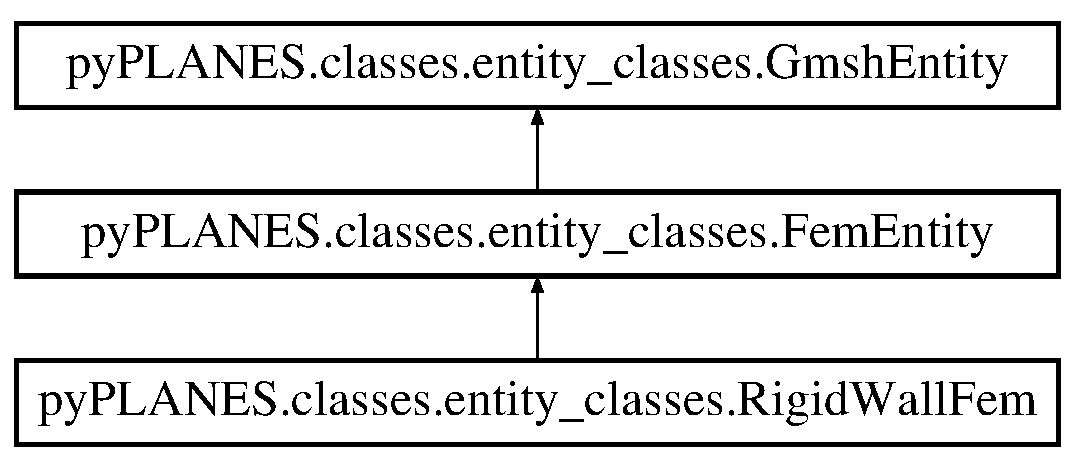
\includegraphics[height=3.000000cm]{classpy_p_l_a_n_e_s_1_1classes_1_1entity__classes_1_1_rigid_wall_fem}
\end{center}
\end{figure}
\subsection*{Public Member Functions}
\begin{DoxyCompactItemize}
\item 
\mbox{\Hypertarget{classpy_p_l_a_n_e_s_1_1classes_1_1entity__classes_1_1_rigid_wall_fem_a72f1e21db6dcd43a75ac948bcfcd15b2}\label{classpy_p_l_a_n_e_s_1_1classes_1_1entity__classes_1_1_rigid_wall_fem_a72f1e21db6dcd43a75ac948bcfcd15b2}} 
def {\bfseries \+\_\+\+\_\+init\+\_\+\+\_\+} (self, kwargs)
\item 
\mbox{\Hypertarget{classpy_p_l_a_n_e_s_1_1classes_1_1entity__classes_1_1_rigid_wall_fem_a3250eded3fc49e0fc5ca53d065cbd937}\label{classpy_p_l_a_n_e_s_1_1classes_1_1entity__classes_1_1_rigid_wall_fem_a3250eded3fc49e0fc5ca53d065cbd937}} 
def {\bfseries \+\_\+\+\_\+str\+\_\+\+\_\+} (self)
\end{DoxyCompactItemize}
\subsection*{Additional Inherited Members}


The documentation for this class was generated from the following file\+:\begin{DoxyCompactItemize}
\item 
py\+P\+L\+A\+N\+E\+S/classes/entity\+\_\+classes.\+py\end{DoxyCompactItemize}

\hypertarget{classpy_p_l_a_n_e_s_1_1utils_1_1utils___p_w_1_1_solver___p_w}{}\section{py\+P\+L\+A\+N\+E\+S.\+utils.\+utils\+\_\+\+P\+W.\+Solver\+\_\+\+PW Class Reference}
\label{classpy_p_l_a_n_e_s_1_1utils_1_1utils___p_w_1_1_solver___p_w}\index{py\+P\+L\+A\+N\+E\+S.\+utils.\+utils\+\_\+\+P\+W.\+Solver\+\_\+\+PW@{py\+P\+L\+A\+N\+E\+S.\+utils.\+utils\+\_\+\+P\+W.\+Solver\+\_\+\+PW}}
Inheritance diagram for py\+P\+L\+A\+N\+E\+S.\+utils.\+utils\+\_\+\+P\+W.\+Solver\+\_\+\+PW\+:\begin{figure}[H]
\begin{center}
\leavevmode
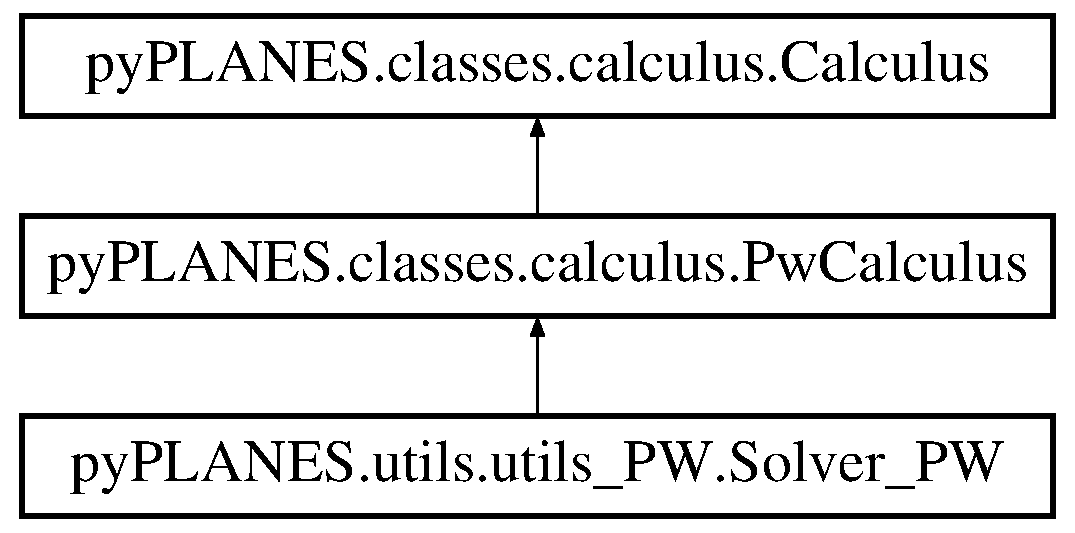
\includegraphics[height=3.000000cm]{classpy_p_l_a_n_e_s_1_1utils_1_1utils___p_w_1_1_solver___p_w}
\end{center}
\end{figure}
\subsection*{Public Member Functions}
\begin{DoxyCompactItemize}
\item 
\mbox{\Hypertarget{classpy_p_l_a_n_e_s_1_1utils_1_1utils___p_w_1_1_solver___p_w_add21272a7df71502e1368983e28f5d81}\label{classpy_p_l_a_n_e_s_1_1utils_1_1utils___p_w_1_1_solver___p_w_add21272a7df71502e1368983e28f5d81}} 
def {\bfseries \+\_\+\+\_\+init\+\_\+\+\_\+} (self, kwargs)
\item 
\mbox{\Hypertarget{classpy_p_l_a_n_e_s_1_1utils_1_1utils___p_w_1_1_solver___p_w_aafa29063579a5ddcad811066462d0032}\label{classpy_p_l_a_n_e_s_1_1utils_1_1utils___p_w_1_1_solver___p_w_aafa29063579a5ddcad811066462d0032}} 
def {\bfseries write\+\_\+out\+\_\+files} (self, out)
\item 
\mbox{\Hypertarget{classpy_p_l_a_n_e_s_1_1utils_1_1utils___p_w_1_1_solver___p_w_a4550f2968b6fa45ab7f9a4052c2aa05a}\label{classpy_p_l_a_n_e_s_1_1utils_1_1utils___p_w_1_1_solver___p_w_a4550f2968b6fa45ab7f9a4052c2aa05a}} 
def {\bfseries resolution} (self, theta\+\_\+d)
\item 
\mbox{\Hypertarget{classpy_p_l_a_n_e_s_1_1utils_1_1utils___p_w_1_1_solver___p_w_ab74b920da54e68243dddf6dee74da8a4}\label{classpy_p_l_a_n_e_s_1_1utils_1_1utils___p_w_1_1_solver___p_w_ab74b920da54e68243dddf6dee74da8a4}} 
def {\bfseries solve} (self, f, theta\+\_\+d)
\item 
\mbox{\Hypertarget{classpy_p_l_a_n_e_s_1_1utils_1_1utils___p_w_1_1_solver___p_w_aa8a2580d7f6bd12ed9fbad4703c576eb}\label{classpy_p_l_a_n_e_s_1_1utils_1_1utils___p_w_1_1_solver___p_w_aa8a2580d7f6bd12ed9fbad4703c576eb}} 
def {\bfseries interface\+\_\+fluid\+\_\+fluid} (self, ieq, iinter, L, d, M)
\item 
\mbox{\Hypertarget{classpy_p_l_a_n_e_s_1_1utils_1_1utils___p_w_1_1_solver___p_w_adba422cfae632b76eacd8cd7927a5797}\label{classpy_p_l_a_n_e_s_1_1utils_1_1utils___p_w_1_1_solver___p_w_adba422cfae632b76eacd8cd7927a5797}} 
def {\bfseries interface\+\_\+fluid\+\_\+rigid} (self, M, ieq, L, d)
\item 
\mbox{\Hypertarget{classpy_p_l_a_n_e_s_1_1utils_1_1utils___p_w_1_1_solver___p_w_a1f56642fc51ae6503b67514f360fee15}\label{classpy_p_l_a_n_e_s_1_1utils_1_1utils___p_w_1_1_solver___p_w_a1f56642fc51ae6503b67514f360fee15}} 
def {\bfseries semi\+\_\+infinite\+\_\+medium} (self, M, ieq, L, d)
\item 
\mbox{\Hypertarget{classpy_p_l_a_n_e_s_1_1utils_1_1utils___p_w_1_1_solver___p_w_a34ef8f9c70991762cc275531360c283a}\label{classpy_p_l_a_n_e_s_1_1utils_1_1utils___p_w_1_1_solver___p_w_a34ef8f9c70991762cc275531360c283a}} 
def {\bfseries interface\+\_\+pem\+\_\+pem} (self, ieq, iinter, L, d, M)
\item 
\mbox{\Hypertarget{classpy_p_l_a_n_e_s_1_1utils_1_1utils___p_w_1_1_solver___p_w_a6b13710cf516d74ca1d7f31964c1b60a}\label{classpy_p_l_a_n_e_s_1_1utils_1_1utils___p_w_1_1_solver___p_w_a6b13710cf516d74ca1d7f31964c1b60a}} 
def {\bfseries interface\+\_\+fluid\+\_\+pem} (self, ieq, iinter, L, d, M)
\item 
\mbox{\Hypertarget{classpy_p_l_a_n_e_s_1_1utils_1_1utils___p_w_1_1_solver___p_w_ae42fe83ae3b396b3b8ae9c538ae28e7d}\label{classpy_p_l_a_n_e_s_1_1utils_1_1utils___p_w_1_1_solver___p_w_ae42fe83ae3b396b3b8ae9c538ae28e7d}} 
def {\bfseries interface\+\_\+elastic\+\_\+pem} (self, ieq, iinter, L, d, M)
\item 
\mbox{\Hypertarget{classpy_p_l_a_n_e_s_1_1utils_1_1utils___p_w_1_1_solver___p_w_a5e8fedc74b29e26aca67bcc1e3831fc8}\label{classpy_p_l_a_n_e_s_1_1utils_1_1utils___p_w_1_1_solver___p_w_a5e8fedc74b29e26aca67bcc1e3831fc8}} 
def {\bfseries interface\+\_\+pem\+\_\+elastic} (self, ieq, iinter, L, d, M)
\item 
\mbox{\Hypertarget{classpy_p_l_a_n_e_s_1_1utils_1_1utils___p_w_1_1_solver___p_w_acb3d52f844c88f66eac0e5b43e99f1c3}\label{classpy_p_l_a_n_e_s_1_1utils_1_1utils___p_w_1_1_solver___p_w_acb3d52f844c88f66eac0e5b43e99f1c3}} 
def {\bfseries interface\+\_\+elastic\+\_\+elastic} (self, ieq, iinter, L, d, M)
\item 
\mbox{\Hypertarget{classpy_p_l_a_n_e_s_1_1utils_1_1utils___p_w_1_1_solver___p_w_ad5dd9b68b4bd1f50a85b53632ca2db5e}\label{classpy_p_l_a_n_e_s_1_1utils_1_1utils___p_w_1_1_solver___p_w_ad5dd9b68b4bd1f50a85b53632ca2db5e}} 
def {\bfseries interface\+\_\+fluid\+\_\+elastic} (self, ieq, iinter, L, d, M)
\item 
\mbox{\Hypertarget{classpy_p_l_a_n_e_s_1_1utils_1_1utils___p_w_1_1_solver___p_w_acb36b625deb7a6c0f7527240c4cd12e7}\label{classpy_p_l_a_n_e_s_1_1utils_1_1utils___p_w_1_1_solver___p_w_acb36b625deb7a6c0f7527240c4cd12e7}} 
def {\bfseries interface\+\_\+pem\+\_\+fluid} (self, ieq, iinter, L, d, M)
\item 
\mbox{\Hypertarget{classpy_p_l_a_n_e_s_1_1utils_1_1utils___p_w_1_1_solver___p_w_ab4727334240be500563b99f632326296}\label{classpy_p_l_a_n_e_s_1_1utils_1_1utils___p_w_1_1_solver___p_w_ab4727334240be500563b99f632326296}} 
def {\bfseries interface\+\_\+elastic\+\_\+fluid} (self, ieq, iinter, L, d, M)
\item 
\mbox{\Hypertarget{classpy_p_l_a_n_e_s_1_1utils_1_1utils___p_w_1_1_solver___p_w_af2603f7c6e8e93e7e0bf14f684ffa3b0}\label{classpy_p_l_a_n_e_s_1_1utils_1_1utils___p_w_1_1_solver___p_w_af2603f7c6e8e93e7e0bf14f684ffa3b0}} 
def {\bfseries interface\+\_\+elastic\+\_\+rigid} (self, M, ieq, L, d)
\item 
\mbox{\Hypertarget{classpy_p_l_a_n_e_s_1_1utils_1_1utils___p_w_1_1_solver___p_w_a03863718254b21889be4f8e4ab2ce5ee}\label{classpy_p_l_a_n_e_s_1_1utils_1_1utils___p_w_1_1_solver___p_w_a03863718254b21889be4f8e4ab2ce5ee}} 
def {\bfseries interface\+\_\+pem\+\_\+rigid} (self, M, ieq, L, d)
\item 
\mbox{\Hypertarget{classpy_p_l_a_n_e_s_1_1utils_1_1utils___p_w_1_1_solver___p_w_ac2be15b456dacc16909d0527a8c23e04}\label{classpy_p_l_a_n_e_s_1_1utils_1_1utils___p_w_1_1_solver___p_w_ac2be15b456dacc16909d0527a8c23e04}} 
def {\bfseries plot\+\_\+sol\+\_\+\+PW} (self, X, dofs)
\end{DoxyCompactItemize}
\subsection*{Public Attributes}
\begin{DoxyCompactItemize}
\item 
\mbox{\Hypertarget{classpy_p_l_a_n_e_s_1_1utils_1_1utils___p_w_1_1_solver___p_w_ab26a1a4e82049dbd195375b0f79e40e5}\label{classpy_p_l_a_n_e_s_1_1utils_1_1utils___p_w_1_1_solver___p_w_ab26a1a4e82049dbd195375b0f79e40e5}} 
{\bfseries layers}
\item 
\mbox{\Hypertarget{classpy_p_l_a_n_e_s_1_1utils_1_1utils___p_w_1_1_solver___p_w_a9b8719bba7a36ab3c27ca64f3cc72d30}\label{classpy_p_l_a_n_e_s_1_1utils_1_1utils___p_w_1_1_solver___p_w_a9b8719bba7a36ab3c27ca64f3cc72d30}} 
{\bfseries backing}
\item 
\mbox{\Hypertarget{classpy_p_l_a_n_e_s_1_1utils_1_1utils___p_w_1_1_solver___p_w_a51d6873336355d7bb718058b571c4cff}\label{classpy_p_l_a_n_e_s_1_1utils_1_1utils___p_w_1_1_solver___p_w_a51d6873336355d7bb718058b571c4cff}} 
{\bfseries k}
\item 
\mbox{\Hypertarget{classpy_p_l_a_n_e_s_1_1utils_1_1utils___p_w_1_1_solver___p_w_a50fd0129383834bb4e94637eafc8e5ba}\label{classpy_p_l_a_n_e_s_1_1utils_1_1utils___p_w_1_1_solver___p_w_a50fd0129383834bb4e94637eafc8e5ba}} 
{\bfseries shift\+\_\+plot}
\item 
\mbox{\Hypertarget{classpy_p_l_a_n_e_s_1_1utils_1_1utils___p_w_1_1_solver___p_w_a9f138ad814bb126c73e72b5598ab02a3}\label{classpy_p_l_a_n_e_s_1_1utils_1_1utils___p_w_1_1_solver___p_w_a9f138ad814bb126c73e72b5598ab02a3}} 
{\bfseries plot}
\item 
\mbox{\Hypertarget{classpy_p_l_a_n_e_s_1_1utils_1_1utils___p_w_1_1_solver___p_w_a2178308183f5de0f1eb5f43adcf71961}\label{classpy_p_l_a_n_e_s_1_1utils_1_1utils___p_w_1_1_solver___p_w_a2178308183f5de0f1eb5f43adcf71961}} 
{\bfseries result}
\item 
\mbox{\Hypertarget{classpy_p_l_a_n_e_s_1_1utils_1_1utils___p_w_1_1_solver___p_w_aa449d46edc58cb8ab584265ad6fc42ed}\label{classpy_p_l_a_n_e_s_1_1utils_1_1utils___p_w_1_1_solver___p_w_aa449d46edc58cb8ab584265ad6fc42ed}} 
{\bfseries outfiles\+\_\+directory}
\end{DoxyCompactItemize}


The documentation for this class was generated from the following file\+:\begin{DoxyCompactItemize}
\item 
py\+P\+L\+A\+N\+E\+S/utils/utils\+\_\+\+P\+W.\+py\end{DoxyCompactItemize}

\hypertarget{classpy_p_l_a_n_e_s_1_1gmsh_1_1write__geo__file_1_1_gmsh_1_1_surface}{}\section{py\+P\+L\+A\+N\+E\+S.\+gmsh.\+write\+\_\+geo\+\_\+file.\+Gmsh.\+Surface Class Reference}
\label{classpy_p_l_a_n_e_s_1_1gmsh_1_1write__geo__file_1_1_gmsh_1_1_surface}\index{py\+P\+L\+A\+N\+E\+S.\+gmsh.\+write\+\_\+geo\+\_\+file.\+Gmsh.\+Surface@{py\+P\+L\+A\+N\+E\+S.\+gmsh.\+write\+\_\+geo\+\_\+file.\+Gmsh.\+Surface}}
\subsection*{Public Member Functions}
\begin{DoxyCompactItemize}
\item 
\mbox{\Hypertarget{classpy_p_l_a_n_e_s_1_1gmsh_1_1write__geo__file_1_1_gmsh_1_1_surface_ad4edc24353b60a511eb5ea716d5e0e8f}\label{classpy_p_l_a_n_e_s_1_1gmsh_1_1write__geo__file_1_1_gmsh_1_1_surface_ad4edc24353b60a511eb5ea716d5e0e8f}} 
def {\bfseries \+\_\+\+\_\+init\+\_\+\+\_\+} (self, f, tag, ll)
\end{DoxyCompactItemize}
\subsection*{Public Attributes}
\begin{DoxyCompactItemize}
\item 
\mbox{\Hypertarget{classpy_p_l_a_n_e_s_1_1gmsh_1_1write__geo__file_1_1_gmsh_1_1_surface_a737f308b622e686ad3eb5946426996a4}\label{classpy_p_l_a_n_e_s_1_1gmsh_1_1write__geo__file_1_1_gmsh_1_1_surface_a737f308b622e686ad3eb5946426996a4}} 
{\bfseries ll}
\item 
\mbox{\Hypertarget{classpy_p_l_a_n_e_s_1_1gmsh_1_1write__geo__file_1_1_gmsh_1_1_surface_a30121a4663da81cf268d92b15420fc00}\label{classpy_p_l_a_n_e_s_1_1gmsh_1_1write__geo__file_1_1_gmsh_1_1_surface_a30121a4663da81cf268d92b15420fc00}} 
{\bfseries tag}
\item 
\mbox{\Hypertarget{classpy_p_l_a_n_e_s_1_1gmsh_1_1write__geo__file_1_1_gmsh_1_1_surface_a24c08ac3516de66fe3fd053021ed91dd}\label{classpy_p_l_a_n_e_s_1_1gmsh_1_1write__geo__file_1_1_gmsh_1_1_surface_a24c08ac3516de66fe3fd053021ed91dd}} 
{\bfseries typ}
\end{DoxyCompactItemize}


The documentation for this class was generated from the following file\+:\begin{DoxyCompactItemize}
\item 
py\+P\+L\+A\+N\+E\+S/gmsh/write\+\_\+geo\+\_\+file.\+py\end{DoxyCompactItemize}

\hypertarget{classpy_p_l_a_n_e_s_1_1classes_1_1entity__classes_1_1_transmission_pw_fem}{}\section{py\+P\+L\+A\+N\+E\+S.\+classes.\+entity\+\_\+classes.\+Transmission\+Pw\+Fem Class Reference}
\label{classpy_p_l_a_n_e_s_1_1classes_1_1entity__classes_1_1_transmission_pw_fem}\index{py\+P\+L\+A\+N\+E\+S.\+classes.\+entity\+\_\+classes.\+Transmission\+Pw\+Fem@{py\+P\+L\+A\+N\+E\+S.\+classes.\+entity\+\_\+classes.\+Transmission\+Pw\+Fem}}
Inheritance diagram for py\+P\+L\+A\+N\+E\+S.\+classes.\+entity\+\_\+classes.\+Transmission\+Pw\+Fem\+:\begin{figure}[H]
\begin{center}
\leavevmode
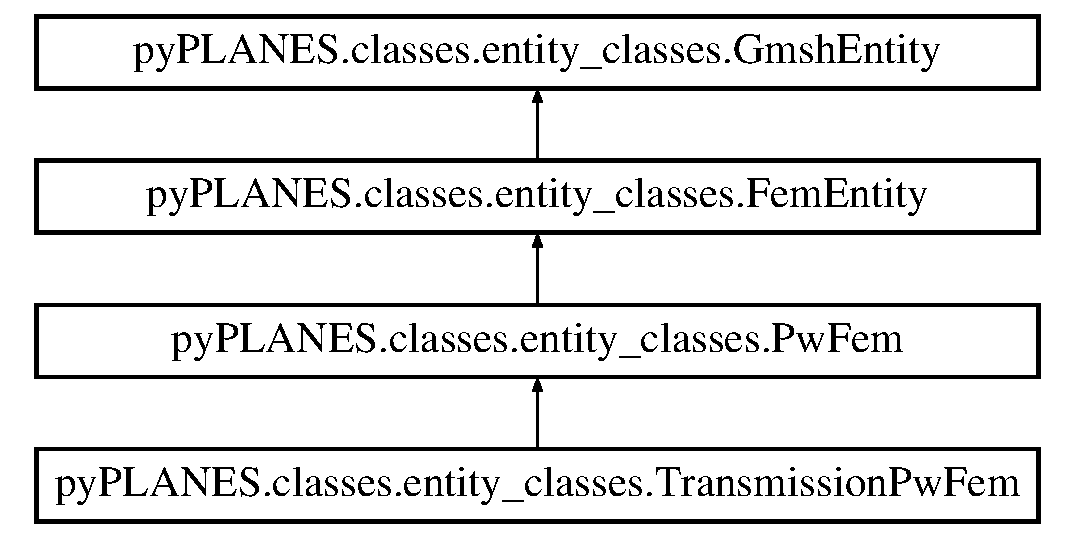
\includegraphics[height=4.000000cm]{classpy_p_l_a_n_e_s_1_1classes_1_1entity__classes_1_1_transmission_pw_fem}
\end{center}
\end{figure}
\subsection*{Public Member Functions}
\begin{DoxyCompactItemize}
\item 
\mbox{\Hypertarget{classpy_p_l_a_n_e_s_1_1classes_1_1entity__classes_1_1_transmission_pw_fem_a485973bec5065400d5cc887e8c7e637e}\label{classpy_p_l_a_n_e_s_1_1classes_1_1entity__classes_1_1_transmission_pw_fem_a485973bec5065400d5cc887e8c7e637e}} 
def {\bfseries \+\_\+\+\_\+init\+\_\+\+\_\+} (self, kwargs)
\item 
\mbox{\Hypertarget{classpy_p_l_a_n_e_s_1_1classes_1_1entity__classes_1_1_transmission_pw_fem_a19cac437006cc595b32049628d72be4d}\label{classpy_p_l_a_n_e_s_1_1classes_1_1entity__classes_1_1_transmission_pw_fem_a19cac437006cc595b32049628d72be4d}} 
def {\bfseries \+\_\+\+\_\+str\+\_\+\+\_\+} (self)
\item 
\mbox{\Hypertarget{classpy_p_l_a_n_e_s_1_1classes_1_1entity__classes_1_1_transmission_pw_fem_a79b248456f6d23dd99a1e7cb7ec7a97f}\label{classpy_p_l_a_n_e_s_1_1classes_1_1entity__classes_1_1_transmission_pw_fem_a79b248456f6d23dd99a1e7cb7ec7a97f}} 
def {\bfseries get\+\_\+wave\+\_\+dofs} (self, \+\_\+l)
\item 
\mbox{\Hypertarget{classpy_p_l_a_n_e_s_1_1classes_1_1entity__classes_1_1_transmission_pw_fem_abd1fa8c18c55fa451c8a14afb3beaf34}\label{classpy_p_l_a_n_e_s_1_1classes_1_1entity__classes_1_1_transmission_pw_fem_abd1fa8c18c55fa451c8a14afb3beaf34}} 
def {\bfseries get\+\_\+tau\+\_\+eta} (self, kx, ky, om)
\item 
\mbox{\Hypertarget{classpy_p_l_a_n_e_s_1_1classes_1_1entity__classes_1_1_transmission_pw_fem_aaf0e7d7269bfadc227378e868ab26f3c}\label{classpy_p_l_a_n_e_s_1_1classes_1_1entity__classes_1_1_transmission_pw_fem_aaf0e7d7269bfadc227378e868ab26f3c}} 
def {\bfseries create\+\_\+dynamical\+\_\+matrices} (self, omega, n\+\_\+m)
\end{DoxyCompactItemize}
\subsection*{Public Attributes}
\begin{DoxyCompactItemize}
\item 
\mbox{\Hypertarget{classpy_p_l_a_n_e_s_1_1classes_1_1entity__classes_1_1_transmission_pw_fem_aaadc0d06ae044fd86d67ed193650c12a}\label{classpy_p_l_a_n_e_s_1_1classes_1_1entity__classes_1_1_transmission_pw_fem_aaadc0d06ae044fd86d67ed193650c12a}} 
{\bfseries ny}
\item 
\mbox{\Hypertarget{classpy_p_l_a_n_e_s_1_1classes_1_1entity__classes_1_1_transmission_pw_fem_a2ed0cc1245d69c4683b5aecbb24c0677}\label{classpy_p_l_a_n_e_s_1_1classes_1_1entity__classes_1_1_transmission_pw_fem_a2ed0cc1245d69c4683b5aecbb24c0677}} 
{\bfseries eta\+\_\+\+TM}
\item 
\mbox{\Hypertarget{classpy_p_l_a_n_e_s_1_1classes_1_1entity__classes_1_1_transmission_pw_fem_a3df7dc99a164d0bb8639ab27cc004b79}\label{classpy_p_l_a_n_e_s_1_1classes_1_1entity__classes_1_1_transmission_pw_fem_a3df7dc99a164d0bb8639ab27cc004b79}} 
{\bfseries typ}
\item 
\mbox{\Hypertarget{classpy_p_l_a_n_e_s_1_1classes_1_1entity__classes_1_1_transmission_pw_fem_af870424308c699a4b9294aeb824e3b09}\label{classpy_p_l_a_n_e_s_1_1classes_1_1entity__classes_1_1_transmission_pw_fem_af870424308c699a4b9294aeb824e3b09}} 
{\bfseries phi\+\_\+v}
\end{DoxyCompactItemize}


The documentation for this class was generated from the following file\+:\begin{DoxyCompactItemize}
\item 
py\+P\+L\+A\+N\+E\+S/classes/entity\+\_\+classes.\+py\end{DoxyCompactItemize}

\hypertarget{classpy_p_l_a_n_e_s_1_1classes_1_1fem__classes_1_1_vertex}{}\section{py\+P\+L\+A\+N\+E\+S.\+classes.\+fem\+\_\+classes.\+Vertex Class Reference}
\label{classpy_p_l_a_n_e_s_1_1classes_1_1fem__classes_1_1_vertex}\index{py\+P\+L\+A\+N\+E\+S.\+classes.\+fem\+\_\+classes.\+Vertex@{py\+P\+L\+A\+N\+E\+S.\+classes.\+fem\+\_\+classes.\+Vertex}}
\subsection*{Public Member Functions}
\begin{DoxyCompactItemize}
\item 
\mbox{\Hypertarget{classpy_p_l_a_n_e_s_1_1classes_1_1fem__classes_1_1_vertex_ab3a5735bafaa07a1d4169ff36c1ca877}\label{classpy_p_l_a_n_e_s_1_1classes_1_1fem__classes_1_1_vertex_ab3a5735bafaa07a1d4169ff36c1ca877}} 
def {\bfseries \+\_\+\+\_\+init\+\_\+\+\_\+} (self, coord, tag)
\item 
\mbox{\Hypertarget{classpy_p_l_a_n_e_s_1_1classes_1_1fem__classes_1_1_vertex_a55ca9ffcaa29bd1b4fb604153719d91e}\label{classpy_p_l_a_n_e_s_1_1classes_1_1fem__classes_1_1_vertex_a55ca9ffcaa29bd1b4fb604153719d91e}} 
def {\bfseries \+\_\+\+\_\+str\+\_\+\+\_\+} (self)
\end{DoxyCompactItemize}
\subsection*{Public Attributes}
\begin{DoxyCompactItemize}
\item 
\mbox{\Hypertarget{classpy_p_l_a_n_e_s_1_1classes_1_1fem__classes_1_1_vertex_a96e1a6d9158707e4af8fadfa8f406b0c}\label{classpy_p_l_a_n_e_s_1_1classes_1_1fem__classes_1_1_vertex_a96e1a6d9158707e4af8fadfa8f406b0c}} 
{\bfseries coord}
\item 
\mbox{\Hypertarget{classpy_p_l_a_n_e_s_1_1classes_1_1fem__classes_1_1_vertex_ac884dc4c536579a42d8e19b205ad37fc}\label{classpy_p_l_a_n_e_s_1_1classes_1_1fem__classes_1_1_vertex_ac884dc4c536579a42d8e19b205ad37fc}} 
{\bfseries tag}
\item 
\mbox{\Hypertarget{classpy_p_l_a_n_e_s_1_1classes_1_1fem__classes_1_1_vertex_ab319ac1b63555508cffc14223dfbc605}\label{classpy_p_l_a_n_e_s_1_1classes_1_1fem__classes_1_1_vertex_ab319ac1b63555508cffc14223dfbc605}} 
{\bfseries dofs}
\item 
\mbox{\Hypertarget{classpy_p_l_a_n_e_s_1_1classes_1_1fem__classes_1_1_vertex_a071c9de849cb1a500b6a5247f4ba406f}\label{classpy_p_l_a_n_e_s_1_1classes_1_1fem__classes_1_1_vertex_a071c9de849cb1a500b6a5247f4ba406f}} 
{\bfseries sol}
\end{DoxyCompactItemize}


\subsection{Detailed Description}
\begin{DoxyVerb}Class Vertex\end{DoxyVerb}
 

The documentation for this class was generated from the following file\+:\begin{DoxyCompactItemize}
\item 
py\+P\+L\+A\+N\+E\+S/classes/fem\+\_\+classes.\+py\end{DoxyCompactItemize}

%--- End generated contents ---

% Index
\backmatter
\newpage
\phantomsection
\clearemptydoublepage
\addcontentsline{toc}{chapter}{Index}
\printindex

\end{document}
